\documentclass[12pt,a4paper,oneside]{book} % twoside for draf

%\usepackage{times}
\usepackage{graphicx}
\usepackage{subcaption}
\usepackage[utf8x]{vietnam}
\usepackage[english]{babel}
\selectlanguage{english}
\usepackage{mathptmx}	% same Time New Roma
%\renewcommand{\rmdefault}{phv} % Arial
%\renewcommand{\sfdefault}{phv} % Arial
\usepackage{url}

%link to part by click on contents region
\usepackage{hyperref}
\hypersetup{
    colorlinks,
    citecolor=black,
    filecolor=black,
    linkcolor=black,
    urlcolor=black
}

\usepackage{fancyhdr}
\usepackage{algorithm2e}
\usepackage{amsmath}
\usepackage{array,tabularx}
\usepackage{amsfonts}
\usepackage{amssymb}
\usepackage{cases}
\usepackage{tabularx}
\usepackage{adjustbox}
\usepackage{multirow}

\usepackage{bkthesis}

\usepackage{titlesec}

%\titleformat{\chapter}[display]
%  {\normalfont\bfseries}{}{0pt}{\Huge}

\usepackage{tikz}
\usetikzlibrary{shapes,arrows}

\newenvironment{conditions*}
  {\par\vspace{\abovedisplayskip}\noindent
   \tabularx{\columnwidth}{>{$}l<{$} @{${}:{}$} >{\raggedright\arraybackslash}X}}
  {\endtabularx\par\vspace{\belowdisplayskip}}

\tikzstyle{blank} = [text badly centered, node distance = 2cm, inner sep=0pt]
\tikzstyle{block} = [rectangle, draw, 
    text width=2em, text centered, minimum height=2em]
\tikzstyle{line} = [draw, -latex']

\newcolumntype{b}{>{\hsize=1.0\hsize}X}

\crname{THESIS PROPOSAL}
\ctname{Name of THESIS}
\cstuname{
	Students: \\
	\begin{tabular}{ l c }
	    Nguyễn Nguyên Phương & 1712726\\
		Nguyễn Đình Thắng & 1752048
	\end{tabular}
}


\csCouncil{Computer Science}
\csSupervise{Nguyễn An Khương}
\csReviewer{No name}
\cttime{12/2020}

\thesislayout

\begin{document}

\coverpage

\frontmatter

\begin{declaration}
We hereby undertake that this is our own research project under the guidance of Dr. Nguyen. Research content and results are truthful and have never been published before. The data used for the analysis and comments are collected by us from many different sources and will be clearly stated in the references.

In addition, we also use a number of reviews and figures of other authors and organizations. All have citations and origins.

If we detect any fraud, we take full responsibility for the content of our graduate internship. Ho Chi Minh City University of Technology is not related to the copyright and copyright infringement caused by us in the implementation process.

\end{declaration}
~

\begin{acknowledgments}

First and foremost, we would like to express our sincere gratitude to our advisor Dr. Nguyen for the support of our thesis proposal for his patience, enthusiasm, experience and knowledge. He shared his experience and knowledge which helps us in our research and how to provide a good thesis proposal.
\end{acknowledgments}
~

%
\begin{abstract}
Charts have been and always will be one of the most effective tools for demonstrating and sharing ideas among others. Besides text and images, drawing flow charts is the best way to give others a clearer path of the plan with the least amount of work. Nowadays, many meetings require a blackboard so everyone can express their thoughts on. This raised a problem with saving these drawings as a reference for future use since taking a picture of them will not solve the problem of re-editing these ideas and they need to be re-drawn to be suitable in professional documents. On the other hand, in order to digitalize the chart required to re-draw it using a computer or a special device like drawing boards and digital pens, which cost a lot and is not the most convenient tools to use.

Therefore, it is necessary to find a new way to convert the current hand-drawing charts into digital ones effortless, simplify the sharing process between users and be able to export them into another form like picture files (png, jpg), document files (pdf) or common diagram editing files (drawio). The application must be able to run on popular platforms and accessible by everyone.
\end{abstract}
 
\tableofcontents
%\listofsymbols
\listoftables
\listoffigures
%\listofalgorithms


\mainmatter

\fancypagestyle{plain}{%
\fancyhf{}
\fancyfoot[LE, RO]{\thepage}
\renewcommand{\headrulewidth}{0.0pt}
}

\pagestyle{fancy}
\renewcommand{\chaptermark}[1]{\markboth{\MakeUppercase{#1}}{}}
\fancyhf{}
\fancyhead[LE,RO]{\leftmark}
\fancyhead[RE,LO]{}
\fancyfoot[LE,RO]{\thepage}
\renewcommand{\footrulewidth}{0.4pt}

%\fancyhead{}  % Clears all page headers and footers
%\rhead{\thepage}  % Sets the right side header to show the page number
%\lhead{}  % Clears the left side page header
%\fancyfoot[positions]{footer}
%\renewcommand{\footrulewidth}{0.4pt}

%\pagestyle{fancy}  % Finally, use the "fancy" page style to implement the FancyHdr headers


\chapter{Introduction} \label{introduction}
\section{Overview}
Research in image recognition has a long journey. Within the image area, one smaller section deals with the detection of diagrams such as flowcharts, UML,... Since the introduction of the Online Handwritten Flowchart Dataset (OHFCD) in 2011, there has been numerous attempts in flowchart recognition. Flowchart recognition consists of two main approaches: online and offline recognition. In online recognition, the diagram is drawn as a sequence of strokes using a device with a touchscreen such as tablet and a pen or finger. In offline recognition, the diagram is a raw image from a source of image capture like phone camera. A few years ago, there has been more attention in online recognition as it reaches higher accuracy than offline recognition. However, when it comes to a pre-drawn diagram, where individual strokes cannot be captured, offline flowchart is preferred, though online recognition can still be constructed. For recognizing objects within images, object detectors based on Convolutional Neural Networks (CNN) are very common. While they can be applied to detect the individual symbols of a flowchart, an off-the-shelf object detector cannot be used to detect the relationships between elements of a graphic.

In captured image, there are many features that negatively affect the recognition process. Some other features are not needed in the process and may cause more problems when implementing the recognition algorithm, for example, color feature of the image is not a necessary feature in flowchart recognition which should be removed to reduce the work in the post-processing. Additionally, image distortion is the most pleasant problems in image processing. Image is distorted due to various type of noise such as Gaussian noise, Speckle noise, Salt and Pepper noise and many more other type of noise \cite{11}. Noise is always appears in digital images during image acquisition, coding, transmission, and processing steps. It may arise in the image as effects of basic physics-like photon nature of light or thermal energy of heat inside the image sensors \cite{10}. Noise tells unwanted information in digital image. Noise produces undesirable effects such as artifacts, unrealistic edges, unseen lines, corners, blurred objects and disturbs background scenes. Therefore, to achieve a good recognition result, pre-processing also plays an important role in the recognition process. Image pre-processing target is an improvement of the image quality that suppresses undesired distortions or enhances some image features relevant for further processing and analysis task. This process includes restoration state, whose aim is reducing or removed noise, negative impacts from environment condition in the image, and enhancement stage, whose goals are enhancing the main features of the image which make the recognition process work more effectively. In addition, some features of the image, which may be unnecessary according to the target of the recognition result, can be removed in pre-processing to reduce the complexity of the recognition algorithm. There are many well-known techniques used in image processing such as grayscale image for color reduction, histogram equalization for image contrast adjustment, noise filter techniques such as Gaussian Blur, Median Blur. In addition, image is able to be converted into binary image, which only includes two colors black and white. There are also the techniques called morphological transformation which is normally used on binary image and can be used to enhance image features. However, these techniques has their own advantages and disadvantages, which needs to be carefully selected to give a acceptable image quality for the recognition process.

This project will not stop with the theory, but also apply it to build a complete product that serves actual clients to solve real-life problems. Nowadays, many meetings require to have a black board so people can express their ideas on. However, there is still a limited option when it takes to saving these sketches and transform them into digital form for storing and referencing in the future. Realizing the need of a product that saving these drawing, we decided to build an application that can convert hand-drawn ideas into digital form. This app should also have login system so that users can save their own data safely in the database and sharing them with their co-worker.

The report is organized as follows Chapter \ref{survey} briefly surveys application that can detect object and related work in diagram detection in general and flowchart detection in particular. Chapter \ref{background} provides sufficient knowledge in order to implement the project. Chapter \ref{chap:ProposedSystem} shows our proposed system, including how the application works. Chapter \ref{chap:Systemdesign} shows the implementation of the application and server. Chapter \ref{chap:exp} lists our experiment and implementation of the system. Finally, Chapter \ref{chap:conclusion} shows our challenge and potential future in the thesis. \\

\section{Project Goals}

The target of this project is to build a system that is able to convert hand drawn flowchart image into digital version and allows user to modify the result into the final product before sharing or converting it into other form.
\chapter{Related works} \label{chap:survey}

\section{Recognition Application}
There has been numerous application that can do certain object detection. Google Lens is an AI-powered application, designed to bring up relevant information related to the object. For example, when pointing the camera at a puppy, the application will be able to detect it and give related information, such as breeds, approximate age and food type. It uses Region Proposal Network (RPN) to detect character box for OCR and Convolutional Neural Network (CNN) with a Long short-term memory (LSTM) to detect object in image. Released in December 2019, Microsoft Math Solver application can recognize letters, math characters and symbols using OCR, categorizing using a natural language processing algorithm and then solved step by step. There are also multiple candidates that can detect certain type of object such as Aipoly Vision, ScreenShop, Flow and Vivino.

\section{Object detection methods}
\subsection{Introduction}
Object detection is a critical task in computer vision field that deal with multiple types of a certain visual object such as animal, flower, people, diagram,... It acts as the fundamental of other tasks such as segmentation, object tracking, image captioning, event detection, scene understanding and activity recognition,... The goal of object detection is to give basic knowledge to the computer: ''What is this object?'' and if possible, return the coordinate where this object locates . The object detection task can be divided into two topics: ''general detection'' and ''specific detection''. The first topic indicates the ability to detect instances of an object under an uniform condition and thus simulate human eyes with automotive car as an example. The other topic covers the detection of object under specific scenarios such as face detection, voice detection, text recognition, diagram recognition, etc. Object detection is widely used in multiple applications, such as autonomous driving, robot and crime prevention.

\subsection{Traditional detector}
Most of the early object detection algorithms were built based on manual made features with multiple complex model. Due to the lack of resources and image size, a number of speed up methods are required.

In 2001, P. Viola and M. Jones achieved real-time face detection using sliding windows \cite{VJ1,VJ2}. The algorithm go through all possible locations and scales in an image to find the human face. It speeds up the computational process by involving three important techniques. The first one, integral image speeds up box filtering or convolution process using Haar wavelet as the feature representation of an image. The second one, feature selection using Adaboost algorithm to select a small set of features from a huge set of feature pools. The third one, A multi-stage detection paradigm reduces its computation by spending less time on background than on face possibility location. Although the algorithm is simple, it exceeds the current computational power of computer at that time. 

Histogram of Oriented Gradients (HOG) was created in 2005 by N.Dalal and B.Triggs \cite{HOG}. It is designed to be computed on a grid of equal cells and use overlapping local contrast normalization to improve accuracy. To detect object of different size, HOG resize the input image for multiple times to match with detection window size. It has been an important foundation of many object detectors and a large variety of computer vision applications.\cite{HOG1,HOG2}

\subsection{CNN-based Detector}
As the traditional methods showing their disadvantages by becoming more and more complex, the progress has been slow down, researchers tried to find an alternative to increase the accuracy and performance. In 2012, Krizhevsky et al. brought back the age of Convolutional Neural Network with a paper on classification with ImageNet \cite{16}. As a DCNN can classify the image based on feature set, subsequent papers show their interest in the newly found method in object detection. Over the past decades, multiple network models has been proposed and studied to improve the accuracy in detection such as LeNet-5 \cite{19}, AlexNet \cite{20}, VGG-16 \cite{21}, Inception \cite{22,23}, ResNet \cite{24},etc. Studies also discover techniques that improve the training process and prevent overfitting, for example, dropout \cite{20}, Auto Encoder \cite{25}, Restricted Boltzmann Machine (RBM) \cite{26}, Data Augmentation \cite{27} and Batch Normalization \cite{28}.

\begin{figure}[!t]
\centering
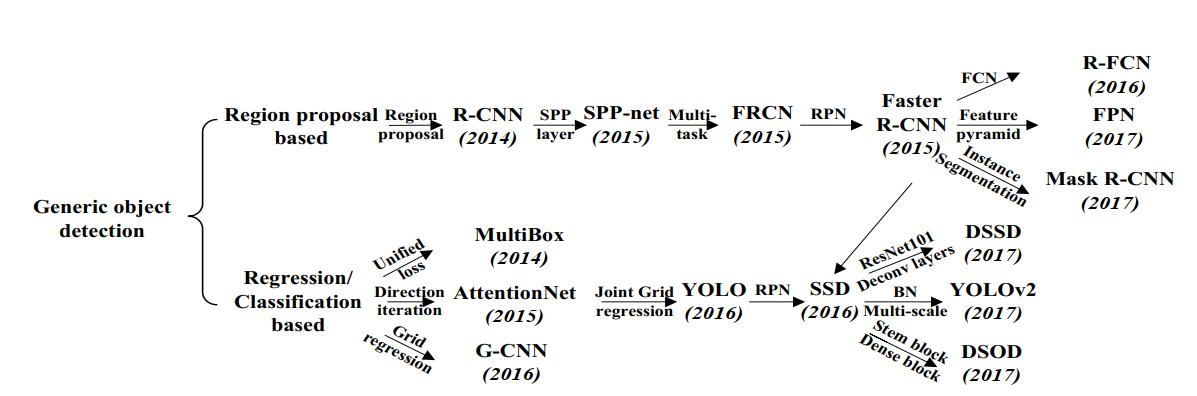
\includegraphics[width=14cm]{Images/recognition/Object_Detection.png}
\caption{Object detection}
\label{fig:object detection}
\end{figure}

There are two main groups in CNN-based detection: ''two stages detecion'' and ''one stage detection''. In the first group, firstly the image will be examined to generate proposals, and these proposals are delivered to another network for classification. In the second group, the object will be detected and classified directly within one network model.

\subsubsection{CNN-based Two Stages Detection (Regional Proposal based)}
Released in 2014 by Girshick et al.\cite{17,18}, R-CNN is the first attempt in building a Convolutional Neural Network for object detection. The idea of R-CNN is divided into three main stages:
\begin{itemize}
    \item Proposals are generated by selective search.
    \item Proposals are resized to fixed resolution. These proposals are then used in CNN model to extract the feature map.
    \item Feature map is classified using SVMs for multiple classes to provide the final bounding box.
\end{itemize}
Despite having certain advantages comparing with traditional methods and bringing CNN back to practical use, R-CNN has some fatal disadvantages. The training has multiple stages and feature maps are stored separately thus increase time and space complexity. Moreover, The number of overlapped proposals are really high (over 2000 proposals for an image). The CNN model also requires a fixed size image, so any input must be resized and in certain occasions the object may get cropped, creating unwanted distortion.
    
Later in the same year, He et al. introduced a novel CNN architecture named SPP-Net \cite{29} using Spatial Pyramid Matching (SPM) \cite{30,31}. The Convolutional Neuron Network is combined with a Spatial Pyramid Pooling (SPP) layer, make the network able to generate a fixed length feature representation without scaling the input image. The model removes the proposal overlapping and the need to resize image, however, it still require a multi-step training including feature extraction, network fine-tuning, SVM training and bounding box regressor. Additionally the convolution layers before the SPP cannot be modified with the algorithm shown in \cite{29}
    
In 2015, Girshick proposed Fast R-CNN \cite{32}, a model with ability to do multi-task on classification and bounding box regression within the same network. Similar to SPP-Net, the whole image is processed with convolution layers to produce feature maps. Then, a fixed-length feature vector is extracted from each region proposal with a region of interest (RoI) pooling layer. Each feature vector is then fed into a sequence of fully connected layers before branching into two output, one is then used for classifier and the other encodes the bounding box location. Regardless of region proposal generation, the training of all network layers can be processed in a single stage, saving the extra cost on storage. 
    
In the same year, Ren et al. introduced Faster R-CNN, a method to optimize Fast R-CNN further by altering the proposal generation using selective search by a similar network called the Region Proposal Network (RPN) \cite{33}. It is a fully-convolutional network which has the ability to predict object bounds and scores at each position as the same time. With the proposal of Faster R-CNN, region proposal based CNN architectures for object detection can be trained
in an end-to-end way. However, the alternate training algorithm is very time-consuming and RPN does not perform well when dealing with objects with extreme scales or shapes. As a result, multiple adjustments have been made. Some noticeable improvements are Region-based fully convolutional network (R-FCN) \cite{34}, Feature Pyramid Network (FPN) \cite{35}, and Mask R-CNN \cite{36}. We will look in the details of these methods in the next chapter.

\subsubsection{CNN-based One Stage Detection (Regression/Classification based)}
Region proposal based frameworks are composed of several correlated stages, including region proposal generation, feature extraction, classification and bounding box regression. Even in Faster R-CNN or its variant, training the parameters is still required between the Region Proposal Network and detection network. As a result, achieving real time detection with Two Stages Detection is a big challenge. One Stage Detection, on the other hand, deal with the image directly by mapping image pixel to bounding box coordinates and class probabilities. 

\begin{itemize}
    \item You Only Look Once (YOLO):
    YOLO \cite{37} was proposed by J.Redmon et al. in 2015 as the first entry to the One Stage Detection era. This network divides the image into regions and predicts bounding boxes and probabilities for each region simultaneously. The YOLO consists of 24 convolution layers and 2 FC layers, of which some convolution layers construct ensembles of inception modules with 1 × 1 reduction layers followed by 3 × 3 conv layers. Furthermore, YOLO produces fewer false positives on background, which makes the cooperation with Fast R-CNN become possible. An improved version, YOLO v2,v3 and v4 was later proposed in, which adopts several impressive strategies, such as BN, anchor boxes, dimension cluster and multi-scale training.\cite{38,39,40}.

    \item Single Shot MultiBox Detector (SSD):
    SSD \cite{41} was proposed by W. Liu et al. in 2016 as the second entry of the One Stage Detector. SSD introduces the multi-reference and multi resolution detection techniques which significantly improves the detection accuracy. The main difference between SSD and any other detectors is that SSD detects objects of many different scales on different layers of the network rather than detect at the final layer.
    
    \item RetinaNet:
    RetinaNet \cite{42} uses a Feature Pyramid Network(FPN) with a CNN-based Backbone. FPN involves adding top level feature maps with the feature maps below them before making predictions. It usually involves upscaling the top level map, dimensionality matching of the map below using a 1x1 Convolution and performing element wise addition of both. RetinaNet achieves comparable result to Two Stages Detection while keeping much higher speed. 
    
    \item Refinement Neural Network for Object Detection (RefineDet):
     RefineDet \cite{43} is based on a feed forward Convolutional Network that is similar to SSD, produces a fixed number of bounding boxes and the scores indicating the presence of different classes of objects in those boxes, followed by the non-maximum suppression to produce the final result. RefineDet is formed by two inter-connected modules:\\
     $\bullet \quad$ Anchor Refinement Module (ARM): Remove negative anchors and adjust the locations/sizes of anchors to provide initialization for the regressor.\\
     $\bullet \quad$ Object Detection Module (ORM): do regressing object locations and predict multi-class labels based on the refined anchors.\\
     There are three core components in RefineDet: Transfer Connection Block (TCB) converts the features fro ARM to ODM; Two-step Cascaded Regression does regressing the locations and sizes of objects; Negative Anchor Filtering will reject well-classified negative anchors and reduce the imbalance problem. Further information will be discussed in the next chapter.
\end{itemize}

\section{Diagram detection}
In general, diagram detection can be grouped into two smaller areas: Online Diagram Recognition and Offline Diagram Recognition. In online recognition, the model is usually a RNN to recognize each stroke and generate candidate matches.
Valois et al. \cite{44} proposed a method for recognizing electrical diagrams. Each set of ink strokes is detected as a match with corresponding confidence factor using probabilistic normalization functions. Its disadvantage is the simplicity of the system and their low accuracy, prevent it from being used in real situations. Feng et al. \cite{45} used a more modern technique in detecting electrical circuits. Symbol hypotheses generation and classification are generated using a Hidden Markov Model (HMM) and traced on 2D-DP. However, it has a drawback of complexity when the diagram and number of hypotheses is large, makes it impractical for real life cases. ChemInk \cite{46}, a system for detecting chemical formula sketches, categorizing strokes into elements and bonds between them. The final joint is performed using conditional random fields (CRF), which combines features from a three layers hierarchy: inkpoints, segments and candidate symbols. Qi et al \cite{47}. used a similar approach to recognize diagram structure with Bayesian CRF - ARD. These methods outperforms traditional technique, but the difficulty in joining the features using pairwise at the final recognition step make them harder for future adaptations. Coming to Flowchart recognition, after the release of the Online Handwritten Flowchart Dataset (OHFCD), multiple researches took place in resolving this dataset. Lemaitre et al \cite{48}. proposed DMOS (Description and MOdification of the Segmentation) for online flowchart recognition. Wang et al. \cite{49} used a max margin Markov Random Field to perform segmentation and recognition. In \cite{50} they extend their work by adding a grammatical description that combines the labeled isolated strokes while ensuring global consistence of the recognition. Bresler et al. proposed a pipeline model where they separate strokes and text by using a text/non-text classifier then detect symbol candidates using a max-sum model by a group of temporally and spatially close stroke. The author also propose an offline extension that uses a preprocessing model to reconstruct the strokes from flowchart \cite{51,52}.

While online flowchart recognition detects candidates based on stroke, offline flowchart recognition receives an image from the user and use it to generate the diagram. It might be possible to reconstruct online stroke from offline data \cite{53}, however, that preprocessing step might not be necessary because we can recognize the whole diagram structure independently with strokes. As online recognition seem to attract more researchers, there has not been many studies about offline detection. A. Bhattacharya et al. \cite{54} uses morphological and binary mapping to detect electrical circuit. Although it may work on a smaller scale, using binary mapping may not be able to detect curve or zig-zag lines. Julca-Aguilar and Hirata proposed a method using Faster R-CNN to detect candidates and evaluate its accuracy on OHFCD. The model is able to detect components in the diagram, including arrows, however, it is not able to detect the arrow head. 
\section{Handwriting character recognition techniques for English alphabets} 
Handwriting recognition is a study domain in fields of image processing and pattern recognition which is popular and complicated in the current day. It contributes immensely to the
sequence of a computerization technique and could enhance the interface among human and machine in so many purposes. This process primarily start with preprocessing procedure which is followed by line segmentation, normalization, feature extraction, recognition and transcriptions according to \cite{12}. The preprocessing includes the process that improves the structure of the image which is more suitable in segmentation. In the segmentation procedure, the raw image is segmented into single characters and after that, the procedure reconstruct each character in m x n pixels to the training network. Next is about feature extraction technique, which affects recognition percentage. There are numerous of feature extraction methods which are mentioned in the research of \cite{13}. Additionally, according to \cite{12}, the frequently used feature extraction techniques are Contour profiles, Deformable templates, Fourier descriptors, Gabor
features, Gradient feature, Graph description, Geometric moment invariants, Template matching, Unitary Image transforms, Projection Histograms, Zoning, Zernike Moments and Spline curve approximation.
\subsection{Preprocessing}
In preprocessing procedure, there are many actions needs to be executed, which are noise removing, binarization, edge detection, dilation and filling, processed image for feature extraction according to \cite{12}. In noise removing phase, the reason for this phase is that scanned documents can be contaminated with dust, dots, or lines, which are classified as noise that has a negative impact on the recognition results. Therefore, image is applied with smoothing and non linear operations to improve the image quality. In addition, for text line which is not horizontally align during scanning process, the skew correction can be applied on the document or line level. In the preprocessing procedure, skew correction is applied on the document level.
\subsection{Line segmentation}
In line segmentation, this phase separates the image whose structure in a sequence of alphabet characters into sub image which contains a single character by conveying a number to every alphabet utilizing a labeling procedure. This labelling provides knowledge about number of characters in the image. Every single character is restructured into 90*60 pixels for categorization and recognition stage.
\subsection{Normalization}
After line segmentation, normalization is performed to eliminate the differences that complicate the categorization and decrease the recognition percentage of the similar character or word across different writers. The most general basis of variability in handwritten alphabet images is incline and text volume according to \cite{12}. Slant correction techniques is applied to correct the inclination in the writing style. By applying a shear transformation, the writings slant is transformed into its upright position. A shear transformation is applied in many directions. For each direction, the transformed image data are added with pixel values of the same image that are vertically shifted by distance d and –d.
\subsection{Feature extraction}
In feature extraction step, there are two main approaches which are used holistic and analytic \cite{12}. In holistic recognition, each word is considered to a class and is recognized as whole word. On the other hand, the other approach is based on character segmentation-free recognition.
Based on \cite{12}, features used in holistic offline recognition systems are categorized into high,
middle, and low levels. The high level removes the features from the entire phrase image, the middle level removes features from the letters, and the low level removes features from the sub letters. There are various types of holistic features which are represents in \cite{12}.
In analytic recognition schemes, the image is representing as a chain of characteristics. This scheme uses a slicing window which is shifted from left to right. At each position n, a characteristic vector fn is calculated from just the pixel within the slicing window. Two major slicing window scheme characteristics are profile characteristics and window characteristics \cite{12}.
\subsection{Recognition}
The English alphabets might be scripted in various size, direction, width, arrangement and measurement \cite{12}. Thus, recognition of English alphabets is extremely difficult problem. There are some frequently used learning models in this recognition process such as HMM (Hidden Markov Model), NN (Neural Network) and so on.
\chapter{Background}
\label{chap:background}
	\textit{In this chapter, we introduce the foundation knowledge of the thesis, including the history and definition of Blockchain Technology, Cryptocurrency, 
	Hierarchical Deterministic Wallet (HD Wallet) and Cryptography}
\minitoc

\section{Blockchain Technology}

\subsection{History and Definition}

Blockchains are immutable digital ledger systems implemented in a distributed fashion (i.e., without a central repository) and usually without a central authority.
The definition of blockchain was introduced to the world by a person (or a group of people) under the name Satoshi Nakamoto on October 31, 2008. 
It was applied to enable the emergence of a "purely peer-to-peer (no financial institution or third party) electronic cash" named Bitcoin where transactions take place in a distributed system.
In fact, Satoshi did not invent blockchain, and Bitcoin blockchain is not the first chain that ever created. 
Back in 1991, cryptographers Stuart Haber and Scott Stornetta published a whitepaper "How to Time-Stamp a Digital Document" in the Journal of Cryptography. 
Their goal is to digital time-stamping of documents so that it is infeasible for a user either to back-date or to a forward-date digital document, even with the collusion of a time-stamping service. 
The technology is called a blockchain because the distributed electronic ledger stores items of data in time-stamped digital groups called blocks. Each block includes an alphanumeric code called a "hash" summing up its data. The hash of each completed block also appears in the next one in the chain, which means that to alter one block you would have to alter all the ones connected to it. These cryptographic dominos function together to protect against tampering or fraud.
Base on this theory, the longest-running blockchain, started in 1995, also by Haber and Stornetta, publishes the weekly summary hash value every week in the New York Times (\autoref{fig:first_blockchain}) and still running strong today. 

\begin{figure}[h!]
	\centering
	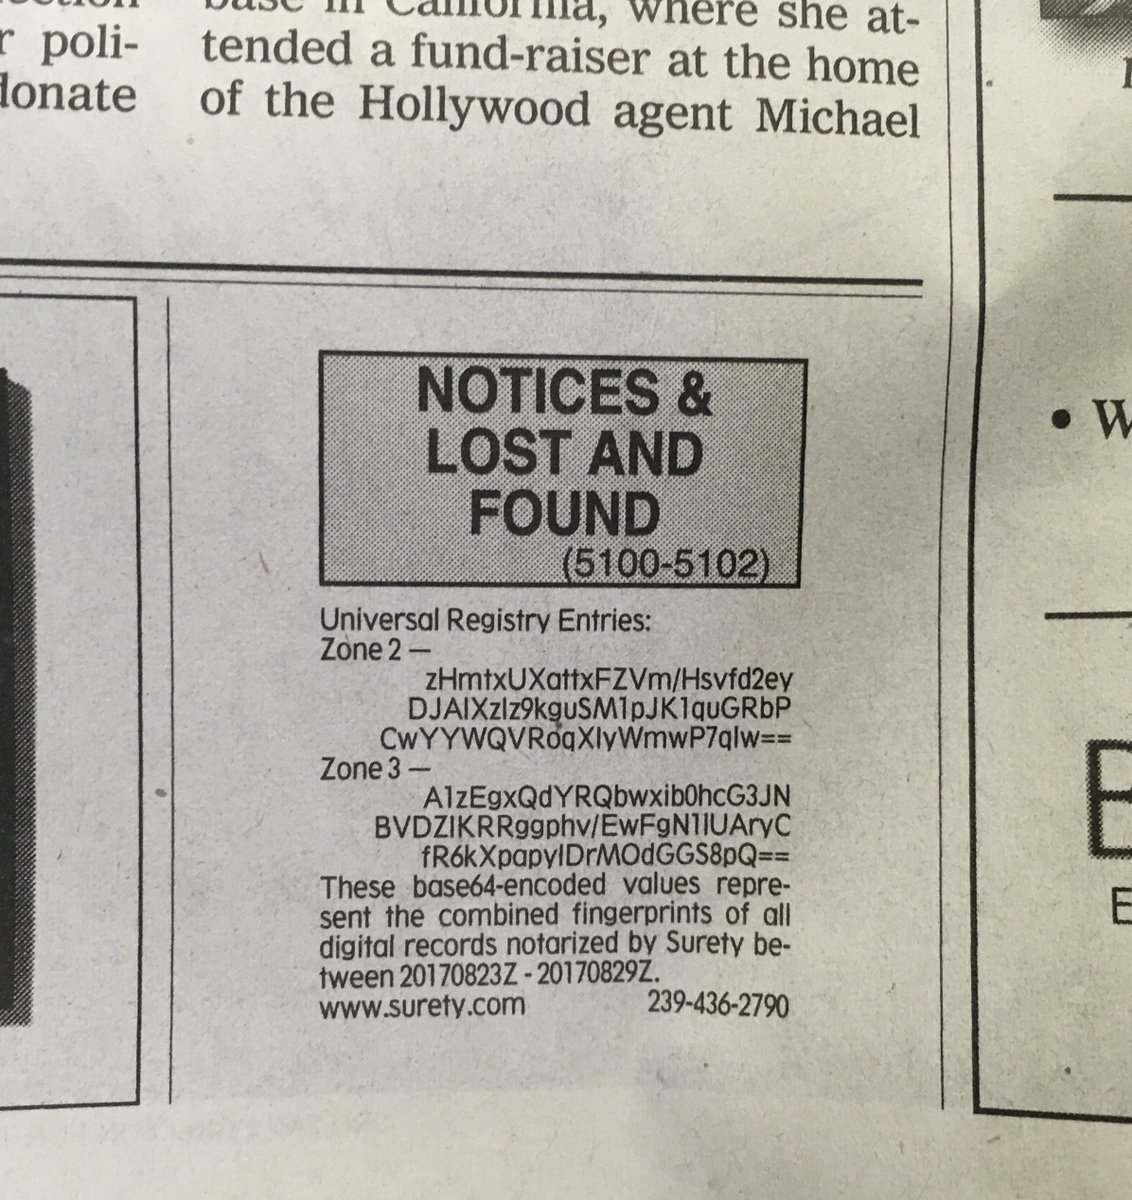
\includegraphics[width=.35\textwidth]{images/Widely_Witnessed_Values.jpg}
	\caption[Widely-Witnessed Values of Surety, a weekly summary (hash) of documents]{Weekly summary hash value in The New York Times}
	\label{fig:first_blockchain}
\end{figure}

% The math behind blockchain and its complex system architecture make it challenging to understand. 
But the word "blockchain" or "block" and "chain" wasn't use back then. 
Only it become known in Satoshi Nakamoto's Bitcoin paper in the term of "chain" of "blocks".
Later people combined the one-word "blockchain" in mainstream media publications such as Fortune, Forbes, and the Huffington Post as the technology gained greater interest and use. 
The comunity use that word for Nakamoto's invention.
Bound to emergence of Bitcoin and cryptocurrency, a concise description of blockchain technology is provided by NIST:

\begin{quote} 
	Blockchains are distributed digital ledgers of cryptographically signed transactions that are grouped into blocks. Each block is cryptographically linked to the previous one (making it tamper evident) after validation and undergoing a consensus decision. As new blocks are added, older blocks become more difficult to modify (creating tamper resistance). New blocks are replicated across copies of the ledger within the network, and any conflicts are resolved automatically using established rules.
\end{quote}

Blockchain technology comes handy in a wide range of areas - both ​financial and non-financial​. 
Non-Financial application opportunities are endless. 
We can envision putting proof of the existence of all legal documents, health records, and loyalty payments in the music industry, notary, private securities and marriage licenses in the blockchain. 
By storing the fingerprint of the digital asset instead of storing the digital asset itself, the anonymity or privacy objective can be achieved.
For the sake of our thesis, we will mainly focus on the original and surely the most popular application of blockchains - Cryptocurrency.

Cryptocurrencies are digital currencies that use blockchain technology to\autoref{fig:first_blockchain}) and still running strong today. 
record and secure every transaction. 
A cryptocurrency can be used as a digital form of cash that can be used to buy goods and services. 
It can be bought using one of several digital wallets or trading platforms, then digitally transferred upon purchase of an item, with the blockchain recording the transaction and the new owner. 
The appeal of cryptocurrencies is that everything is recorded in a public ledger and secured using cryptography, making an irrefutable, timestamped, and secure record of every payment.
The ledger displays user account balances and inter-user payments in a “currency” defined by the ledger itself and not necessarily in one of the traditional currencies. 
Nevertheless, cryptocurrency may be traded on the stock exchange and exchanged for traditional money, which makes it hard to distinguish between traditional currency and cryptocurrency and as official vs. non-official currency. 
The most widely recognized cryptocurrency system is Bitcoin.

We believe the "magic" that brings the above concept of digital currencies to reality, besides blockchain technology, is Nakamoto's proof-of-work consensus model.

\subsection{Blockchain Categorization and Generations}

Blockchain systems can be:
\begin{itemize}
	\item \emph{Permissioned blockchain}, where users publishing blocks must be authorized by some authority (be it centralized or decentralized). 
	Users of blockchain have to trust that entity or user who published blocks. 
	Permissioned blockchain networks may thus allow anyone to read the blockchain or they may restrict read access to authorized individuals. This maybe used by organizations that need more control over their blockchain.
	Some permissioned blockchain networks support the ability to selectively reveal transaction information based on a blockchain network users identity or credentials. 
	Some of famous permissioned blockchain applications are Ripple, which enables interbank transactions, or Sovrin, which is managed by financial institutions and is seeking to build a global decentralized identity system.
	
	\item \emph{Permissionless blockchain}, where service providers are not fixed and, in principle, anyone can start operating the service. For example, Bitcoin and the early versions of Ethereum.
	
\end{itemize}

% The blockchain is usually stored and managed in the form of a distributed ledger,
% with multiple parties keeping a copy of the ledger, which then implies the use of a
% handshake protocol between the components. However, also centralized blockchain
% system exist. The original and surely the most popular application of blockchains is
% cryptocurrency, where the ledger displays user account balances and inter-user payments
% in a “currency” defined by the ledger itself and not necessarily in one of the traditional
% currencies. Nevertheless, cryptocurrency may be traded on the stock exchange and
% exchanged for traditional money, which makes it hard to distinguish between traditional
% currency and cryptocurrency and as official vs. non-official currency. The most widely
% recognised cryptocurrency system is Bitcoin, which establishes and uses Bitcoins and
% Satoshis as currency.

% Most permissionless blockchain systems include an independent cryptocurrency. 
% The reason for that is that in the absence of an inter-operator contract, there are usually no other incentives to guarantee voluntary management of the Blockchain

Based on the intended audience, three generations of blockchains can be distinguished (Zhao et al., 2016):
\begin{itemize}

\item Blockchain 1.0 which includes applications enabling digital cryptocurrency transactions
\item Blockchain 2.0 which includes smart contracts and a set of applications extending beyond cryptocurrency transactions
\item Blockchain 3.0 which includes applications in areas beyond the previous two versions, such as government, health, science and IoT.

\end{itemize}

We are now developing blockchain 2.0 but our thesis just focus on cryptocurrency aspect.


\subsection{Bitcoin blockchain}
Bitcoin is the first application of blockchain and the most famous digital currency ever.
As mentioned above, Bitcoin was invented with the publication of a document entitled "Bitcoin: A peer-to-peer electronic cash system" in 2008 by Satoshi Nakamoto, mentioned as a purely P2P version of electronic cash would allow online payments to be sent directly from one party to another without going through a financial institution. 
The currency began to use in 2009 when its implementation was released as open-source software. 
The Bitcoin blockchain is considered to be a world-changing technology because in the first time in human history its solved the biggest problem of distributed system: The Byzantine General's Problem. 
We will talk about this in the Bitcoin game of theory and incentives section.

Bitcoin application is one of the permissionless blockchain.
It utilize well-known computer science mechanisms (linked lists, distributed networking) as well as cryptographic primitives (hashing, digital signatures, public/private keys) mixed with financial concepts (ledgers, games of theory) in high level. 
Base on the problems Bitcoin has solved, we examine by dividing it into 3 components:

\begin{itemize}
\item Secure and Prevent tempering the data

\begin{quote} 
	\emph{Hashes} - 
	Cryptographic hash functions (CHF) are used for hashing the content of a block, validating the integrity of data, reduce the size of the message or keys, generating a Bitcoin address. We will show detail at Section~\ref{sec:crypto_hash}.
	Hashing is a method of calculating a relatively unique fixed-size output (called a message digest, or just digest) for an input of nearly any size (e.g., a file, some text, or an image).
	Even one single bit change of input will result in a completely different output digest. 
	In Bitcoin and most blockchain technologies, SHA-256 (Secure Hash Algorithm with output size of 256 bits) appear the most. Many computer support hardware level for this algorithm.
	NIST specified this algorithm for SHA-256 in Federal Information Processing Standard (FIPS) 180-4 as it passed every properties of a cryptographic hashing.
	\autoref{fig:example_of_sha-256} is an example of SHA-256.

		\begin{figure}[h!]
			\centering
			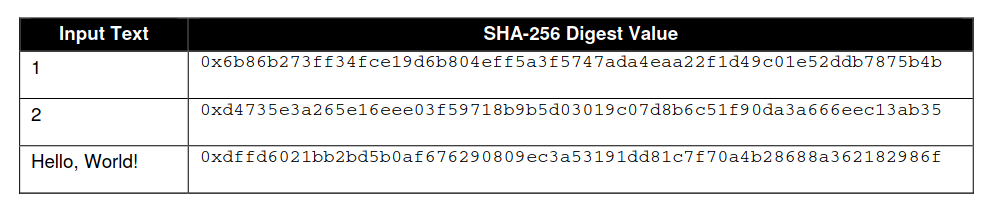
\includegraphics[width=1\textwidth]{images/example_of_sha-256.png}
			\caption[Example input and output of SHA-256 Digest Value]{Example I/O of SHA-256 Digest Value}
			\label{fig:example_of_sha-256}
		\end{figure}

	\bigbreak
	
	\emph{Public/Private Key} -	
	Asymmetric-key cryptography (or public-key cryptography) uses a pair of keys: a public key and a private key that are mathematically related. It could be infeasible to generate one key from the other.
	The private key is kept secret while the public key can be to everyone, both keys are hold inside user's Wallet, which we present in Section~\ref{sec:hd_wallet}.
	One can encrypt with a private key and then decrypt with the public key. 
	Alternately, one can encrypt with a public key and then decrypt with a private key.
	Bitcoin uses asymmetric-key cryptography to digitally sign transactions, verify signatures or in some cases, exchange the key.
	Asymmetric-key cryptography is discussed in Section~\ref{sec:asymmetric_cryptography}.
	Figure~\ref{fig:asymmetric_cryptography} briefly show message exchange usage of the asymmetric protocol.
	
	\begin{figure}[h!]
		\centering
		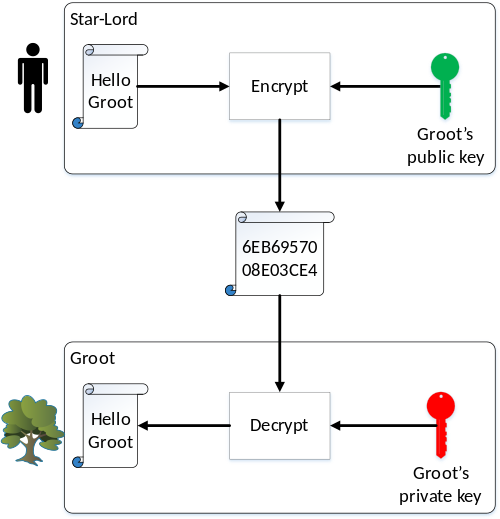
\includegraphics[width=0.4\textwidth]{images/asymmetric_cryptography.png}
		\caption[An example of concept of Asymmetric-key cryptography]{Sending private message using Asymmetric-key cryptography}
		\label{fig:asymmetric_cryptography}
	\end{figure}
	\bigbreak

	\emph{Transactions} - Transactions represent transfers of the cryptocurrencies between wallets in the system. 
	A transaction contains input and output. The inputs are usually a list of the digital assets to be transferred.
	Outputs are	the accounts that will be the recipients of the digital assets along with how much digital asset they will receive.   
	All values of in and out cannot be tampered.

	\begin{figure}[h!]
		\centering
		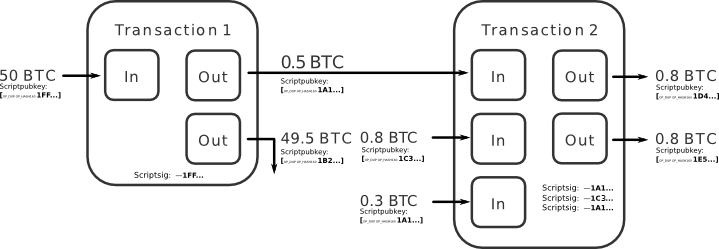
\includegraphics[width=0.7\textwidth]{images/transaction.png}
		\caption[An example of bitcoin transaction]{An example of bitcoin transaction}
		\label{fig:transaction}
	\end{figure}
	\bigbreak

	All transactions are broadcast to the network and usually begin to be confirmed within 10-20 minutes, through a process called \emph{mining}.
	Transactions are typically digitally signed by the sender’s associated private key and can be verified using the associated public key.

	\bigbreak

	\emph{Ledgers} - 
	A ledger is a collection of cryptographic transactions. 
	Bitcoin ledgers are distributed, the blockchain holds all accepted transactions within its ledgers. Every user can maintain their own copy of the ledger.
	Whenever new full nodes join the blockchain network, they reach out to discover other full nodes and request a full copy of the blockchain network’s ledger, making loss or destruction of the ledger difficult.
	\bigbreak
	
	The network utilizes cryptographic mechanisms such as digital signatures and cryptographic hash functions to provide tamper-evident and tamper-resistant ledgers.
	Due to the public distributed network, the Bitcoin blockchain is harder to attack. There is nothing to steal because everything is distributed. If one individual node got taken down, the network will still be running. 
	If targeting the blockchain itself, the attackers will face resistance from the honest nodes present in the system. 
	\bigbreak

	\emph{Blocks} -	
	Transactions, after sent to the network (by wallets, web applications, etc.), will be, if accepted, added to a block that is published by a chosen node. 
	Bitcoin blocks include block header and block data.
	Figure~\ref{fig:block_component} show basic component of a block.
	Block header contains version, previous block header’s hash value (prevBlockHash), a hash representation of the block data (usual Merkle tree* hash), a timestamp, size of the block (bits), a \emph{nonce}.
	The \emph{nonce} value is manipulated by the publishing node to solve the hash puzzle (see Section~\ref{subsec:game_theory})
	Block data contains a list of transactions and ledger events. Some include other data.
	\pagebreak

	\begin{figure}[h!]
		\centering
		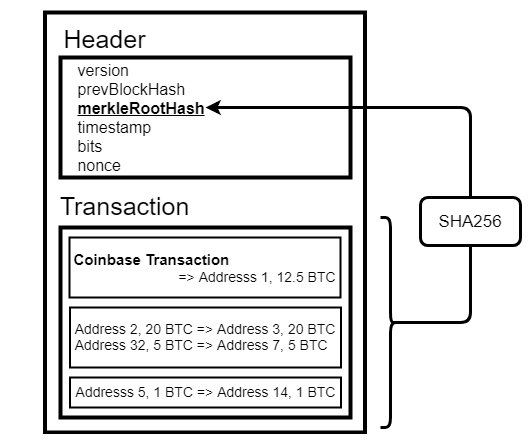
\includegraphics[width=0.6\textwidth]{images/block_component.jpg}
		\caption[Components of Bitcoin block]{Components of Bitcoin block}
		\label{fig:block_component}
	\end{figure}

	\emph{Chain of Blocks} - 
	Blocks are chained together through each block containing the hash digest of the previous block’s header, thus forming the blockchain.
	If one of the previous blocks were changed, it would result in a different hash.
	This makes it possible to easily detect and reject altered blocks

	\begin{figure}[h!]
		\centering
		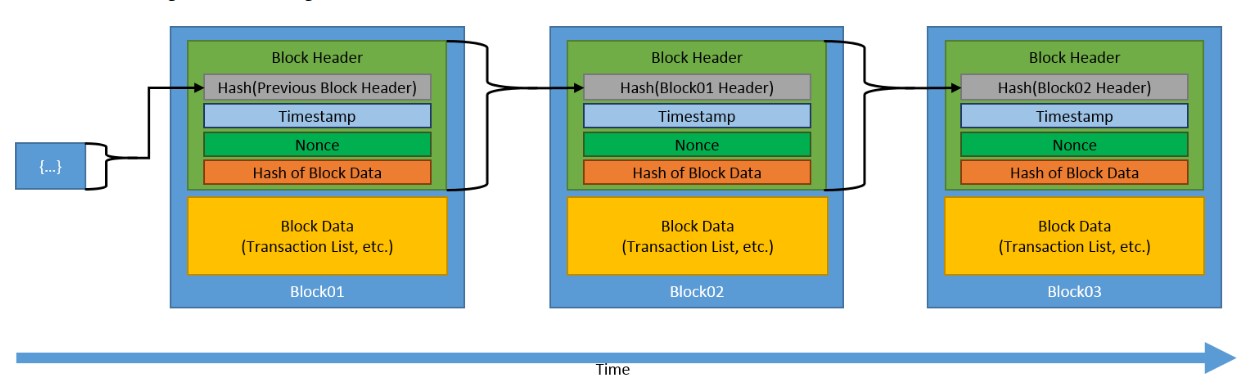
\includegraphics[width=1\textwidth]{images/chain_of_block.png}
		\caption[Components of Bitcoin block]{Components of Bitcoin block}
		\label{fig:chain_of_block}
	\end{figure}


\end{quote}

\item Game of theory and Incentives
\label{subsec:game_theory}

\begin{quote} 
	\emph{Hashes} - 
	Cryptographic hash functions (CHF) are used for hashing the content of a block, validating the integrity of data, reduce the size of the message or keys, generating a Bitcoin address. We will show detail at Section~\ref{sec:crypto_hash}.
	Hashing is a method of calculating a relatively unique fixed-size output (called a message digest, or just digest) for an input of nearly any size (e.g., a file, some text, or an image).
	Even one single bit change of input will result in a completely different output digest. 


\end{quote}
\item Communication Network

\begin{quote} 
	\emph{Hashes} - 
	Cryptographic hash functions (CHF) are used for hashing the content of a block, validating the integrity of data, reduce the size of the message or keys, generating a Bitcoin address. We will show detail at Section~\ref{sec:crypto_hash}.
	Hashing is a method of calculating a relatively unique fixed-size output (called a message digest, or just digest) for an input of nearly any size (e.g., a file, some text, or an image).
	Even one single bit change of input will result in a completely different output digest. 

\end{quote}

\end{itemize}



\section{HDWallet}
\label{sec:hd_wallet}

\subsection{Blockchain wallet}
A blockchain wallet, sometimes referred as a cryptocurrency wallet, is a program that allows you to “store”, send and receive digital currencies. Since cryptocurrency doesn’t exist in any physical form, your wallet doesn’t hold any of your coins actually. Instead, it tracks the transactions you made, which is stored in blockchain, and then infers your balance. Thereby, blockchain is an essential component of a blockchain wallet.

Instead of holding physical coins, a wallet has a public key and a private key. Public key is a long sequence of letters and numbers that forms the wallet address. With this, people can send money to the wallet. It's similar to a bank account number in that it can only be used to send money to an account. Private key is used to access the funds stored in the wallet. With this, people can control the funds tied to that wallet's address. It's a lot like your PIN number in that you should keep it 100\% secret and secure. However, it's worth noting that not all wallets give you sole ownership of your private key, which essentially means that you don't have full control over your coins. As well as storing your public and private keys, crypto wallets interface with the blockchains of various currencies so that you can check your balance and send and receive funds.

\subsection{Category}

Now that you know what is, let’s take a closer look at the five different types of wallets available, each with its own advantages and disadvantages in terms of security, ease of use, convenience and a range of other factors. The most common type of wallet out there, desktop wallets are downloaded and installed on your computer. Easy to set up and maintain, most are available for Windows, Linux and Mac, although some may be limited to a particular operating system. Many cryptocurrencies offer a desktop wallet specifically designed for their coin.

Desktop wallets provide a relatively high level of security since they’re only accessible from the machine on which they’re installed. The biggest disadvantage is that they also rely on you to keep your computer secure and free of malware, so antivirus and anti-malware software, a strong firewall and a common-sense approach to security are required to keep your coins safe. Most desktop wallets will provide you with a long string of words upon installation. These words are known as your recovery seed or sentence and map with your private key, so it’s important to store them somewhere safe in case your computer dies or you need to format the operating system and re-install your desktop wallet. Some popular desktop wallets: Electrum, Exodus, Copay.

Mobile wallets are fairly similar to desktop wallets, with the obvious difference being that they run as an app on your smartphone. Mobile wallets feature many of the same advantages and disadvantages as desktop wallets, with your private key stored on your device.
Smartphone wallets are often easier to use compared to their desktop counterparts and include the ability to scan other wallet addresses for faster transactions. They also make it simpler to access your coins on the go and use cryptocurrency as part of everyday life. You will need to be extra careful about losing your smartphone, though, because there’s a risk that anyone who has access to your device might also have access to your funds. Choosing an app that allows you to back up your wallet with a 12- or 24-word passphrase is a good idea. Popular mobile wallets: Jaxx, Coinomi, Edge.

Online wallets (most often provided by exchanges but sometimes offered by third parties) are connected to the Internet and are generally the easiest to set up and use. Most only require an email address and a password to create an account, and web wallets are usually designed to provide a simple and straightforward user experience. The biggest advantages to online wallets are that they can’t be lost and that they’re accessible from any computer with an Internet connection. However, being online is unfortunately also their biggest disadvantage. Because some platforms maintain the wallets of thousands of users, they can become hot targets for hackers. It’s also important to check whether the wallet you choose lets you retain complete control of your private keys or whether they’re owned by the wallet provider. Popular web wallets: blockchain.info, MyEtherWallet, Coinbase.

Hardware wallets add another layer of security by keeping your private key on a USB stick or specially designed piece of hardware. They allow the user to plug the USB stick into any computer, log in, transact and unplug – so while transactions are carried out online, your private key is stored offline and protected against the risk of hacking. As a result, hardware wallets are widely considered to offer the most secure storage option. The biggest disadvantage of hardware wallets is that they’ll cost you. Prices vary depending on the model you choose, but they generally cost upwards of \$150. You also need to keep the device safe, but if you do lose your hardware wallet, the device itself is PIN-protected and there are usually other protective measures in place to help you recover your funds. Popular hardware wallets: Ledger Nano X, Ledger Nano S, TREZOR, KeepKey.

Paper wallets take the concept of entirely offline keys used for hardware wallets to the next logical step: simply print out your public and private keys and use that piece of paper as your wallet. As secure as they are, paper wallets are also complex and quite confusing for beginners. They’re typically only used by advanced users who want a high level of security. To transfer money to a paper wallet, you use a software wallet (any of the above mentioned) to send money to the public key printed on the sheet of paper. Most often, this is printed as a QR code for easy scanning. To transfer money from the paper wallet to someone else, you would first need to transfer money to a software wallet (by manually entering the private key into the software), and then transfer money from the software wallet to the recipient as usual. Popular paper wallets: Bitaddress.org, WalletGenerator.net.

As you’re researching and comparing a range of wallets, you’ll probably come across the terms “hot wallet” and “cold wallet”, or perhaps the concept of “cold storage”. So, what does temperature have to do with crypto storage?
A wallet is hot when it's connected to the Internet. Nothing on the Internet is 100\% secure, so funds kept in a hot wallet are always at a slight risk of theft or loss from software bugs or hackers. A wallet is cold when it's safely offline and can't be deliberately or accidentally compromised over the Internet.

\subsection{HDWallet}


\section{Cryptography}

\subsection{Cryptographic hash}
\label{sec:crypto_hash}

\subsection{Asymmetric-key cryptography}
\label{sec:asymmetric_cryptography}

\subsubsection{Diffie-Hellman algorithm}

\subsubsection{RSA Cryptography}

\subsubsection{ECC - Elliptic Curve Cryptography}

\subsection{Twisted-Edward curve and Ed25519}

\subsection{Child key derivation function}

\chapter{Proposed system} \label{chap:ProposedSystem}

\section{Project scope and restrictions}
\begin{itemize}
    \item The topic focuses on building mobile apps on Android platform using Flutter and the main programming language is Dart and doesn't support other mobile platforms like iOS, Windows Phone.
    \item User can only convert hand drawn diagram to digital version if internet connection is available.
    \item The web server can serve 100 clients at the same time.
    \item The system only supports converting and editing of small charts (in an A4 page, medium size text) and does not support importing files from other platforms.
    \item The system only create and editing flowchart.
    \item The system only supports storing chart files in .json format and exporting to images (png, jpg), text (pdf) and .drawio files.
    \item The flowchart contains maximum 20 symbols not including arrows
    \item The system do not allow to take picture with the wrong direction.
    \item The flowchart must not have three or more arrows intersect at one point. It also must not have two arrows having the same edge.
    \item The flowchart must be drawn with ball pen on a fresh white paper.
    \item Arrow in flowchart must have an arrowhead. 
    \item There must not be isolated text/symbol. Furthermore, strikethrough text is restricted.
\end{itemize}

\section{Application features}

The application runs on mobile devices so that users can easily convert a graph on the fly as long as they are connected to the internet. It also requires storage access and camera access permission in order to use the scanning function and temporarily saving it in the phone.

\subsection{Sign up and Login}
When users open the app for the first time, they will be offered to create an account to continue. To simplify the sign-up process, it only requires the user's email and password. Other information can be updated later on. In addition, users can also use their Google account to sign in without creating their own account for this app. In case users had already forgotten the password, they can retrieve it by providing their account email and the system will send an email to verify and include further information for changing the password.

\subsection{Create diagram}
After successfully login in, users can create a new diagram using one of these methods:
\begin{itemize}
    \item Directly Scanning: The application activates the device's camera so user can point at the drawing and take a picture of it.
    \item Import from image: User selects an image from device's gallery.
    \item Create blank: User can create a blank diagram and add elements then.
\end{itemize}

\subsubsection{Convert to digital}
If user chooses the first two options then after taking/choosing the picture he/she can re-take or re-adjust the picture (rotate, flip, or crop) before finishing this step. After that, the result will be displayed and provide some extra options: save, modify, and delete. Save option will require inputting the diagram name and choose the saving location. The diagram can be saved online on the web server or offline on the phone. Each user can only save a limited number of diagrams online, if a user is running out of saving slot then the only option is to store them locally. The main difference between saving online and offline is only the diagrams on the web server can be shared and have a detailed change history. Modify option is used if user is not satisfied with the result of the auto-detection algorithm and want to change it. This option will send them to the modify page where they can edit it before saving. Note that if user leaves this page without saving it, the diagram will be lost. Delete option shows a confirmation message and offers a retry.

\subsubsection{Create from blank}
If ``Create blank'' is chosen then a name for new diagram is required, then user will be sent to modify page where already has a default diagram created.

\subsection{Adjust diagram}
All the created diagrams will be displayed on the main screen of the app, user can select one of them to modify, delete, rename, view history change, export, and share. Only diagrams that are stored online have the share option and view history change option.

On the modify page, user can change elements' position, create new ones, or delete them. All elements supported will be listed later. All the attribute that user can change within an element is size, title, color, and type of element. All of the changes will be stored so that the user is able to undo or redo the action. Auto-saving is not supported, user needs to save manually. If user exits the app without saving, all of the progress will be lost.
"Change history" function requires to store a version of the old diagram every time a new one is saved into the web server. If the diagram is shared within a group, all of the information about the user who makes changes is also stored.

\subsection{Share and set permission}
Users can also share the diagram with others. However, only the owner can share their product. All of the shared diagrams will be in another tab on the home screen. To share a diagram, user needs to input the receiver's email and set their permission to "Read-only" or "Can edit". The Owner can also revoke the share permission by deleting the other user from the share list.

\section{Requirements}
\subsection{Functional requirement}
\begin{itemize}
    \item {System is able to detect the flow-chart diagram from a hand-drawing draft.}
    \begin{itemize}
        \item {System is able to detect the node type and its title.}
        \item {System is able to detect the relationship between the diagram’s symbols and check for incorrect relationship.}
        \item {System is able to detect the relationship between the diagram’s symbols and check for incorrect relationship.}
        \item {English is the main supported language.}
    \end{itemize}
    \item {System is able to re-create the diagram into digital version to display in the mobile application, and allow user to modify.}
    \item {The input can be directly taken from the camera of the device or uploaded from the storage.}
    \item {(Optional) System has the ability to convert the diagram to some popular diagram file format so that user can import it from tools like drawio, lucidchart, …}
\end{itemize}

\subsection{Nonfunctional requirement}
\begin{itemize}
    \item {System is written with Dart (with framework Flutter), C++.}
    \item {System is able to detect diagram within 8 seconds.}
\end{itemize}

\subsection{Hardware requirement}
\begin{itemize}
    \item {Mobile application require device must be installed with android OS version 7.0 or above }
    \item {Recommend requirement for web server:}
\end{itemize}
\chapter{System design} \label{chap:Systemdesign}

\section{System Architecture}
\begin{figure}[!b]
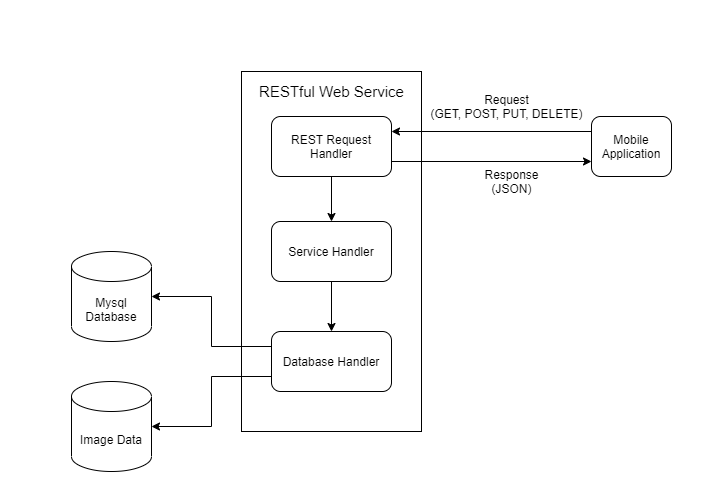
\includegraphics[width=14cm]{Images/App/System_Design.png}
\caption{System Architecture Design}
\end{figure}

At first, this application has two system options: One that requires no additional server to run, all of the service is installed locally on the user's devices. Since our core service, the diagram detection algorithm is written with C++ then it can run on any system. Then we intended to build an application system that can handle the whole process of pre-processing image and create the result without the internet connection. However, as our target is to support all the device that runs android 7.0 and above (that means all smartphones manufactured from 2016 to present and some of them can be older), it could lead to a performance problem because many of them were outdated 2 or 3 years. Another issue is sharing between users will have to be dependent on a third-party service. Which is not convenient and may lower the user experience.

The second one is to build a REpresentational State Transfer Application Programming Interface (REST API) service, run on a node.js server, which will handle all the requests sent by users and store all the data on a system database so that users can now store all of their data online without worry about their phone internal storage. the web server can be divided into three main components: Request handler, Service handler and Database handler. All of the detection and management will be mainly process in the second component, then all of the data will be transfer to a My SQL database, including user data and diagram file. However, all of the uploaded images that sent to the server to process will be then stored in the image storage separated from main database for additional data to improve detection algorithm in the future. The downside of this approach is now in order to use the app, the application has to be stably connected to the internet to make any changes to their data (create, edit, remove,...). Another challenge for us is to optimize the server so it can process a lot of access at the same time.



\section{Framework}
\subsection{Flutter}
Flutter is a user interface toolkit developed by Google for building beautiful, natively compiled applications for mobile, web, and desktop from a single code base \cite{57}. Dart is the main programming language used in Flutter.

One of the most beloved of Flutter that finally made it the framework we use in this thesis is it can create great and modernized user interfaces that really suit our design code for this project: simplistic but easy to use. Although the result can be used to build both android and iOS (potentially web) applications, the target of this project is to focus on one platform at first and continue to grow in the future. Despite being a recently released framework built for mobile development, Flutter provides a lot of features that speed up the development process as well as a growing community to share and learn.

However, there is also a downside of it, since it was born to build an application that can run on many different platforms, the performance loss is inevitable compared to natively built applications. Even though Flutter has been optimized and guarantee 60 frames per second but it still heavily depends on developers to make good use of available performance resources. Another one is the application file built by Flutter tends to have a bigger file size and also consume a lot more storage to install. A normal solution for this is to reduce image resolution and use less graphic and animations in the app, but Flutter still shows a poorer result than the native app.

\subsection{Nodejs}
Nowadays, Node.js is one of the most popular JavaScript Run time Environment as it is an open-source, cross-platform, and powerful tool that is used for many server-side projects \cite{59}. One of the biggest advantages is using JavaScript, which supports asynchronous programming. In the Node.js server, all requests will be handle by a single process without creating any thread. When a process requires queries in the database, the system allows pausing it until the queries are finished, in the meantime, other jobs can be handled without wasting a whole thread. As the number of clients increases over time, this can be a great feature to scale up the system.

\section{Database Design}

For each user, besides user name, email and password are essential information, an account must also have an account type to indicate whether it is a system account or from another platform account (such as Google). If so, it required another field to store the account ID key. If the account is created in the application then the password needs to be hashed and salted, which required 2 fields for salt string and encoded password. In order to perform any action with the server from the client-side, it requires a key for authentication each time the device calls an API, which will be changed each time a user logins. This key will be expired after half an hour of inactivity. Each time an API is called, the expired time will be refreshed. The expired time is stored with the user account for comparison each time this key is used. With this design, the system cannot keep track of the number of times a user logged in or how many times the API was called with a specific user key. However, all of the activities on the server will be recorded in other tables (creating and uploading diagram, send review), it will be unnecessary to create a table for login records.

Each diagram has to belong to a user, diagrams can be shared between users with different permission like ''Owner'', ''Edit-Only'', and ''Read-only''.

There can be two types of diagrams,  the ''converted'' diagram and the ''created from blank'' one. For the first type, it requires a field to store the image path in the image storage.

As each diagram may have many versions, each time the user uploads a new one, it will be stored with a new ID and also have an upload type to distinguish between new upload and revert (as the user is able to view the change history, they may also revert back to an older version), then it will need an additional field to store the reverted version in order not to store many same version of the same diagram file.

\begin{figure}[!b]
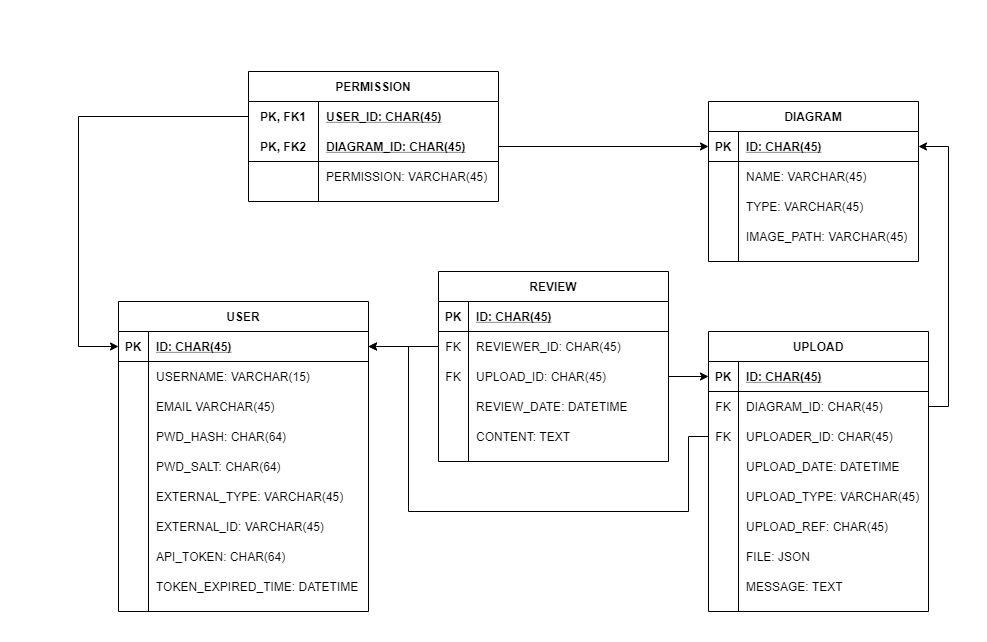
\includegraphics[width=16cm]{Images/App/DB.png}
\caption{Database Design}
\end{figure}

\section{Diagram File Design}
After having consulted some types of diagrams, we decided to go with .json file since it is widely used and supported by many platforms. It is also able to be stored directly in the My SQL database using JSON data type. Although the size still depends on the server configuration, this is one of the most convenient file types to transfer between the web server and the client devices. The file will have 4 main components: ID, name, an array of symbols, and an array of arrows.

Figure \ref{fig:jsonfile} shows the json file design used for construct the diagram used in the application.

\begin{figure}[!b]
\centering
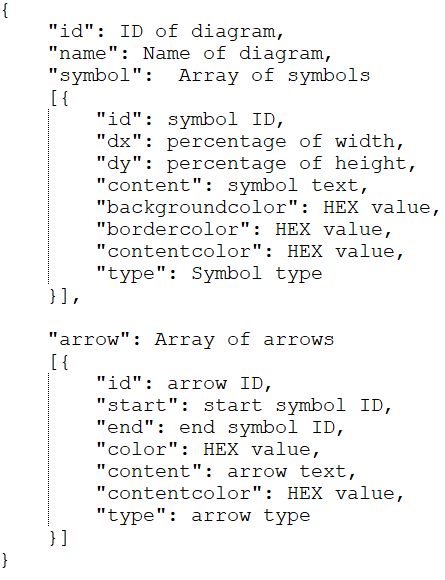
\includegraphics[width=12cm]{Images/App/jsonFile.png}
\caption{JSON file design}
\label{fig:jsonfile}
\end{figure}



\section{Use case Design}
\subsection{Use case diagram}
Figure \ref{fig:usecase} shows the system use case design for the application.

\begin{figure}[!t]
\centering
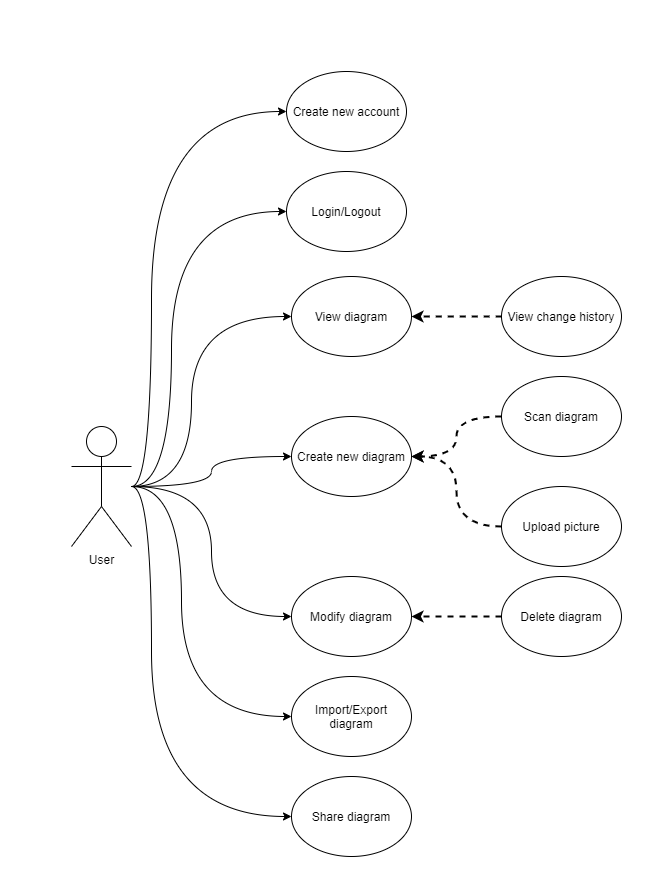
\includegraphics[width=14cm]{Images/App/Usecase.png}
\caption{Use case Design}
\label{fig:usecase}
\end{figure}

\subsection{Use case detail}
\begin{table}[b]
\begin{tabular}{| m{8cm} | m{6cm} |}
\hline
Use case name & Table reference\\ \hline
Login. & Table \ref{Tab:UC-1}\\ \hline
Sign up. & Table \ref{Tab:UC-2}\\ \hline
Create new diagram. & Table \ref{Tab:UC-3}\\ \hline
Scan diagram with camera. & Table \ref{Tab:UC-3.1}\\ \hline
Scan from image. & Table \ref{Tab:UC-3.2}\\ \hline
Import file. & Table \ref{Tab:UC-4}\\ \hline
Export file. & Table \ref{Tab:UC-5}\\ \hline
Modify diagram. & Table \ref{Tab:UC-6}\\ \hline
Delete diagram. & Table \ref{Tab:UC-7}\\ \hline
% Share. & Table \ref{Tab:UC-8}\\ \hline
% Set permission. & Table \ref{Tab:UC-9}\\ \hline
% View change history. & Table \ref{Tab:UC-10}\\ \hline
% Revert. & Table \ref{Tab:UC-11}\\ \hline
Logout. & Table \ref{Tab:UC-12}\\ \hline
\end{tabular}
\captionof{table}{\label{Tab:UCList}Use case List}
\end{table}

\begin{table}[]
\begin{tabular}{| m{4cm} | m{11cm} |}
\hline
Use case ID:       & UC-1 \\ \hline
Use Case Name:     & Login. \\ \hline
Triggering Event:  & The user open the app and in login screen. \\ \hline
Brief Description: & System verify user's inputted username and password and go to home screen. \\ \hline
Actors:            & The user \\ \hline
Preconditions:     & \begin{itemize}
    \item Application has internet connection.
    \item The user has a system account.
    \item The user has not logged in with Google account.
\end{itemize} \\ \hline
Post-conditions:   & \begin{itemize}
    \item The user is logged in to the system.
    \item The user is able to perform action that requires the web server.
\end{itemize} \\ \hline
Normal flows:      & \begin{enumerate}
    \item The user opens the app.
    \item System show login form including username and password.
    \item The user fill in the form and login.
    \item System authenticates user.
    \item The user is logged in and has access to the system.
\end{enumerate} \\ \hline
Alternative flows: & \begin{itemize}
    \item {2a The user has already logged in with Google account}
    \begin{itemize}
        \item 2a1 System automatically authenticates user in with Google account.
        \item 2a3 Use case continue with step 5.
    \end{itemize}
    \item {3a The user chooses to log in with Google account}
    \begin{itemize}
        \item 3a1 System shows Google logging page.
        \item 3a2 The user enters essential information.
        \item 3a3 System receive Google credential.
        \item 3a4 Use case continue with step 4.
    \end{itemize}
    \item {4a The user input an invalid username or password.}
    \begin{itemize}
        \item 4a1 System shows an error message.
        \item 4a2 The user re-input information.
        \item 4a3 Use case continue with step 4.
    \end{itemize}
\end{itemize} \\ \hline
Exception: & \begin{itemize}
    \item {2a The user logged in with Google account but the credential is incorrect.}
    \begin{itemize}
        \item 2a1 System shows an error message.
        \item 2a2 Use case continue with step 1.
    \end{itemize}
\end{itemize} \\ \hline
\end{tabular}
\captionof{table}{\label{Tab:UC-1} Use case: Login.}
\end{table}

\begin{table}[]
\begin{tabular}{| m{4cm} | m{11cm} |}
\hline
Use case ID:       & UC-2 \\ \hline
Use Case Name:     & Sign up. \\ \hline
Triggering Event:  & The user choose ''Sign up'' in login screen. \\ \hline
Brief Description: & The user want to create a new system account. \\ \hline
Actors:            & The user \\ \hline
Preconditions:     & \begin{itemize}
    \item The user has an email account.
    \item Application has internet connection.
    \item The user has not logged in the system.
\end{itemize} \\ \hline
Post-conditions:   & \begin{itemize}
    \item A new account is registered in the system with distinct user name.
    \item The user is logged in and has access to system function.
\end{itemize} \\ \hline
Normal flows:      & \begin{enumerate}
    \item The user open the app and choose ''Sign up'' function.
    \item System show the register form including username, email, password.
    \item The user enters the essential information.
    \item System check if all of the information are valid and create a new account.
    \item System authenticates user.
    \item The user is logged in and has access to the system.
\end{enumerate} \\ \hline
Alternative flows: & \begin{itemize}
    \item {4a The user input an invalid username or password.}
    \begin{itemize}
        \item 4a1 System shows an error message.
        \item 4a2 The user re-input information.
        \item 4a3 Use case continue with step 4.
    \end{itemize}
    \item {4a The user input an already existed username.}
    \begin{itemize}
        \item 4a1 System shows an error message and provide login option.
        \item 4a2 The user choose login.
        \item 4a3 Use case continue with table \ref{Tab:UC-1}.
    \end{itemize}
\end{itemize} \\ \hline
Exception: & N/A\\ \hline
\end{tabular}
\captionof{table}{\label{Tab:UC-2} Use case: Sign up.}
\end{table}

\begin{table}[]
\begin{tabular}{| m{4cm} | m{11cm} |}
\hline
Use case ID:       & UC-3 \\ \hline
Use Case Name:     & Create new diagram. \\ \hline
Triggering Event:  & The user wants to create a new diagram. \\ \hline
Brief Description: & At home screen, user wants to create a new diagram. \\ \hline
Actors:            & The user \\ \hline
Preconditions:     &  \\ \hline
Post-conditions:   & \begin{itemize}
    \item A diagram is detected.
    \item A new temporary file is created.
\end{itemize} \\ \hline
Normal flows:      & \begin{enumerate}
    \item The user opens the app.
    \item The user chooses to create a blank diagram.
    \item The user input diagram name.
    \item System show file browser with default saving location.
    \item The user chooses location to save diagram.
    \item System create new file in storage and go to modify page.
\end{enumerate} \\ \hline
Alternative flows: & \begin{itemize}
    \item {2a The user choose to scan a new diagram directly.}
    \begin{itemize}
        \item 2a1 Use case continue with table \ref{Tab:UC-3.1}.
        \item 2a2 Use case continue with step 3.
    \end{itemize}
    \item {2b The user choose to scan a new diagram from image.}
    \begin{itemize}
        \item 2a1 Use case continue with table \ref{Tab:UC-3.2}.
        \item 2a2 Use case continue with step 3.
    \end{itemize}
\end{itemize} \\ \hline
Exception: & \begin{itemize}
    \item {3a The user do not input diagram name.}
    \begin{itemize}
        \item 3a1 System uses default name (New Diagram).
        \item 3a2 Use case continue with step 4.
    \end{itemize}
    \item {3b The user delete default name and leave name blank.}
    \begin{itemize}
        \item 3b1 System shows an error alert and let user try again.
        \item 3b2 Use case continue with step 3.
    \end{itemize}
    \item {5a if the app has not been granted access to storage.}
    \begin{itemize}
        \item 5a1 System shows access permission notification.
        \item 5a2 The user allow storage permission.
        \item 5a3 Use case continue with step 6.
    \end{itemize}
    \item {5b If system cannot create a new file.}
    \begin{itemize}
        \item 5b1 System show error and return to home screen.
        \item 5b2 Use case stop
    \end{itemize}
\end{itemize} \\ \hline
\end{tabular}
\captionof{table}{\label{Tab:UC-3} Use case: Create new diagram.}
\end{table}

\begin{table}[]
\begin{tabular}{| m{4cm} | m{11cm} |}
\hline
Use case ID:       & UC-3.1 \\ \hline
Use Case Name:     & Scan diagram with camera. \\ \hline
Triggering Event:  & The user wants to scan a new diagram with camera. \\ \hline
Brief Description: & The user chooses to scan device camera in create options. \\ \hline
Actors:            & The user \\ \hline
Preconditions:     & \\ \hline
Post-conditions:   & \begin{itemize}
    \item A diagram is detected.
\end{itemize} \\ \hline
Normal flows:      & \begin{enumerate}
    \item The user takes a picture of the diagram.
    \item The user adjusts the boundary of the diagram.
    \item System shows result.
    \item The user chooses “Done”. 
    \item System continue with previous use case.
\end{enumerate} \\ \hline
Alternative flows: & \begin{itemize}
    \item {2a The user want to retake the picture.}
    \begin{itemize}
        \item Use case continue with step 1.
    \end{itemize}
\end{itemize} \\ \hline
Exception: & \begin{itemize}
    \item {3a If there is no diagram detected.}
    \begin{itemize}
        \item 3a1 System show an error.
        \item 3a2 The user choose to retake the picture.
        \item 3a3 Use case continue with step 1.
    \end{itemize}
\end{itemize} \\ \hline
\end{tabular}
\captionof{table}{\label{Tab:UC-3.1} Use case: Scan diagram with camera.}
\end{table}

\begin{table}[]
\begin{tabular}{| m{4cm} | m{11cm} |}
\hline
Use case ID:       & UC-3.2 \\ \hline
Use Case Name:     & Scan from image. \\ \hline
Triggering Event:  & The user clicks on “Scan from image” button in create options. \\ \hline
Brief Description: & The user chooses to scan a new diagram from an image.\\ \hline
Actors:            & The user \\ \hline
Preconditions:     & N/A\\ \hline
Post-conditions:   & \begin{itemize}
    \item A diagram is detected.
\end{itemize} \\ \hline
Normal flows:      & \begin{enumerate}
    \item System shows the storage browser.
    \item The user chooses a picture.
    \item System shows the full picture.
    \item The user adjusts the boundary of the diagram.
    \item The user chooses “Done”. 
    \item System save the result and continue with previous use case.
\end{enumerate} \\ \hline
Alternative flows: & N/A\\ \hline
Exception: & \begin{itemize}
    \item {2a The user chooses a file that is not a picture.}
    \begin{itemize}
        \item 2a1 System show a warning
        \item 2a2 The user choose to cancel.
        \item 2a3 Use case stop.
    \end{itemize}
    \item {3a there is no diagram detected.}
    \begin{itemize}
        \item 3a1 System show an error.
        \item 3a2 The user choose to retake the picture.
        \item 3a3 Use case continue with step 1.
    \end{itemize}
\end{itemize} \\ \hline
\end{tabular}
\captionof{table}{\label{Tab:UC-3.2} Use case: Scan from image.}
\end{table}

\begin{table}[]
\begin{tabular}{| m{4cm} | m{11cm} |}
\hline
Use case ID:       & UC-4 \\ \hline
Use Case Name:     & Import file. \\ \hline
Triggering Event:  & The user clicks on “Import file” button. \\ \hline
Brief Description: & The user is in home page and want to import a file in storage to the app. \\ \hline
Actors:            & The user \\ \hline
Preconditions:     & N/A\\ \hline
Post-conditions:   & \begin{itemize}
    \item A new diagram is imported and show in home screen.
\end{itemize} \\ \hline
Normal flows:      & \begin{enumerate}
    \item The user chooses to import from local storage.
    \item System shows the storage browser.
    \item The user chooses a file.
    \item System save file location and show new diagram in home screen.
\end{enumerate} \\ \hline
Alternative flows: & \begin{itemize}
    \item {2a The user choose to import from Google drive.}
    \begin{itemize}
        \item 2a1 The user login to Google Drive.
        \item 2a2 System shows Google Drive file browser.
        \item 2a3 Use case continue with step 3.
    \end{itemize}
\end{itemize} \\ \hline
Exception: & \begin{itemize}
    \item {3a The user chooses a file that is compatible or not accessible.}
    \begin{itemize}
        \item 3a1 System show a warning.
        \item 3a2 The user choose to cancel.
        \item 3a3 Use case stop.
    \end{itemize}
\end{itemize} \\ \hline
\end{tabular}
\captionof{table}{\label{Tab:UC-4} Use case: Import file.}
\end{table}

\begin{table}[]
\begin{tabular}{| m{4cm} | m{11cm} |}
\hline
Use case ID:       & UC-5 \\ \hline
Use Case Name:     & Export file. \\ \hline
Triggering Event:  & The user clicks on “Export” button in diagram options. \\ \hline
Brief Description: & The user wants to export a diagram. \\ \hline
Actors:            & The user \\ \hline
Preconditions:     & N/A\\ \hline
Post-conditions:   & \begin{itemize}
    \item A new diagram file is created.
\end{itemize} \\ \hline
Normal flows:      & \begin{enumerate}
    \item The user selects a diagram and choose “Export”.
    \item The user selects “Export as an image”.
    \item The user chooses save location and select “Done”.
    \item System create an image of selected diagram.
\end{enumerate} \\ \hline
Alternative flows: & \begin{itemize}
    \item {2a The user select “Export as .pdf file”.}
    \begin{itemize}
        \item 2a1 The user chooses save location and select “Done”.
        \item 2a2 System create an pdf file of selected diagram.
        \item 2a3 Use case stop.
    \end{itemize}
    \item {2b The user select “Export as .drawio file”.}
    \begin{itemize}
        \item 2b1 The user chooses save location and select “Done”.
        \item 2b2 System create a drawio file of selected diagram.
        \item 2b3 Use case stop.
    \end{itemize}
\end{itemize} \\ \hline
Exception: & \begin{itemize}
    \item {3a If the diagram is blank, show a warning and allow user to cancel.}
    \begin{itemize}
        \item 3a1 The user cancel the operation.
        \item Use case stop.
    \end{itemize}
    \item {3b if the app has not been granted access to storage.}
    \begin{itemize}
        \item 3b1 System shows access permission notification.
        \item 3b2 The user allow storage permission.
        \item 3b3 Use case continue with step 4.
    \end{itemize}
\end{itemize} \\ \hline
\end{tabular}
\captionof{table}{\label{Tab:UC-5} Use case: Export file.}
\end{table}

\begin{table}[]
\begin{tabular}{| m{4cm} | m{11cm} |}
\hline
Use case ID:       & UC-6 \\ \hline
Use Case Name:     & Modify diagram. \\ \hline
Triggering Event:  & The user clicks on “Modify” button in diagram options. \\ \hline
Brief Description: & The user wants to modify a diagram showed in home screen. \\ \hline
Actors:            & The user \\ \hline
Preconditions:     & N/A\\ \hline
Post-conditions:   & \begin{itemize}
    \item All changes is recorded and uploaded to server.
\end{itemize} \\ \hline
Normal flows:      & \begin{enumerate}
    \item The user selects a diagram.
    \item System shows diagram options.
    \item The user selects “Modify”.
    \item System go to modify page.
    \item The user performs changes to the diagram.
    \item The user selects “Save”.
    \item System saves all changes and go back to home screen
\end{enumerate} \\ \hline
Alternative flows: & \begin{itemize}
    \item {6a The user select ''Discard''.}
    \begin{itemize}
        \item 6a1 Systems show confirm message.
        \item 6a2 The user select ''Yes''.
        \item 6a3 Systems delete all changes and return to home screen.
        \item 6a4 Use case stop.
    \end{itemize}
\end{itemize} \\ \hline
Exception: & \begin{itemize}
    \item {7a System cannot save file.}
    \begin{itemize}
        \item 7a1 System show saving error.
        \item 7a2 The user selects cancel.
        \item 7a3 Systems delete all changes and return to home screen.
        \item 7a4 Use case stop.
    \end{itemize}
    \item {7b if the app has not been granted access to storage.}
    \begin{itemize}
        \item 7b1 System shows access permission notification.
        \item 7b2 The user allow storage permission.
        \item 7b3 Use case continue with step 4.

    \end{itemize}
\end{itemize} \\ \hline
\end{tabular}
\captionof{table}{\label{Tab:UC-6} Use case: Modify diagram.}
\end{table}

\begin{table}[]
\begin{tabular}{| m{4cm} | m{11cm} |}
\hline
Use case ID:       & UC-7 \\ \hline
Use Case Name:     & Delete Diagram. \\ \hline
Triggering Event:  & The user choose ''Delete'' in diagram options. \\ \hline
Brief Description: & The user want to delete a diagram from home screen. \\ \hline
Actors:            & The user \\ \hline
Preconditions:     & \begin{itemize}
    \item The user is in home screen.
    \item The user is the owner of the diagram.
    \item The diagram is no longer shared with any other user.
\end{itemize} \\ \hline
Post-conditions:   & \begin{itemize}
    \item The diagram is deleted in the database.
\end{itemize} \\ \hline
Normal flows:      & \begin{enumerate}
    \item The user select a diagram, chooses ''Delete'' option.
    \item System shows a warning message.
    \item The user confirms to delete.
    \item System deletes the diagram and shows the result message.
\end{enumerate} \\ \hline
Alternative flows: & \begin{itemize}
    \item {4a The diagram is still shared to other users.}
    \begin{itemize}
        \item 4a1 System show error message and provide ''provoke all permission'' option.
        \item 4a2 The user confirm.
        \item 4a3 System delete all of share permission.
        \item 4a4 Use case continue with step 4.
    \end{itemize}
\end{itemize} \\ \hline
Exception: & \begin{itemize}
    \item {4a The user is not the owner of the diagram.}
    \begin{itemize}
        \item 4a1 System show error message.
        \item 4a2 Use case stops.
    \end{itemize}
\end{itemize} \\ \hline
\end{tabular}
\captionof{table}{\label{Tab:UC-7} Use case: Delete Diagram.}
\end{table}

% \begin{table}[]
% \begin{tabular}{| m{4cm} | m{11cm} |}
% \hline
% Use case ID:       & UC-8 \\ \hline
% Use Case Name:     & Share. \\ \hline
% Scenario:          & . \\ \hline
% Triggering Event:  & . \\ \hline
% Brief Description: & . \\ \hline
% Actors:            & The user \\ \hline
% Preconditions:     & \\ \hline
% Post-conditions:   & \begin{itemize}
%     \item .
% \end{itemize} \\ \hline
% Normal flows:      & \begin{enumerate}
%     \item 
% \end{enumerate} \\ \hline
% Alternative flows: & \begin{itemize}
%     \item {.}
%     \begin{itemize}
%         \item 
%     \end{itemize}
% \end{itemize} \\ \hline
% Exception: & \begin{itemize}
%     \item {.}
%     \begin{itemize}
%         \item 
%     \end{itemize}
% \end{itemize} \\ \hline
% \end{tabular}
% \captionof{table}{\label{Tab:UC-8} Share.}
% \end{table}

% \begin{table}[]
% \begin{tabular}{| m{4cm} | m{11cm} |}
% \hline
% Use case ID:       & UC-9 \\ \hline
% Use Case Name:     & Set permission. \\ \hline
% Scenario:          & . \\ \hline
% Triggering Event:  & . \\ \hline
% Brief Description: & . \\ \hline
% Actors:            & The user \\ \hline
% Preconditions:     & \\ \hline
% Post-conditions:   & \begin{itemize}
%     \item .
% \end{itemize} \\ \hline
% Normal flows:      & \begin{enumerate}
%     \item 
% \end{enumerate} \\ \hline
% Alternative flows: & \begin{itemize}
%     \item {.}
%     \begin{itemize}
%         \item 
%     \end{itemize}
% \end{itemize} \\ \hline
% Exception: & \begin{itemize}
%     \item {.}
%     \begin{itemize}
%         \item 
%     \end{itemize}
% \end{itemize} \\ \hline
% \end{tabular}
% \captionof{table}{\label{Tab:UC-9} Set permission.}
% \end{table}

% \begin{table}[]
% \begin{tabular}{| m{4cm} | m{11cm} |}
% \hline
% Use case ID:       & UC-10 \\ \hline
% Use Case Name:     & View change history. \\ \hline
% Scenario:          & . \\ \hline
% Triggering Event:  & . \\ \hline
% Brief Description: & . \\ \hline
% Actors:            & The user \\ \hline
% Preconditions:     & \\ \hline
% Post-conditions:   & \begin{itemize}
%     \item .
% \end{itemize} \\ \hline
% Normal flows:      & \begin{enumerate}
%     \item 
% \end{enumerate} \\ \hline
% Alternative flows: & \begin{itemize}
%     \item {.}
%     \begin{itemize}
%         \item 
%     \end{itemize}
% \end{itemize} \\ \hline
% Exception: & \begin{itemize}
%     \item {.}
%     \begin{itemize}
%         \item 
%     \end{itemize}
% \end{itemize} \\ \hline
% \end{tabular}
% \captionof{table}{\label{Tab:UC-10} View change history.}
% \end{table}

% \begin{table}[]
% \begin{tabular}{| m{4cm} | m{11cm} |}
% \hline
% Use case ID:       & UC-11 \\ \hline
% Use Case Name:     & Revert.. \\ \hline
% Triggering Event:  & User wants to revert back to the previous version of the diagram. \\ \hline
% Brief Description: & User choose ''Revert'' on the version in the history change. \\ \hline
% Actors:            & The user \\ \hline
% Preconditions:     & \begin{itemize}
%     \item User is the owner or has ''Can edit'' permission.
%     \item The selected version is not the current one.
% \end{itemize} \\ \hline
% Post-conditions:   & \begin{itemize}
%     \item A reverted upload is sent.
% \end{itemize} \\ \hline
% Normal flows:      & \begin{enumerate}
%     \item 
% \end{enumerate} \\ \hline
% Alternative flows: & \begin{itemize}
%     \item {.}
%     \begin{itemize}
%         \item 
%     \end{itemize}
% \end{itemize} \\ \hline
% Exception: & \begin{itemize}
%     \item {.}
%     \begin{itemize}
%         \item 
%     \end{itemize}
% \end{itemize} \\ \hline
% \end{tabular}
% \captionof{table}{\label{Tab:UC-11} Revert..}
% \end{table}

\begin{table}[]
\begin{tabular}{| m{4cm} | m{11cm} |}
\hline
Use case ID:       & UC-12 \\ \hline
Use Case Name:     & Logout. \\ \hline
Triggering Event:  & The user is done using the app and want to logout. \\ \hline
Brief Description: & The user chooses ''Log out'' and ends their logging session. \\ \hline
Actors:            & The user \\ \hline
Preconditions:     & \begin{itemize}
    \item The user is logged in.
\end{itemize} \\ \hline
Post-conditions:   & \begin{itemize}
    \item The user is logged out.
\end{itemize} \\ \hline
Normal flows:      & \begin{enumerate}
    \item The user choose ''Option'' and ''Logout''.
    \item System logs user out and invalidates the API key.
    \item System redirects to login screen.
\end{enumerate} \\ \hline
Alternative flows: & N/A \\ \hline
Exception: & N/A \\ \hline
\end{tabular}
\captionof{table}{\label{Tab:UC-12} Use case: Logout.}
\end{table}
\chapter{Initial experiments}\label{chap:exp}

\section{Preprocessing experiment}
In this experiment about preprocessing, we mainly use the library OpenCV to provide the results for each techniques mentioned in Chapter \ref{background} and give an evaluation for the experiment result. \\
In this section, we are going through each steps in the process. We also have some pictures to make it clearer about the result of each step. The original image we used in this section is captured in a good environment condition.
\subsection{Convert RGB image to grayscale image}
The first step of all is convert a RGB image into grayscale image. This is a simple to remove the color part from the captured image. In this step, we use luminosity method and the result can see in the \ref{fig:grayscaleImage}:

\begin{figure}[h]
\centering
    \begin{subfigure}{0.4\textwidth}
        \centering
        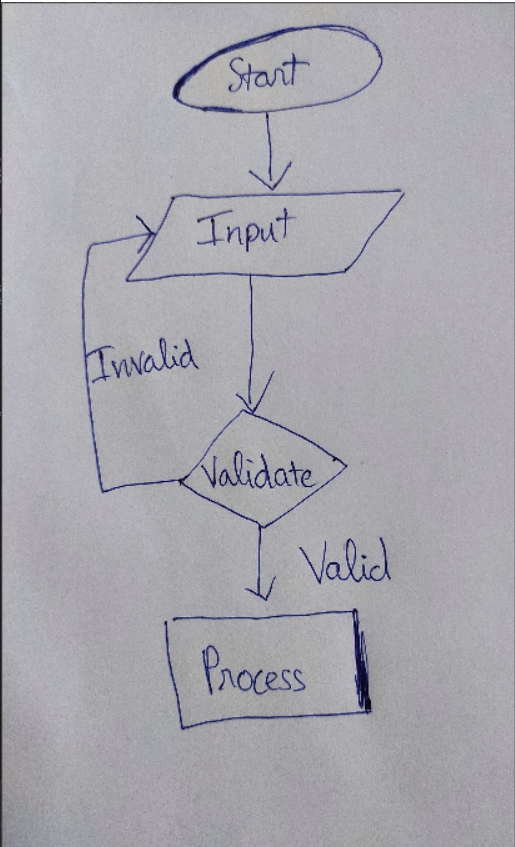
\includegraphics[width=5cm, height=6.5cm]{Images/Preprocessing/rawImage.png}
        \caption{Original Image}
        \label{fig:rawImage}
    \end{subfigure}
    \begin{subfigure}{0.4\textwidth}
        \centering
        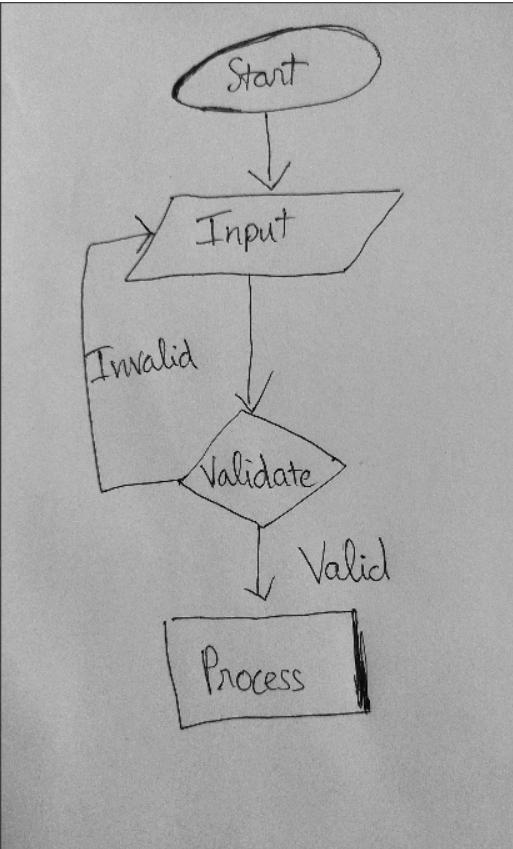
\includegraphics[width=5cm, height=6.5cm]{Images/Preprocessing/grayscale.png}
        \caption{Grayscale image}
        \label{fig:grayscaleImage}
    \end{subfigure}
    \caption{Figure \ref{fig:rawImage} is the original handwriting flow chart; figure \ref{fig:grayscaleImage} is grayscale version of the figure \ref{fig:rawImage}} 
    \label{fig:grayscale_step}
\end{figure}

\subsection{Histogram equalization}
\hspace{0.5cm} {In this step, we use Histogram Equalization technique to improve contrasts in the grayscale image.}

\begin{figure}[h]
    \centering
    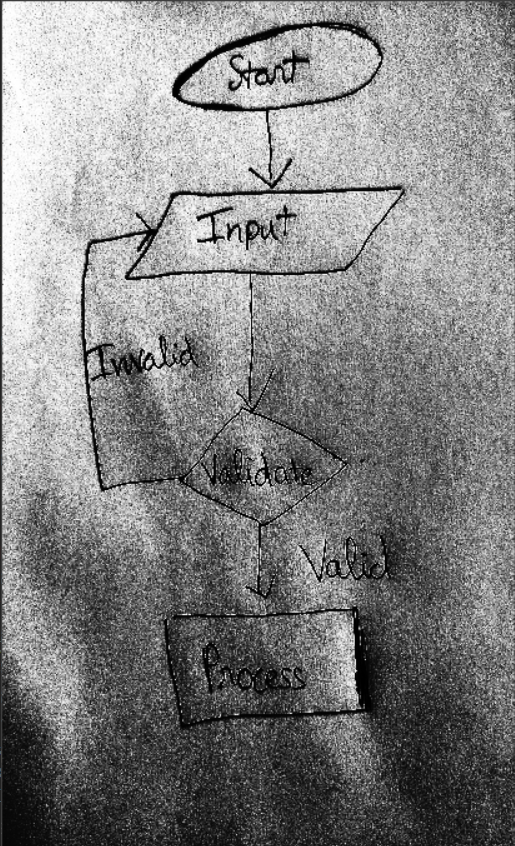
\includegraphics[width=5cm,height=6.5cm]{Images/Preprocessing/histoequal.png}
    \caption{Histogram equalized image converted from figure \ref{fig:grayscaleImage}}
    \label{fig:histoEqualized}
\end{figure}

\begin{figure}[h]
\centering
    \begin{subfigure}{0.4\textwidth}
        \centering
        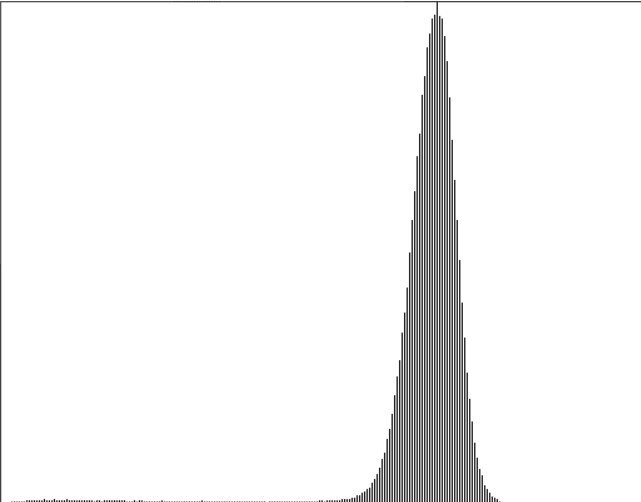
\includegraphics[width=5cm,height=7cm]{Images/Preprocessing/grayhisto.png}
        \caption{Original Histogram}
        \label{fig:origin_histogram}
    \end{subfigure}
    \begin{subfigure}{0.4\textwidth}
        \centering
        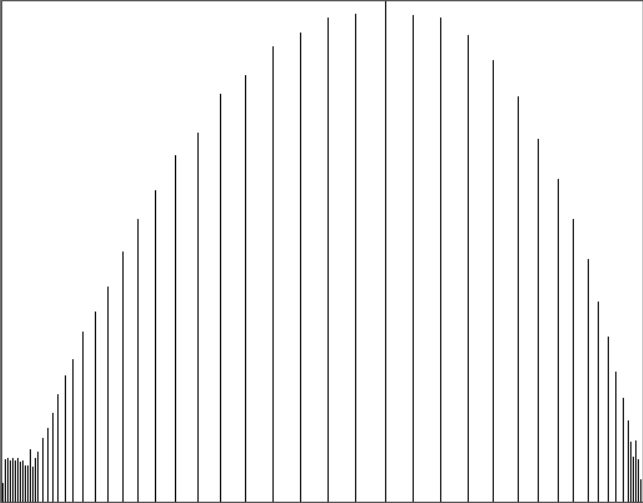
\includegraphics[width=5cm,height=7cm]{Images/Preprocessing/equalhisto.png}
        \caption{Equalized histogram}
        \label{fig:Equalizedhistogram}
    \end{subfigure}
    \caption{Figure \ref{fig:origin_histogram} is the histogram of figure \ref{fig:grayscaleImage}; figure \ref{fig:Equalizedhistogram} } is the figure \ref{fig:origin_histogram} converted to by using Histogram Equalization
    \label{fig:histogram_equalization}
\end{figure}

Observe the figure \ref{fig:histoEqualized}, we can see that this procedure make the image worse than the figure \ref{fig:grayscaleImage}. From the result, we decided to remove the step Histogram Equalization from preprocessing.
\subsection{Image smoothing}
\begin{figure}[h]
    \centering
    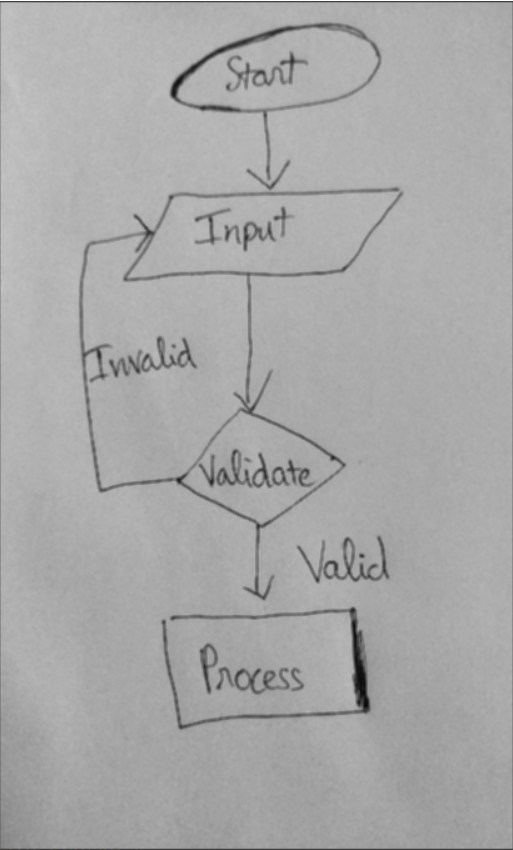
\includegraphics[width=5cm,height=7cm]{Images/Preprocessing/gaussian.png}
    \caption{Gaussian blur applies on \ref{fig:grayscaleImage}}
    \label{fig:gaussian_blur}
\end{figure}
In this step, we filter the noise from the image. As we can see from the figure 6.1 (b), the noise in the figure is Gaussian noise, which represents statistical noise having probability density function equal to the normal distribution, which is also known as the Gaussian distribution. Therefore, to remove this type of noise, Gaussian filter is used in this case. The blurred image after using Gaussian filter is in figure \ref{fig:gaussian_blur}.

\subsection{Convert into binary image}
\begin{figure}[t]
\centering
    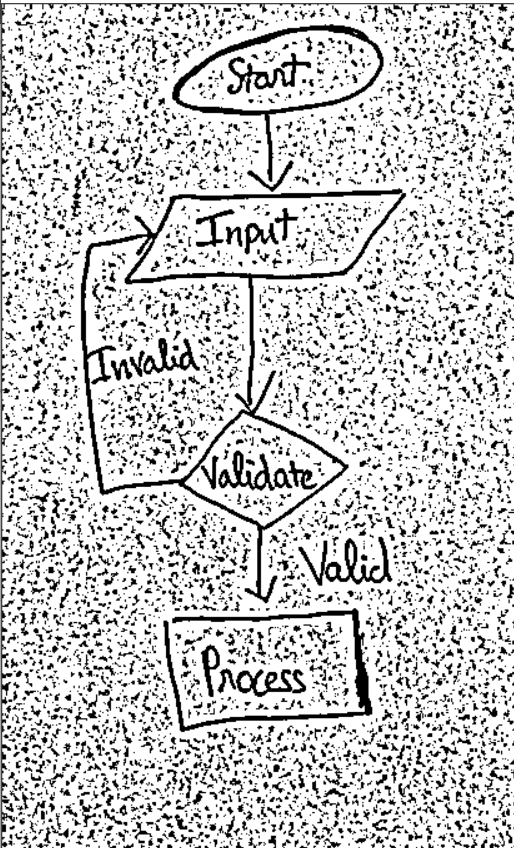
\includegraphics[scale=0.35]{Images/Preprocessing/binaryimage.png}
    \caption{Binary image}
    \label{fig: binary_image}
\end{figure}

In this step, we use the Adaptive Thresholding technique to binarize figure \ref{fig:gaussian_blur}. The result of this step is in figure 6.5. In addition, we also show the result of converting the histogram equalization image, which also is blurred by Gaussian blur, into binary image in this figure. \\

From figure \ref{fig: binary_image}, it can be seen that there are speckle noises which is needed to be removed.

\subsection{Speckle filter}

\begin{figure}[t]
    \centering
    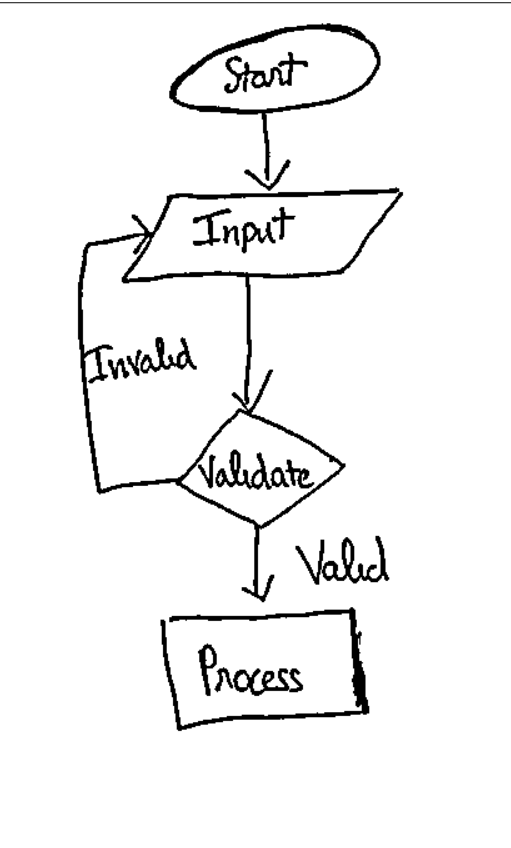
\includegraphics[scale=0.35]{Images/Preprocessing/clearBI.png}
    \caption{Filter speckles in binary image}
    \label{fig:specfilter_BI}
\end{figure}

This is the final step of preprocessing. In this step, we use the filterSpeckles() function from OpenCV to remove the blobs in the binary image. The result we get is in figure \ref{fig:specfilter_BI}.

This function gives a good result with the figure \ref{fig:specfilter_BI}, which separates the flowchart with the black color from the white background.

\section{Web server communication}
This system is designed to transfer images taken from client devices and send them to the web server to process. However, most of the current mobile device has a great camera quality which can produce high definition pictures but also has a large size. Trying to transfer the whole file in one request may cause disruption and corruption of the file. However, the Hypertext Transfer Protocol (HTTP) supports a Multi part Request, which is a combination of one or more sets of data into a single body. The body is then divided into many ''body parts'', each of them has an encapsulation boundary ahead in the combination and the last one is enclosed with a closing boundary \cite{58}. The content-type ''multipart/form-data'' allows the app to send the image by blocks of data, which will then be collected by the web server.

Flutter HTTP package supports multipart/form-data requests. When this request is called, it automatically sets the Content-Type header to multipart/form-data. This value will override any value set by the user. There are many ways to perform this request, in this experiment, we used MultipartFile.fromBytes, which will create a new multi part file from a byte array. That means first the image needs to be converted into a list of bytes, then will be transformed into a multipart file and send over (see Figure \ref{fig:ImageSendClient}). The web server will receive the file as a stream (see Figure \ref{fig:ImageSendServer}).

\begin{figure}[!b]
\centering
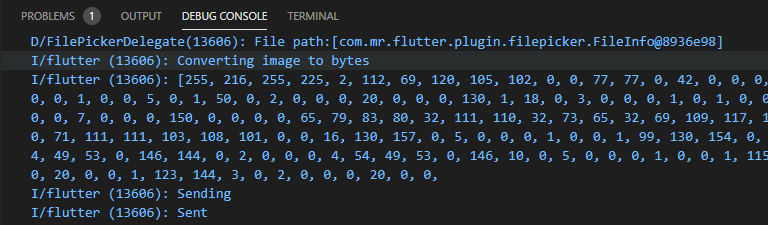
\includegraphics[width=14cm]{Images/App/ImageSendClient.png}
\caption{Client application sending image log}
\label{fig:ImageSendClient}

\centering
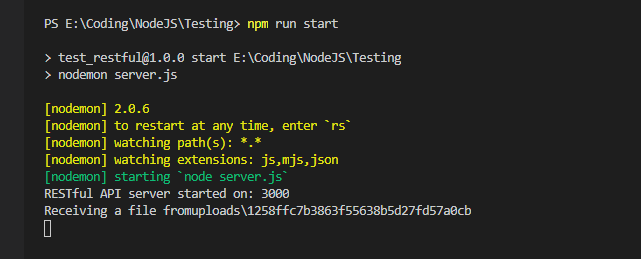
\includegraphics[width=14cm]{Images/App/ImageSendServer.png}
\caption{Server log}
\label{fig:ImageSendServer}
\end{figure}

\section{Display diagram on device}
\subsection{Interactive Viewer and Matrix4}
In order to handle user action like panning, zooming and moving around the diagram, the surface that used to draw the diagram on need to be interactive. One of the most powerful widget (all components in Flutter is fundamentally defined as a widget) in Flutter is the transform class widget which is able to change the perspective of the user of a widget. Basically it makes changes in how the widget look and behave so that developer can create new and more complex component from the existed one. It is controlled by a four dimensions matrix that define how the widget will transform called ''matrix4''. While Flutter also provides other easier ways for scaling, rotating and translating, ''matrix4'' allows more customization. ''Interactive Viewer'' is one of the widget created from the transform class that allows user to transform all the components inside by dragging to pan or pinching to zoom. The difference of it from the rest is it can create a wide space for interacting and is mainly used to grab the widgets that is too big to fit inside the screen, which is a perfect space to draw the diagram on. ''Interactive Viewer'' transforms itself by changing some specific value in the ''matrix4''.

For example, in the table \ref{fig:matrix4}, we can see a 4x4 matrix represent the ''matrix4'', by default it is an identity matrix (which has all the value in the diagonal line equal to 1). In that state, the widget is in its normal size (see Figure \ref{fig:defaultspace}). Then it can  be tweeted in order to achieve the prefer shape.

To scale the widget (change its size to make it bigger or smaller): we can change the value ''a'' and ''b'' in the table \ref{fig:matrix4} into a value greater than zero (zero value will make the matrix unable to reverted ). Value smaller than one will make it shrink and value greater than one will expand it in the corresponding dimension. In the table, value ''a'' controls the X-dimension or the width of the space (see Figure \ref{fig:xscale}) and ''b'' does the same for the height (Y-dimension) (see Figure \ref{fig:yscale}).

In a two dimension perspective, that maybe enough to express most of the form of the space. However, there is also the value ''c'' that may influence the way user interact with the space, which scaling in the Z-dimension. For instance, in Figure \ref{fig:zscaledemo}, value ''c'' in position 3,3 has been changed to 2.0 but the space remain unchanged. In theory, the Z-dimension represents how deep the widget should look like, then it may seem to be unnecessary in a 2D space, but as it is zoomed out (see Figure \ref{fig:zoomzscale}) then the zooming scale has been increased, as if the widget is now further from the screen perspective.

Finally, The space can be moved the space around in X and Y dimension by changing value in ''d'' (4,1) and ''e'' (4,2) position. Value in this position will be consider as the amount of pixels that the space move. For example, in Figure \ref{fig:xmove}, ''d'' is set to 100, that means the space will move right 100 pixels. The same thing with Figure  \ref{fig:ymove} with ''e'' equals 100, the space will move down 100 pixels.

\subsection{Result}
After applying the previous widget and display the symbol and line with a stack in the diagram space, we get the result as show in figure \ref{fig:result}.


\begin{figure}[t]
    \centering
    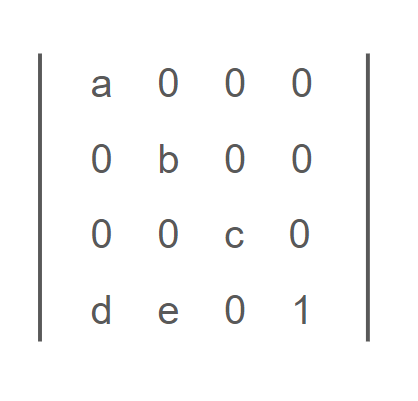
\includegraphics[width=8cm]{Images/App/matrix4.png}
    \caption{Example of matrix4}
    \label{fig:matrix4}
\end{figure}

\begin{figure}[b]
    \begin{subfigure}{0.4\textwidth}
        \centering
        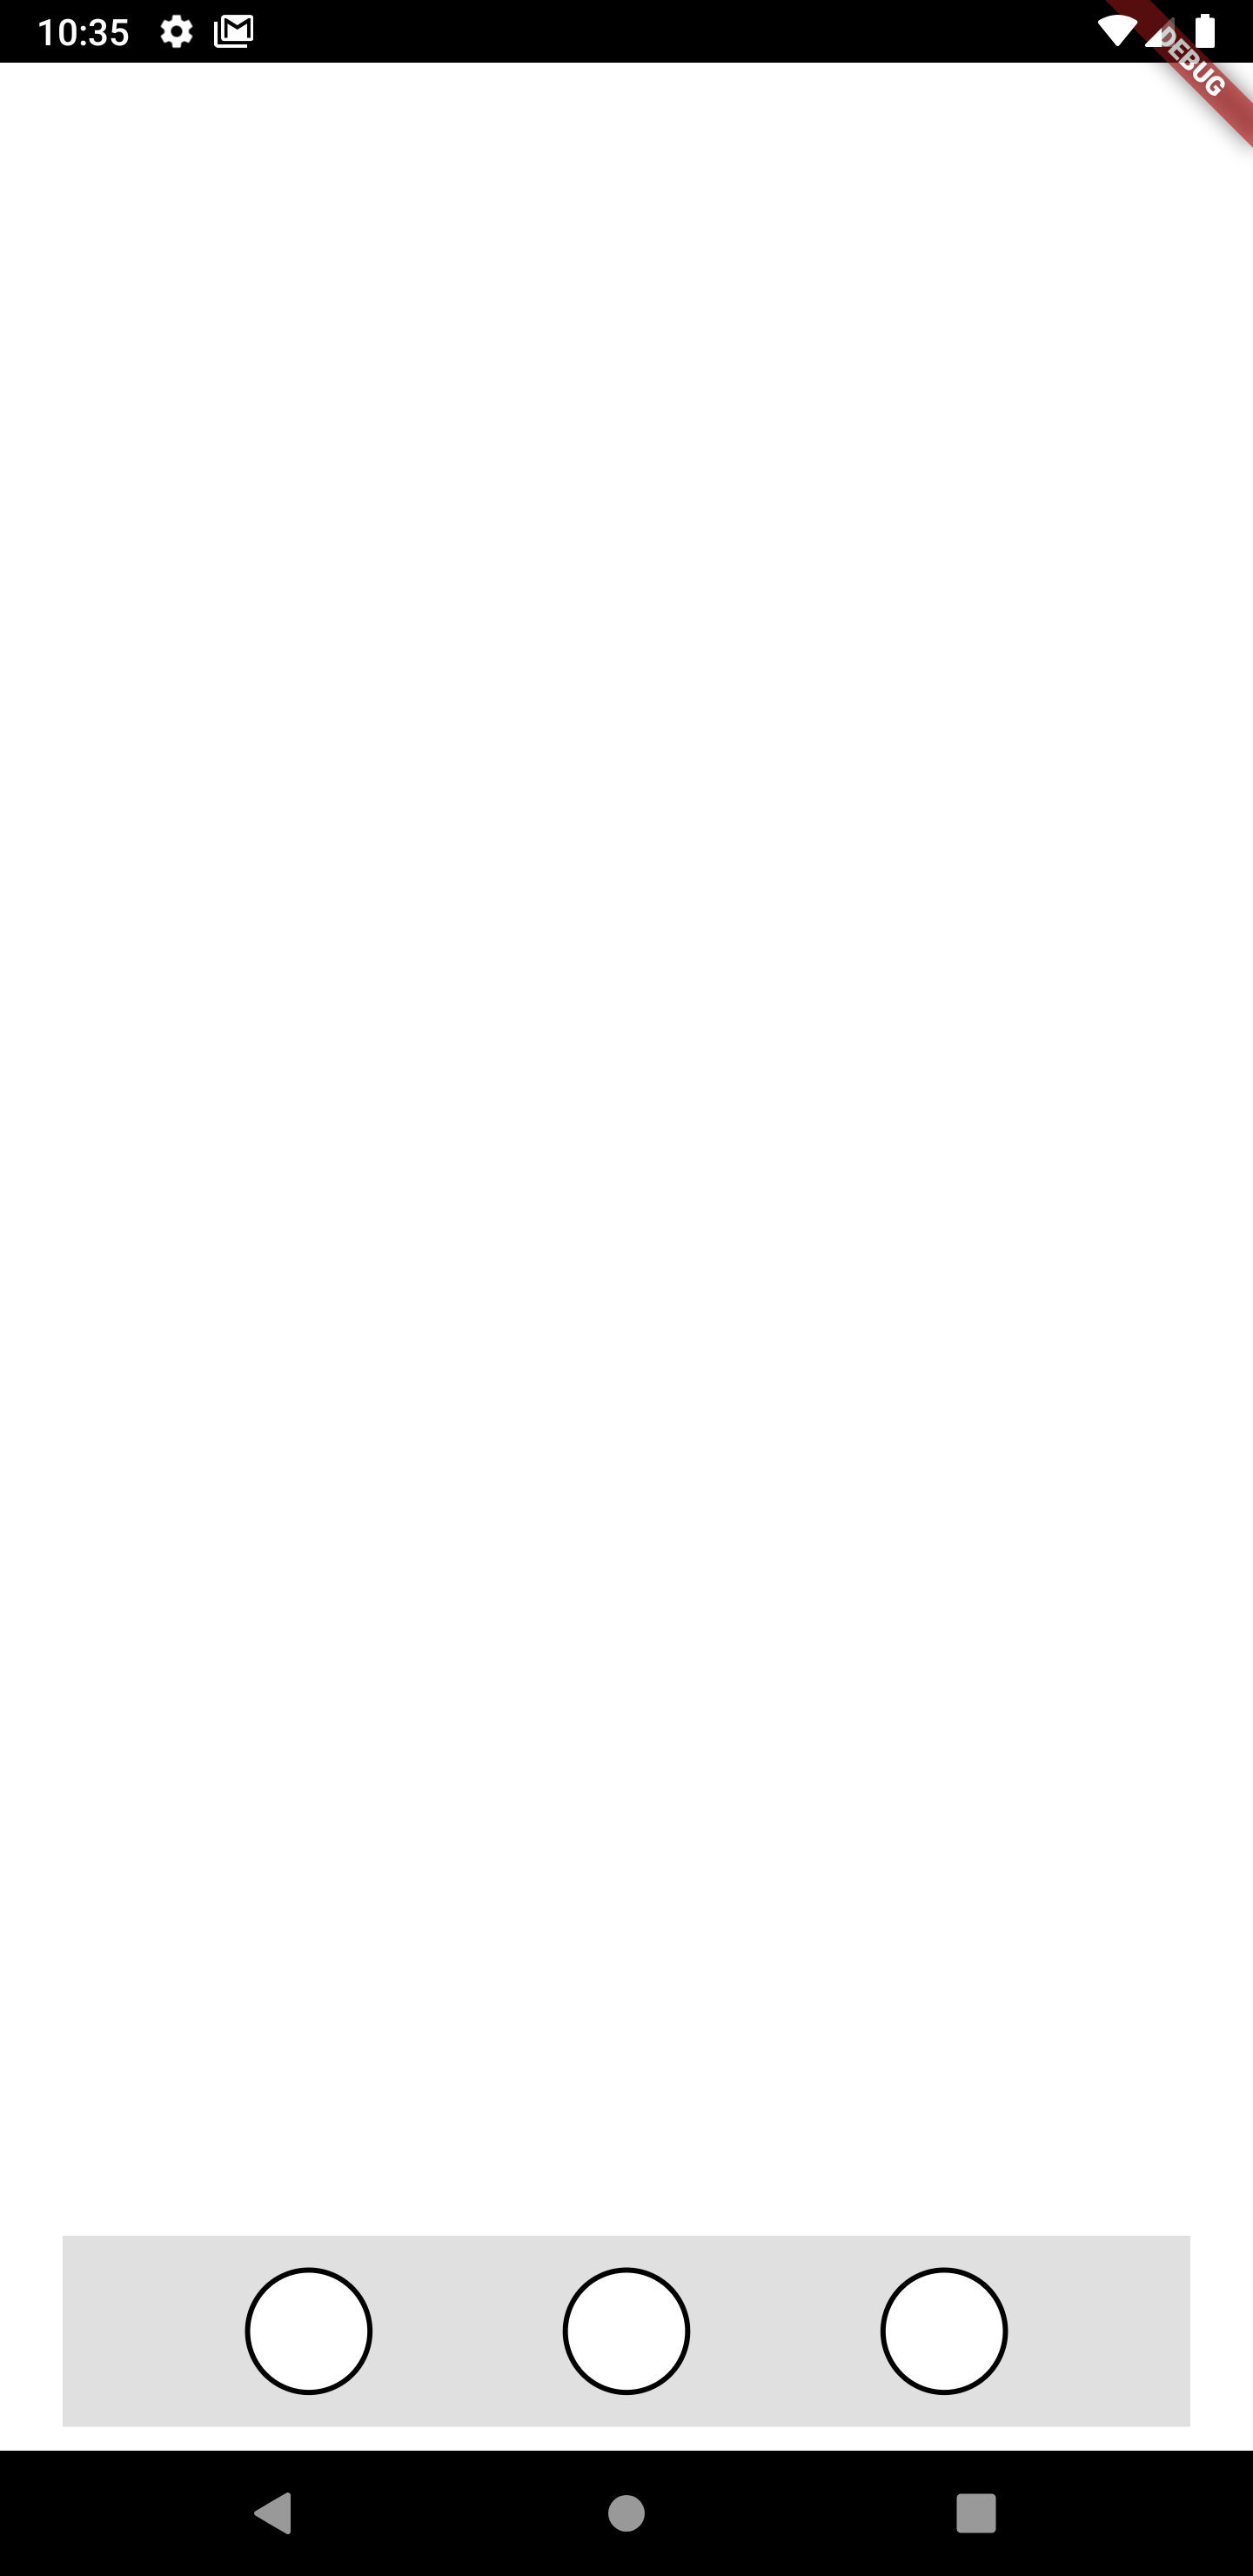
\includegraphics[width=5cm]{Images/App/fullspace.png}
        \caption{Default}
        \label{fig:fullspace}
    \end{subfigure}
    \hfill
    \begin{subfigure}{0.4\textwidth}
        \centering
        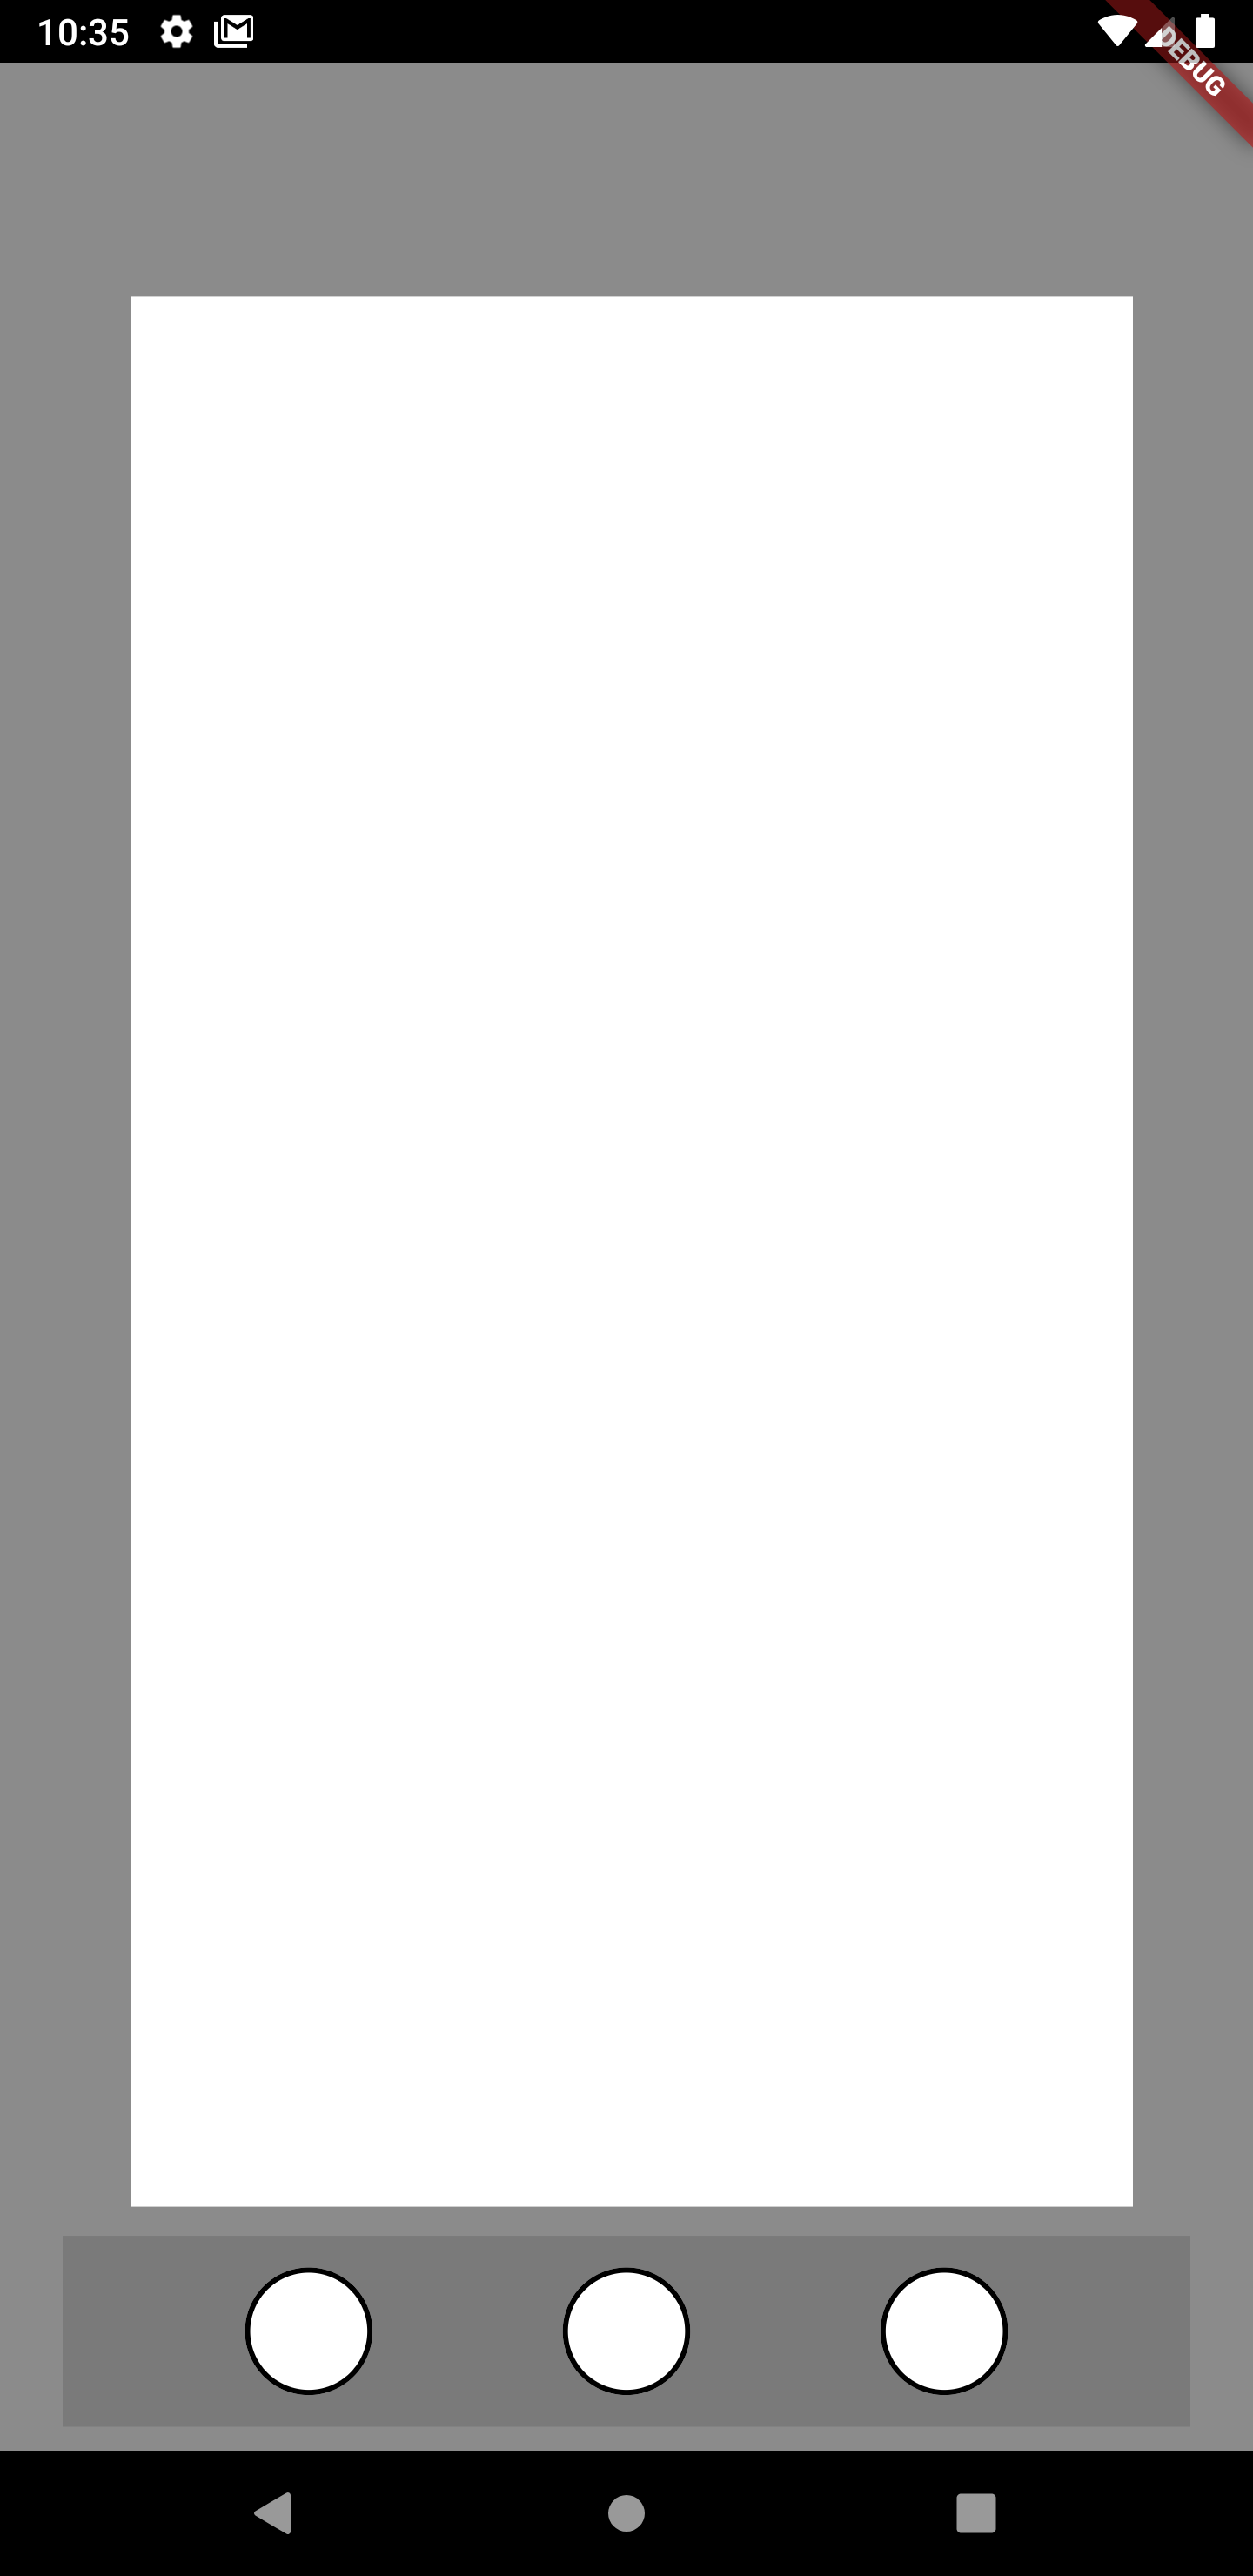
\includegraphics[width=5cm]{Images/App/fullzoom.png}
        \caption{Zoom out from the default}
        \label{fig:fullzoom}
    \end{subfigure}
    \caption{Interactive space using identity matrix}
    \label{fig:defaultspace}
\end{figure}

\begin{figure}[b]
    \begin{subfigure}{0.4\textwidth}
        \centering
        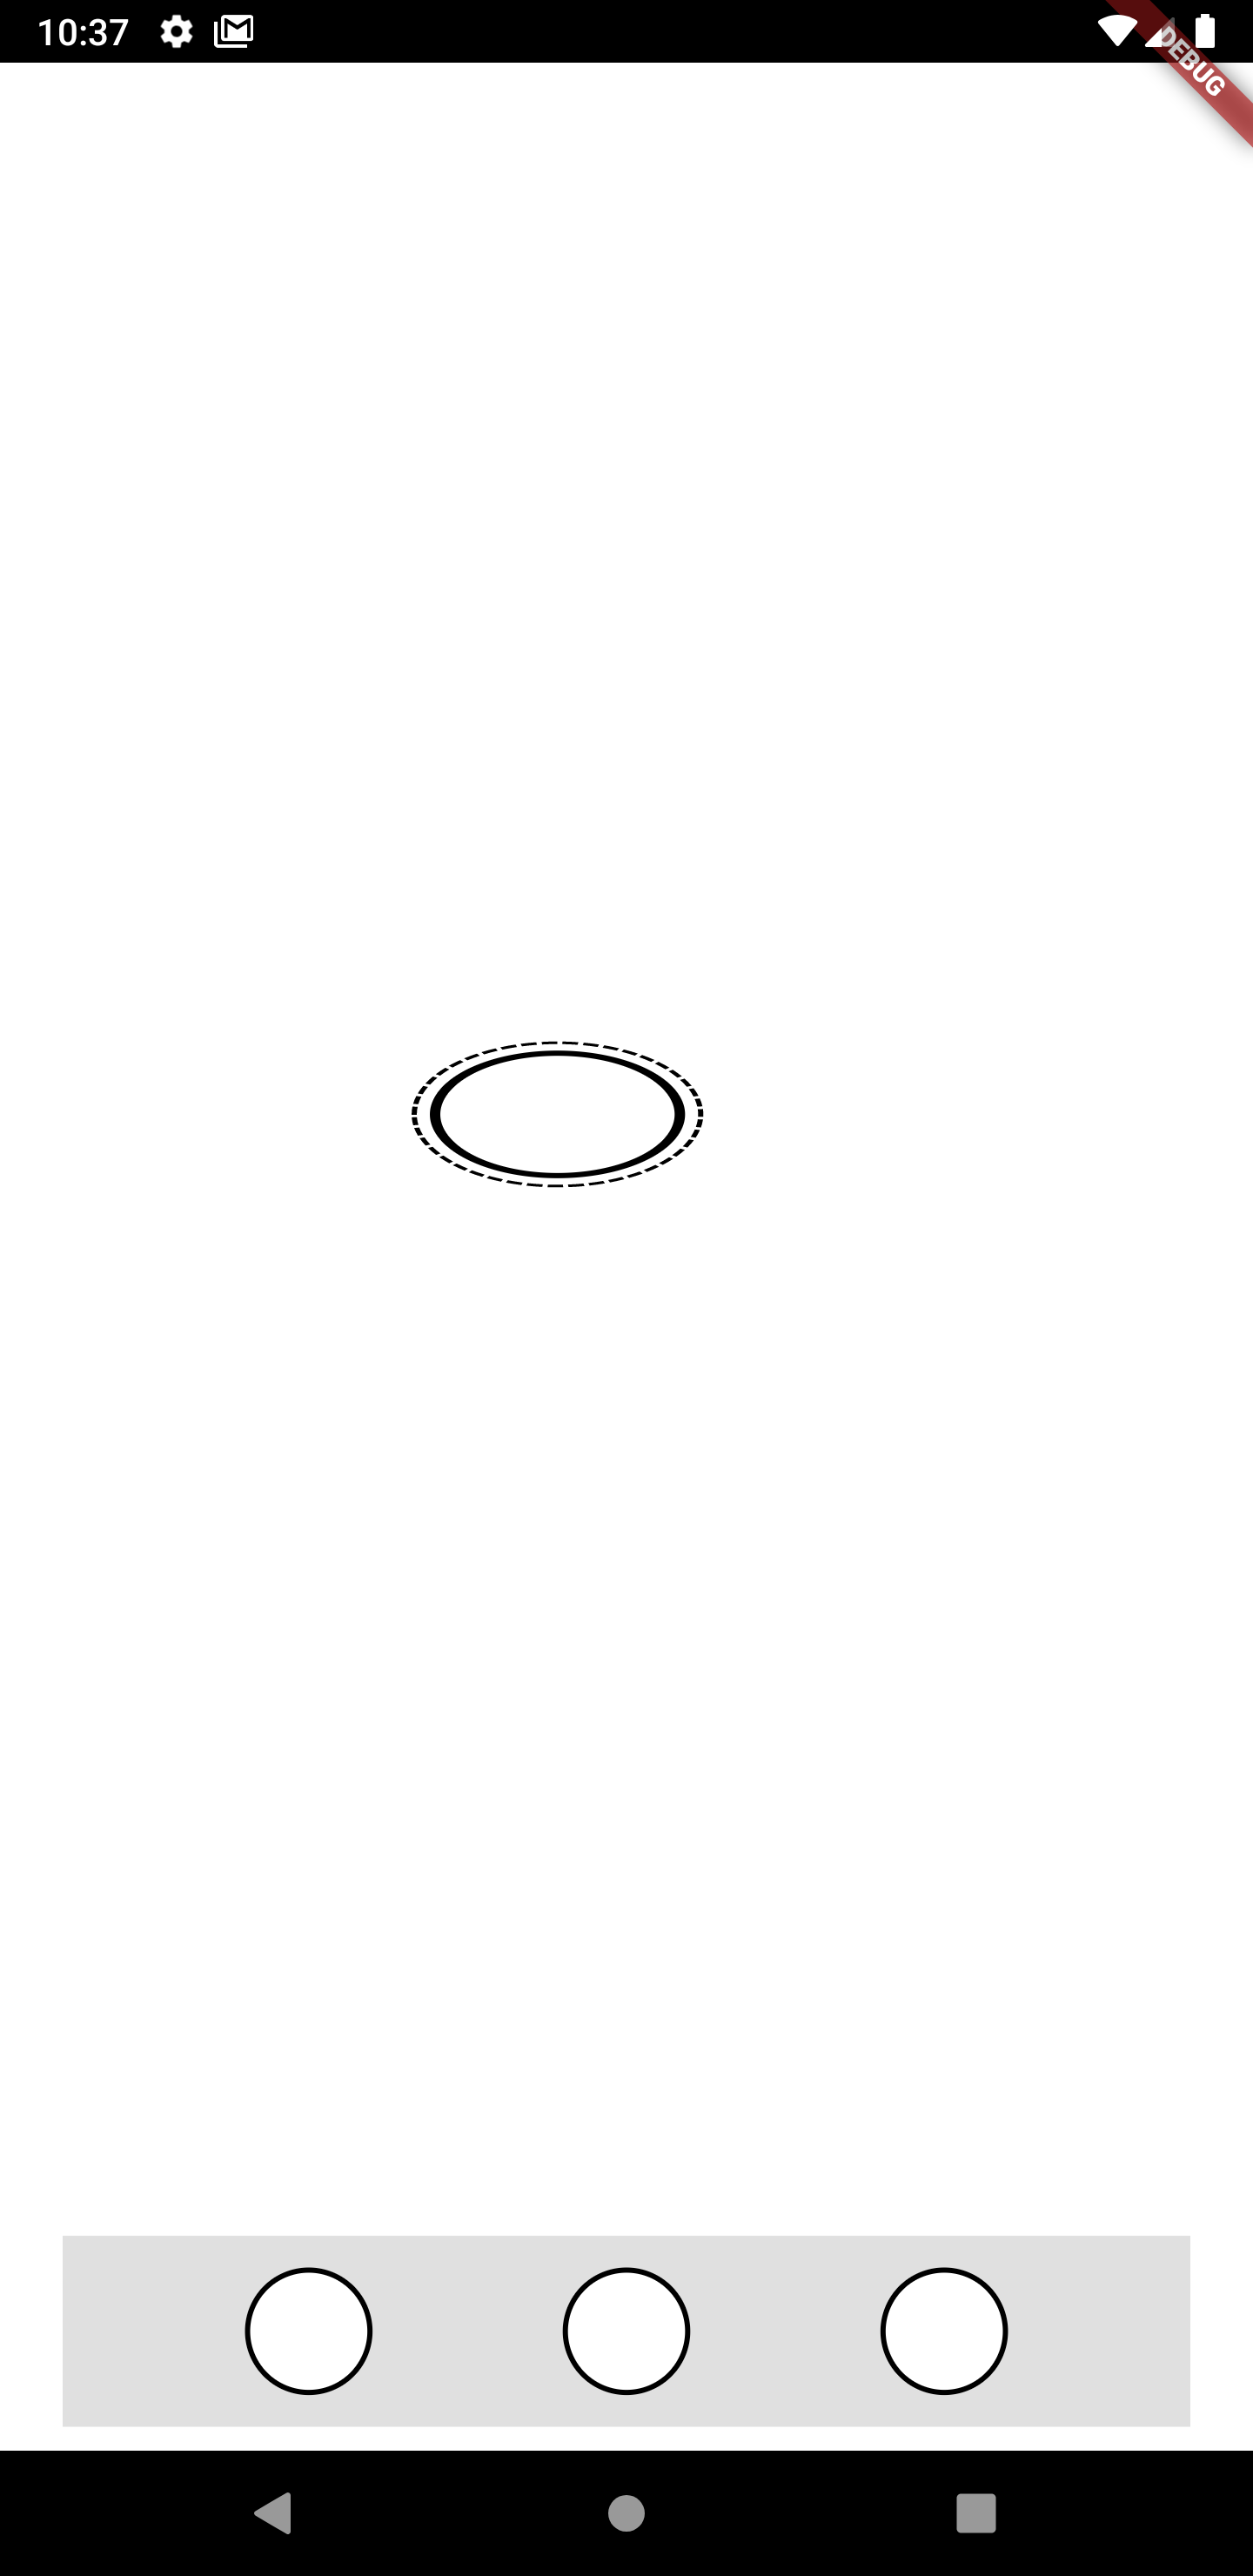
\includegraphics[width=5cm]{Images/App/xscale.png}
        \caption{Value a (1,1) = 2.0}
        \label{fig:xscale}
    \end{subfigure}
    \hfill
    \begin{subfigure}{0.4\textwidth}
        \centering
        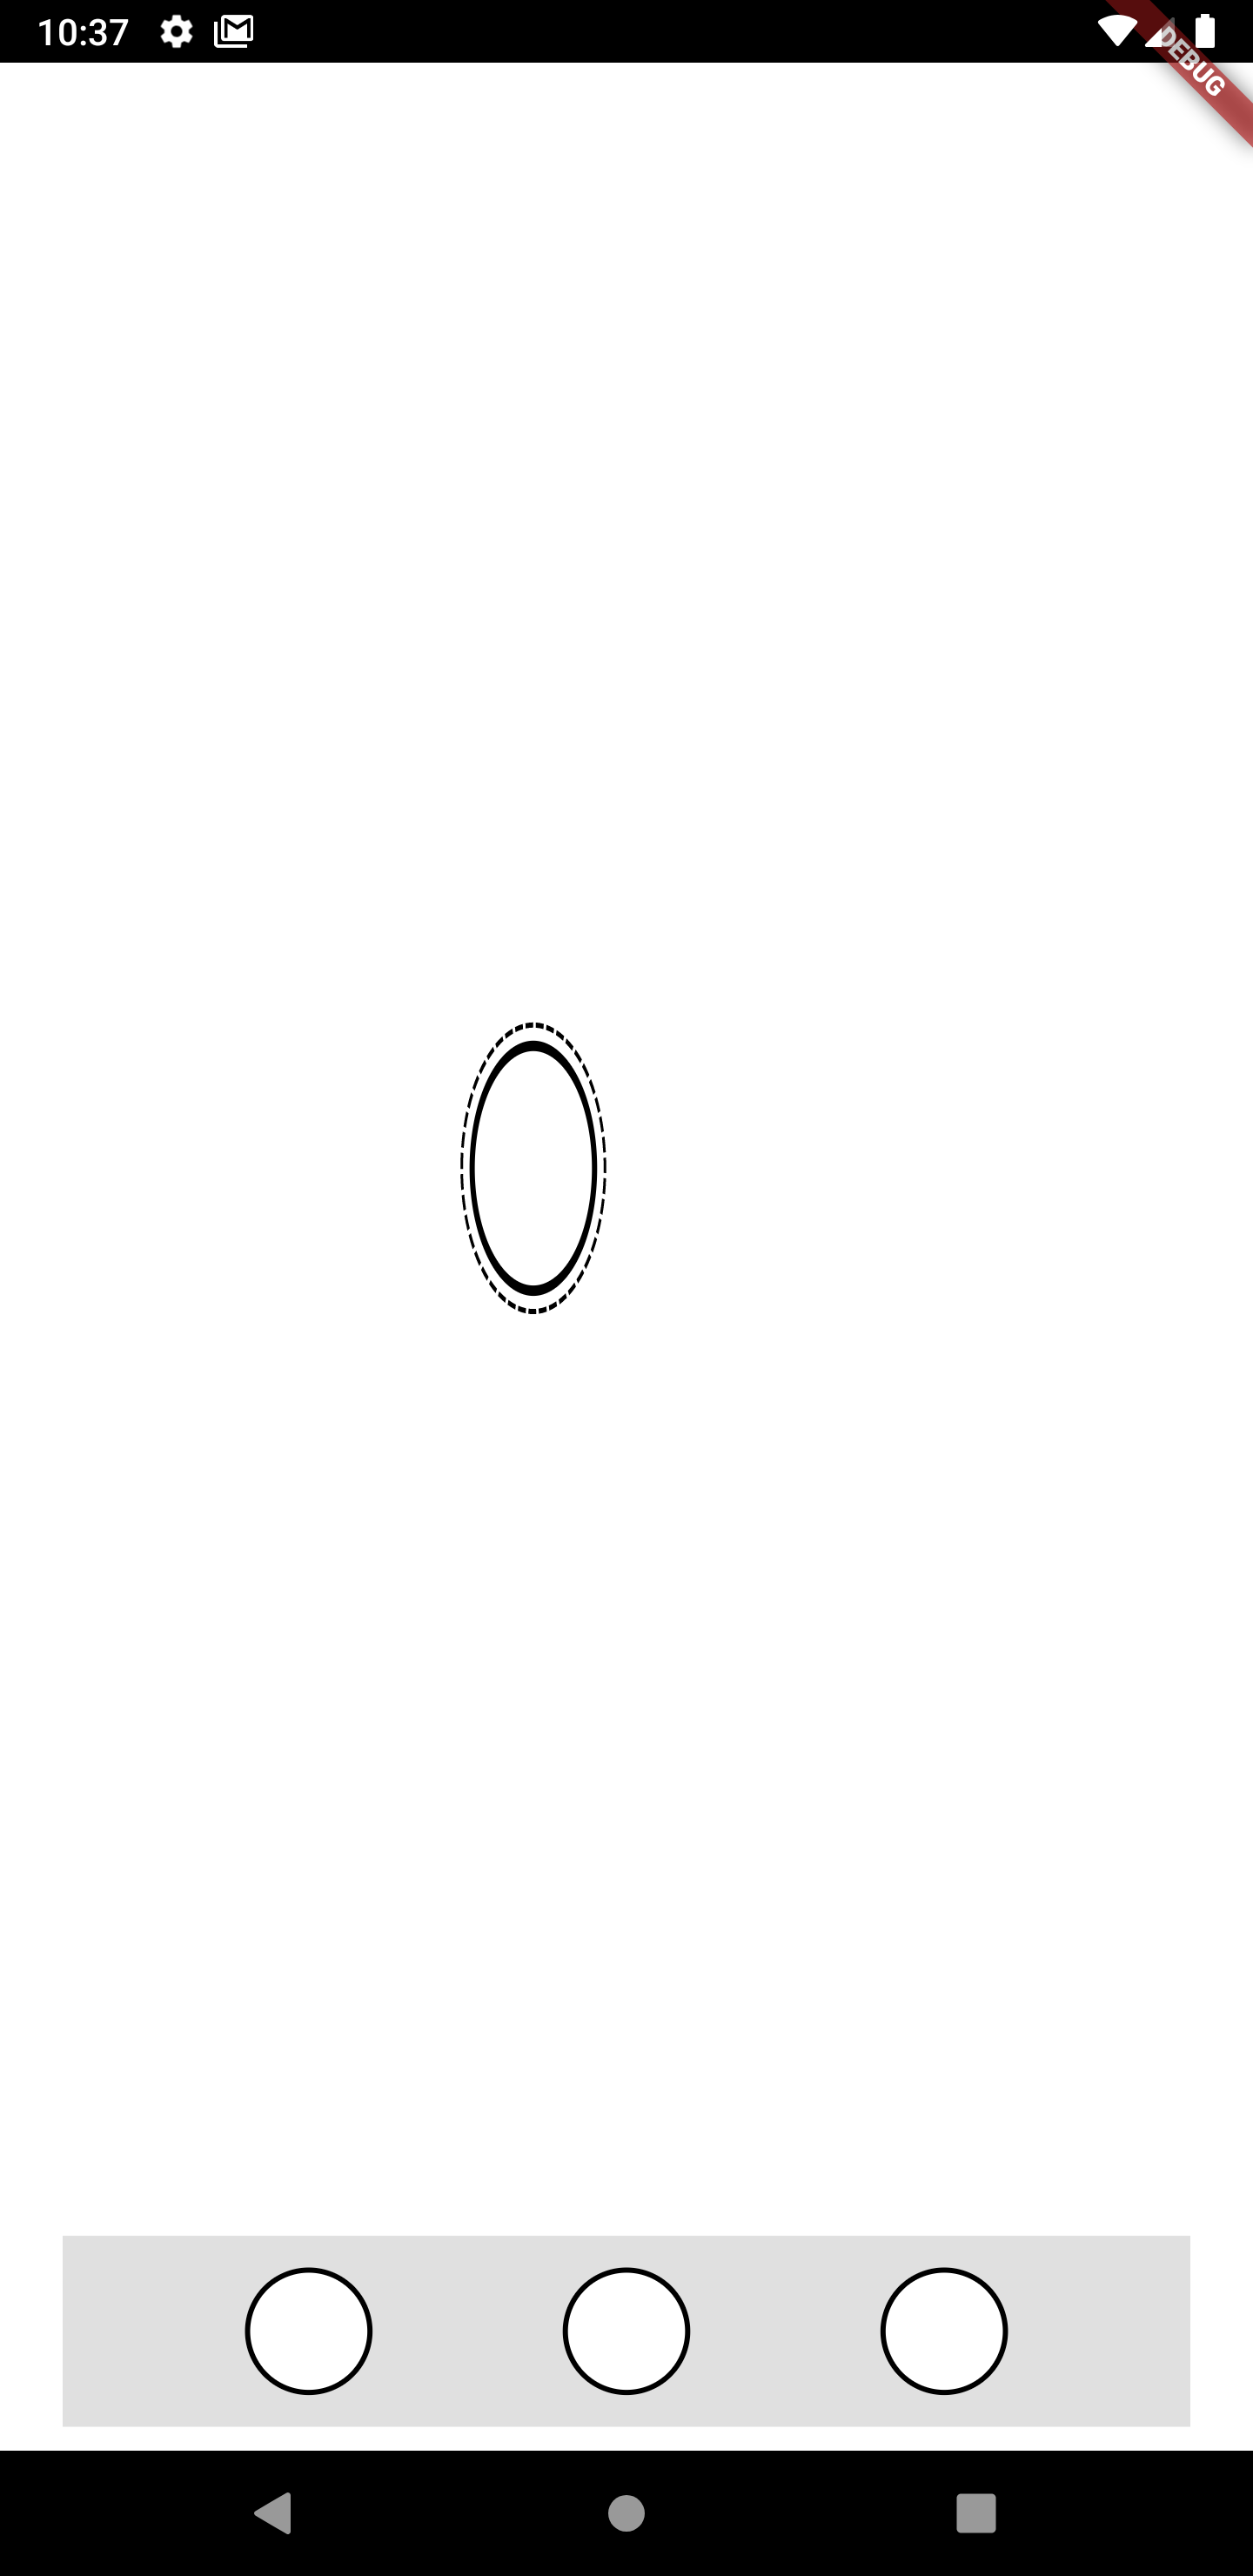
\includegraphics[width=5cm]{Images/App/yscale.png}
        \caption{Value b (2,2) = 2.0}
        \label{fig:yscale}
    \end{subfigure}
    \caption{Scaling in X and Y}
    \label{fig:xysacle}
\end{figure}

\begin{figure}[b]
    \begin{subfigure}{0.4\textwidth}
        \centering
        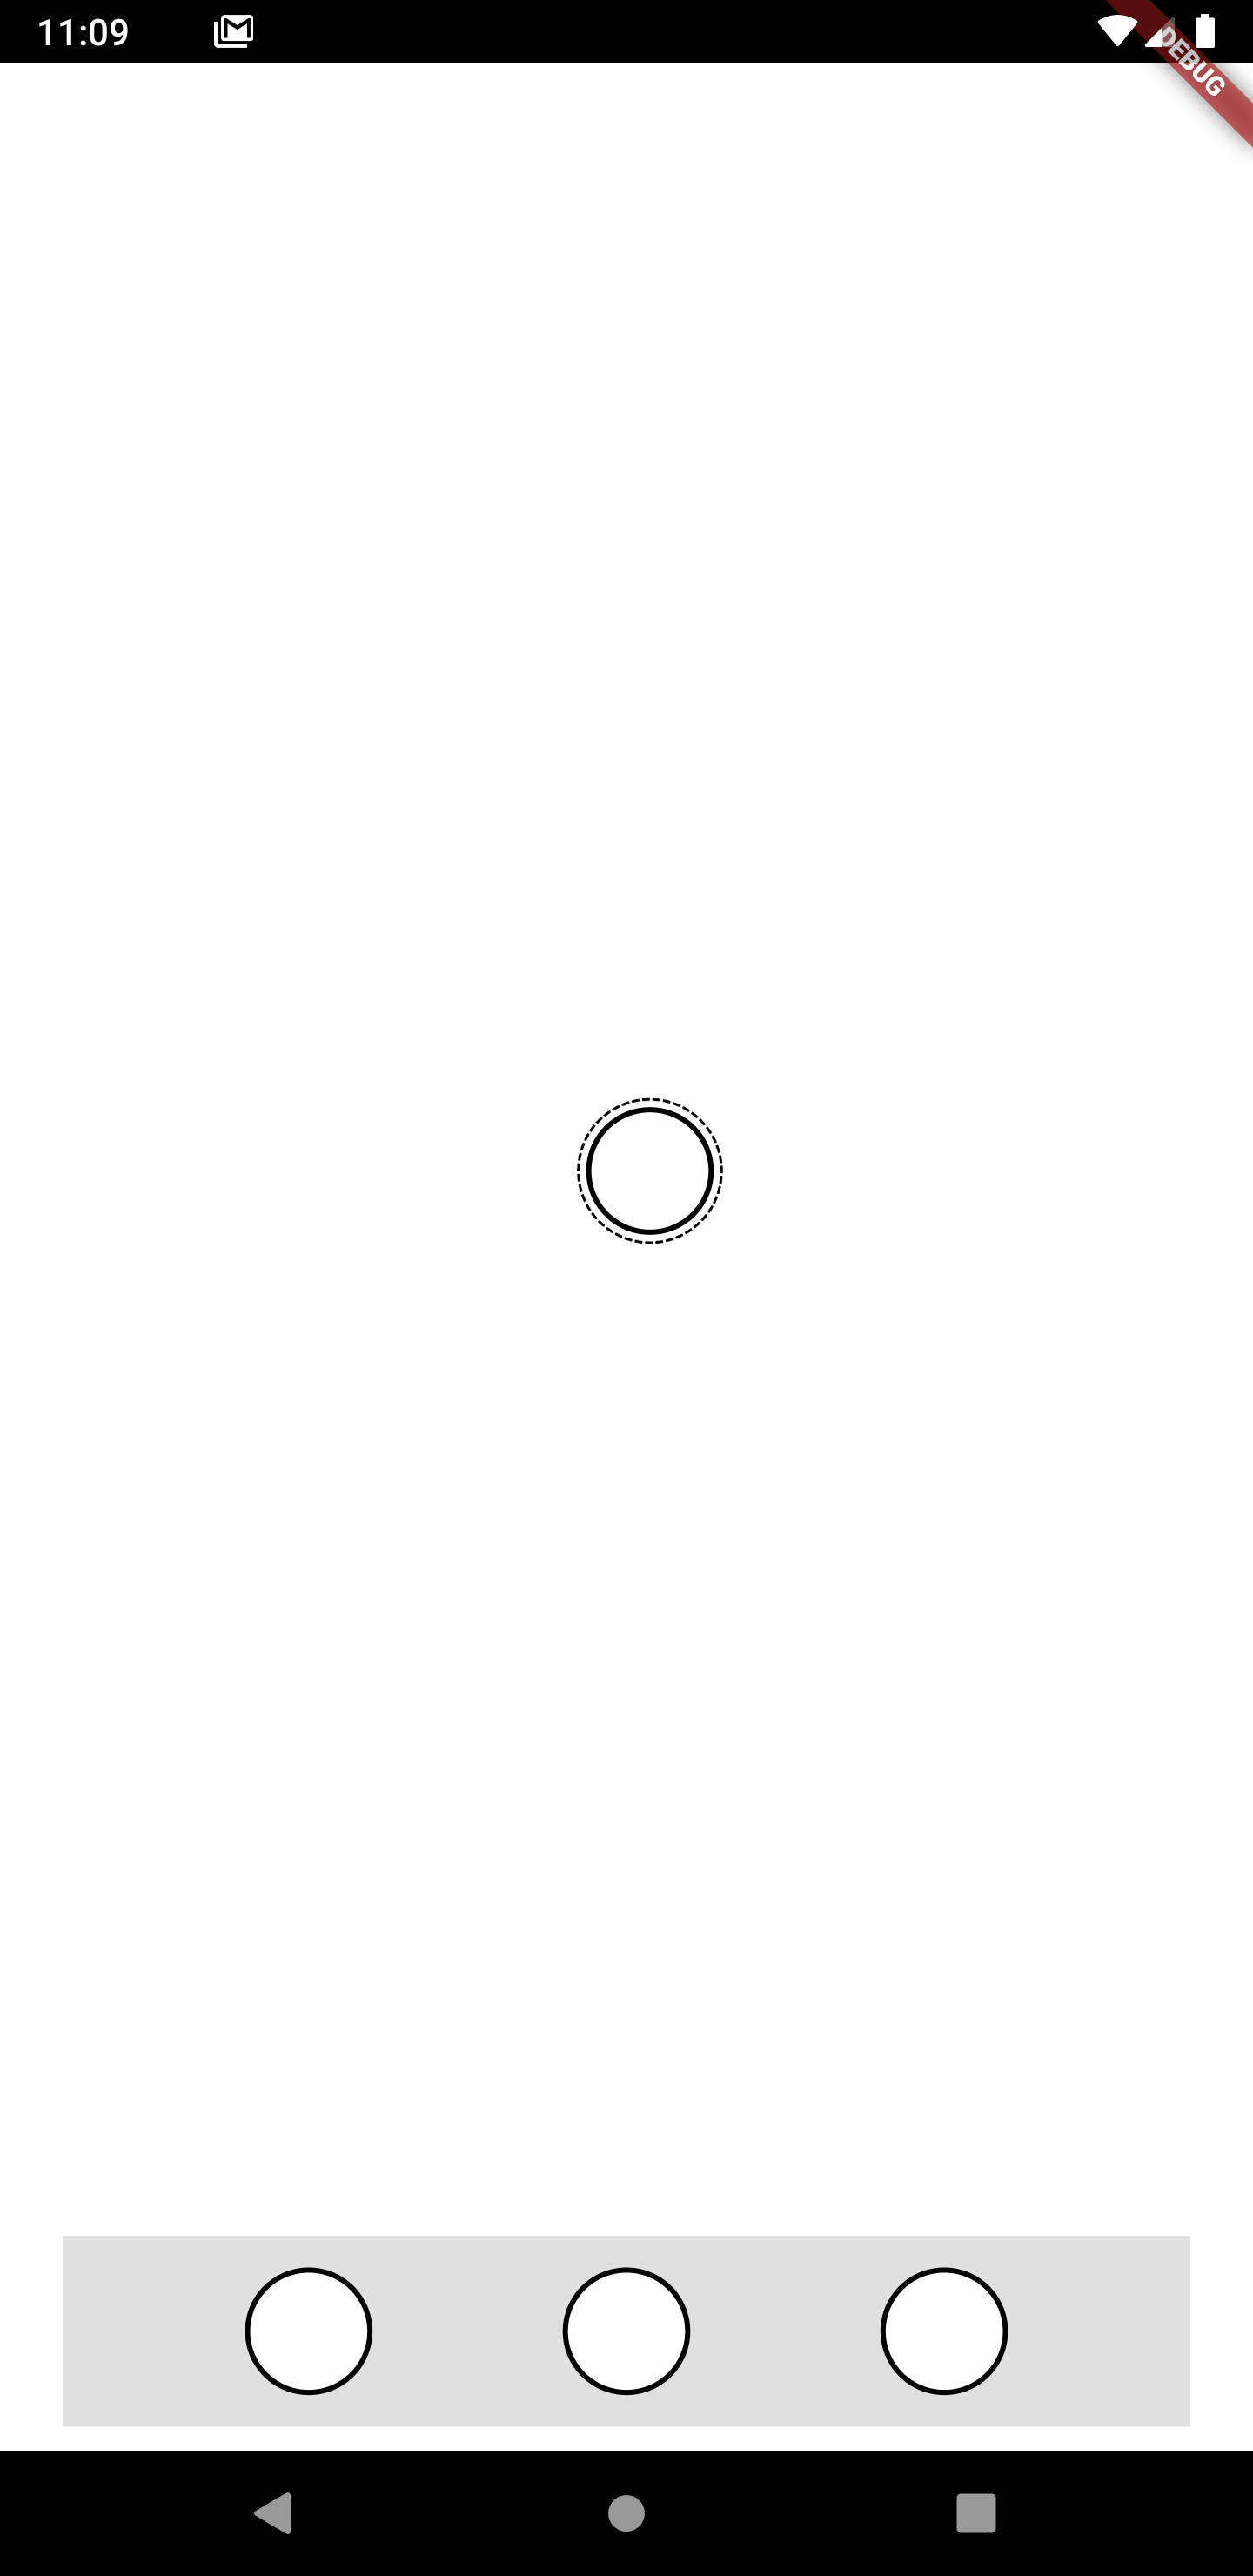
\includegraphics[width=5cm]{Images/App/zscale.png}
        \caption{Value c (3,3) = 2.0}
        \label{fig:zscaledemo}
    \end{subfigure}
    \hfill
    \begin{subfigure}{0.4\textwidth}
        \centering
        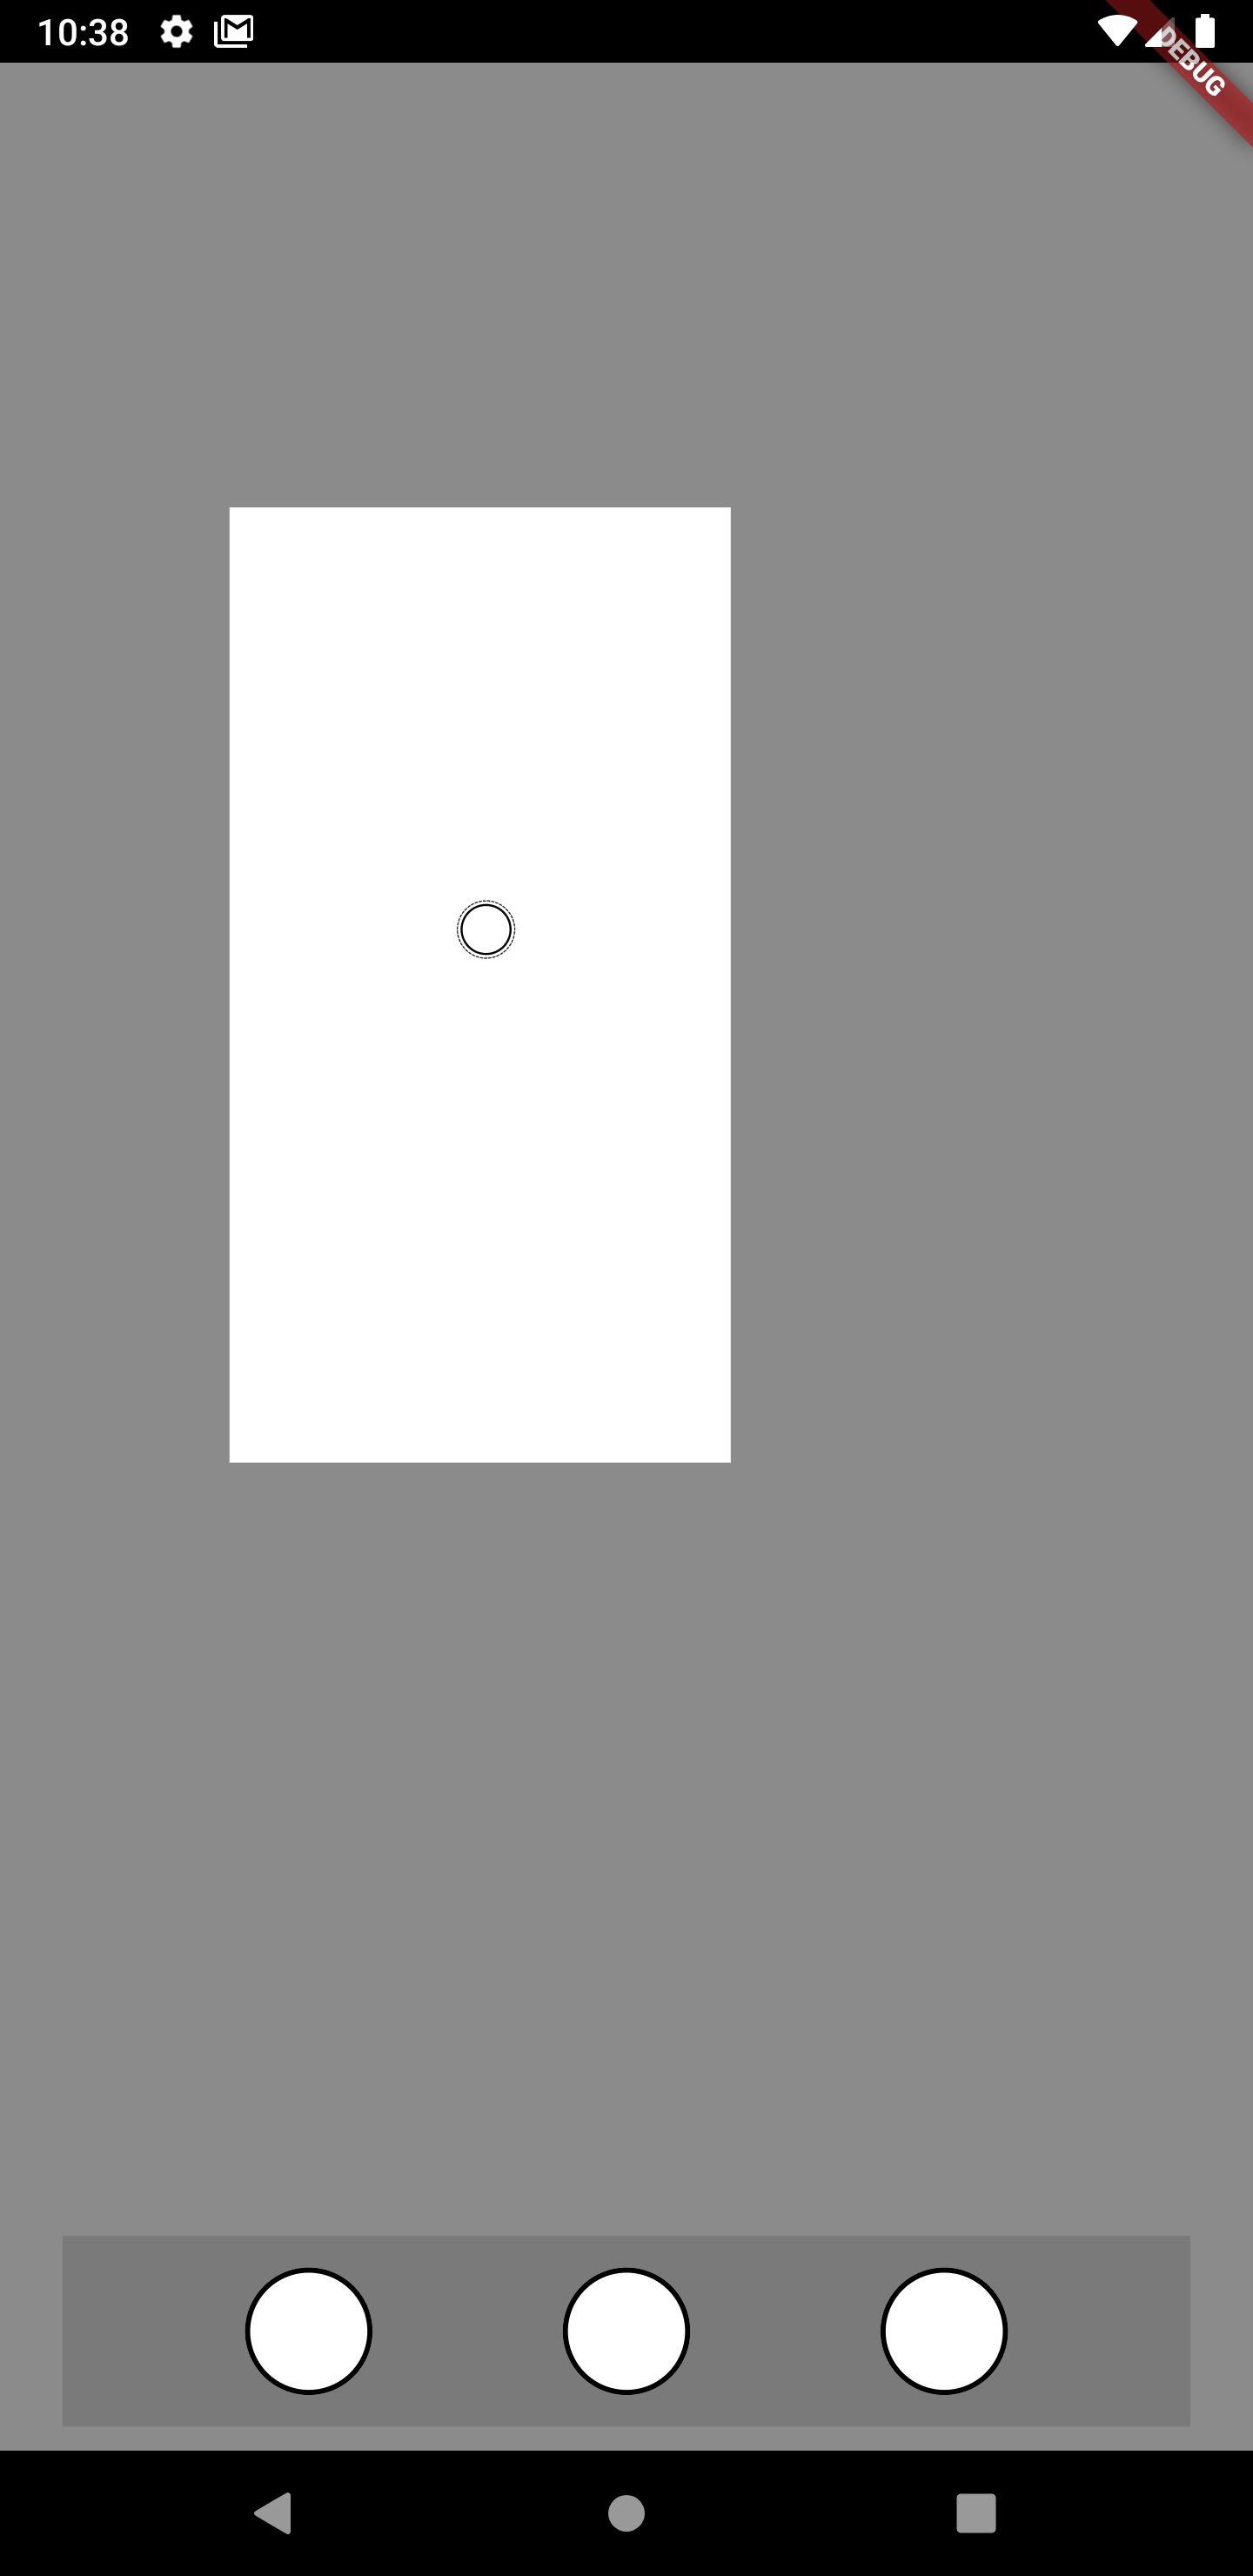
\includegraphics[width=5cm]{Images/App/zoomzscale.png}
        \caption{Zoom out with c = 2.0}
        \label{fig:zoomzscale}
    \end{subfigure}
    \caption{Scaling in Z}
    \label{fig:zscale}
\end{figure}

\begin{figure}[b]
    \begin{subfigure}{0.4\textwidth}
        \centering
        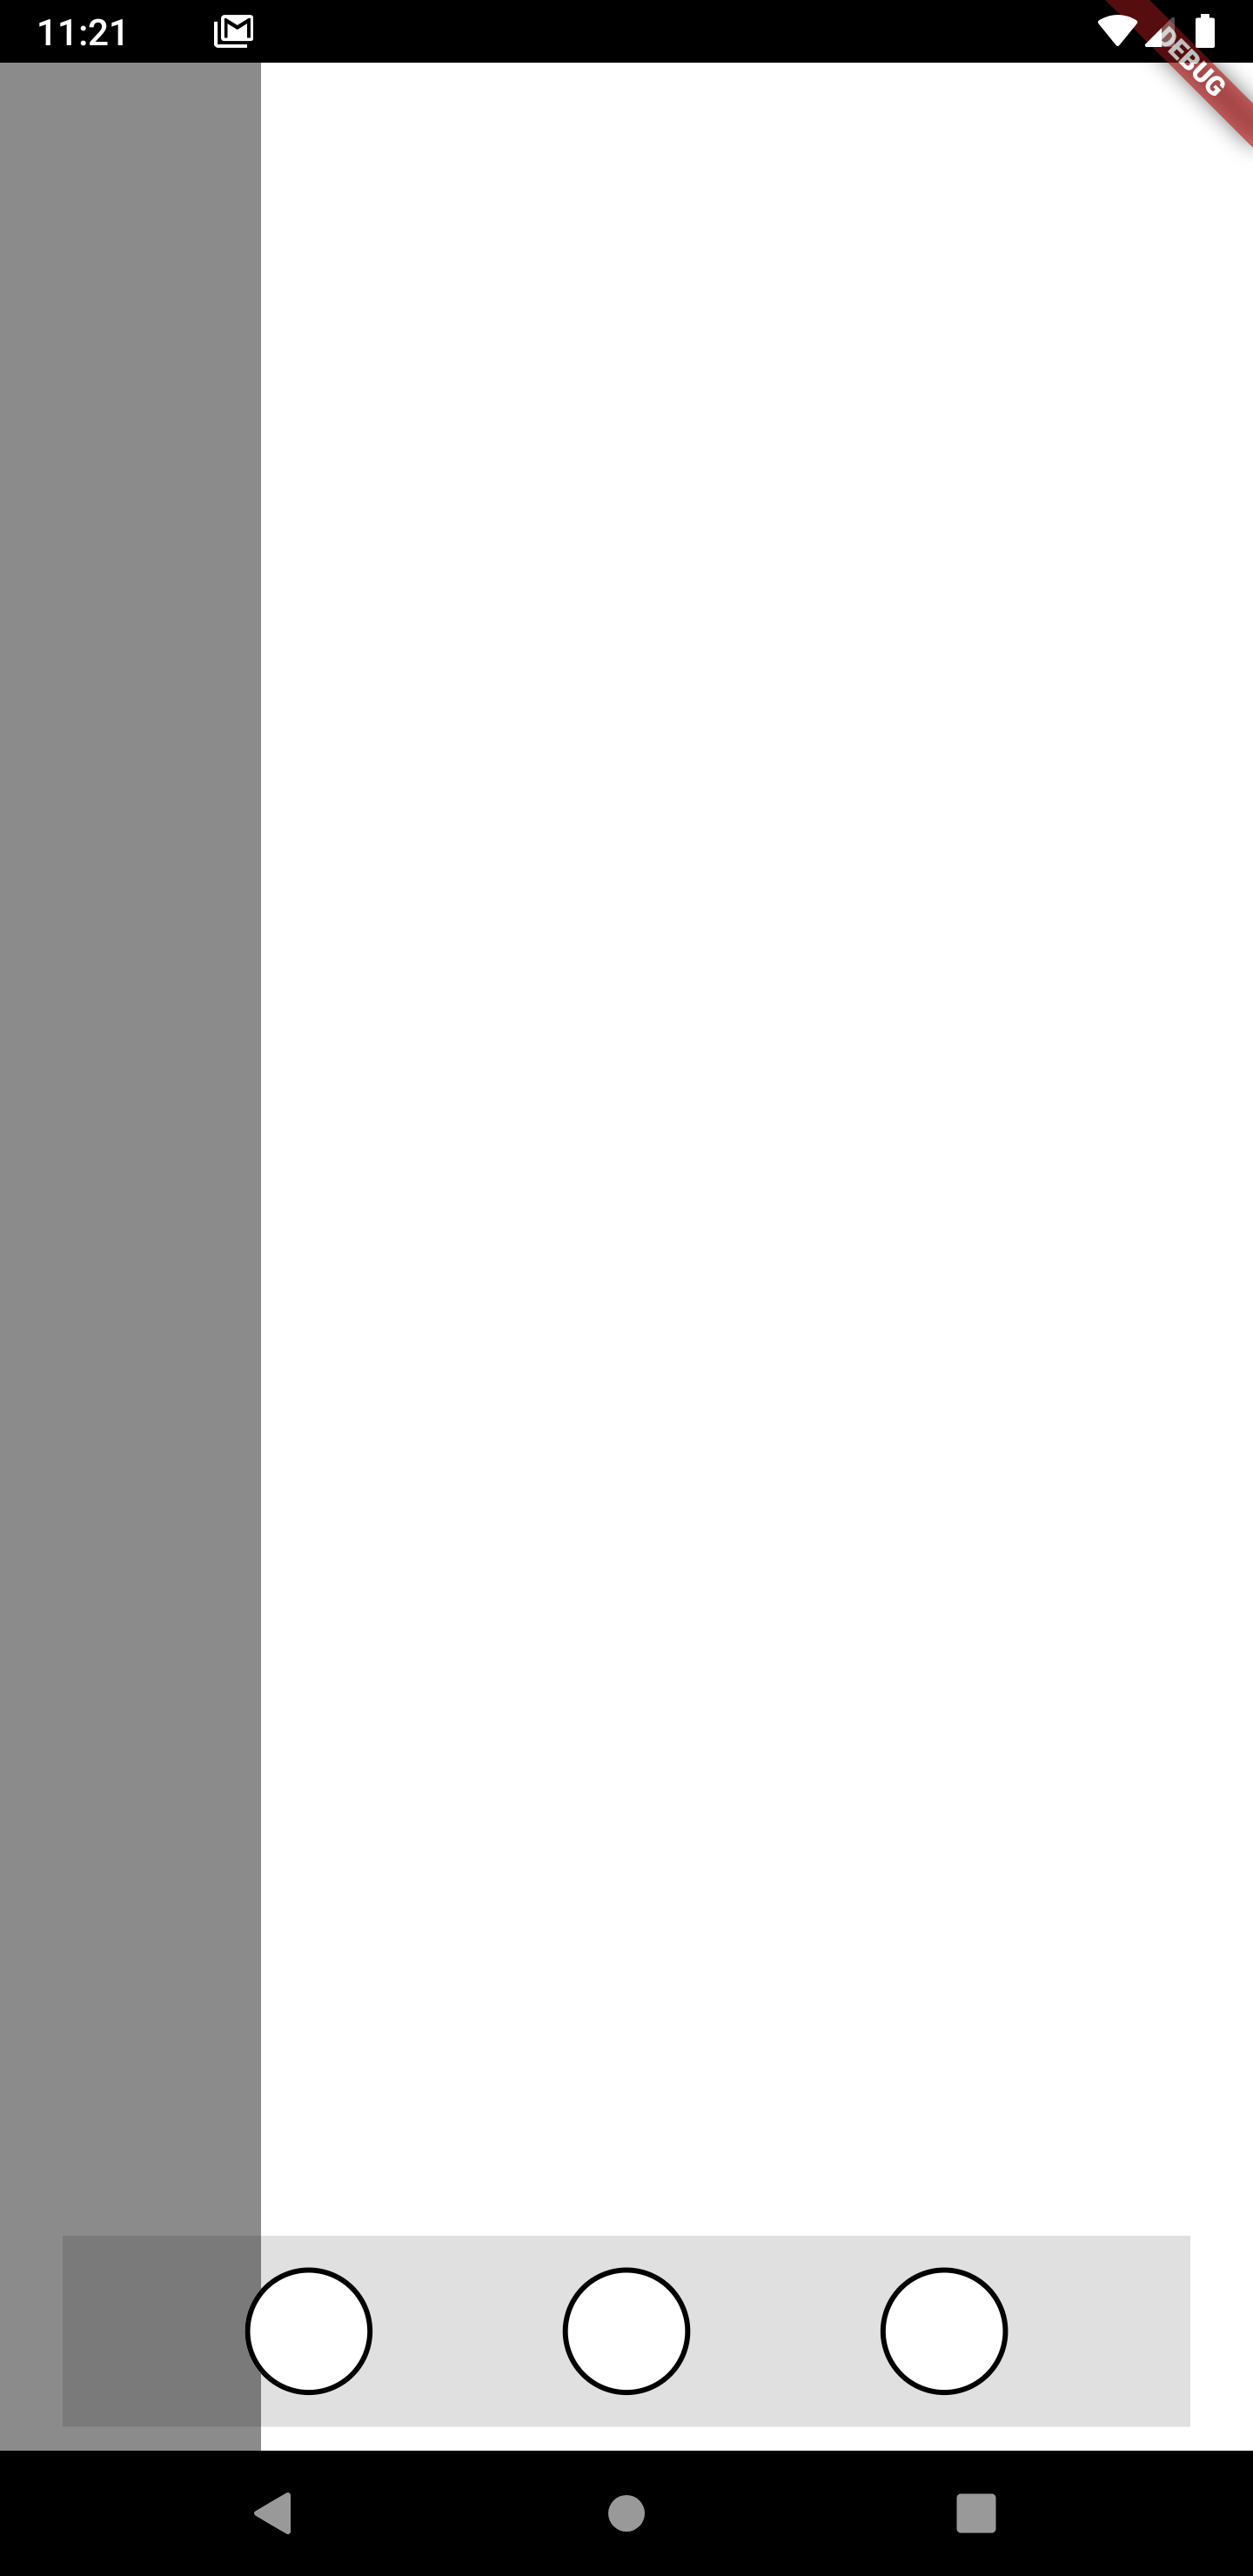
\includegraphics[width=5cm]{Images/App/xmove.png}
        \caption{Value d (4,1) = 100}
        \label{fig:xmove}
    \end{subfigure}
    \hfill
    \begin{subfigure}{0.4\textwidth}
        \centering
        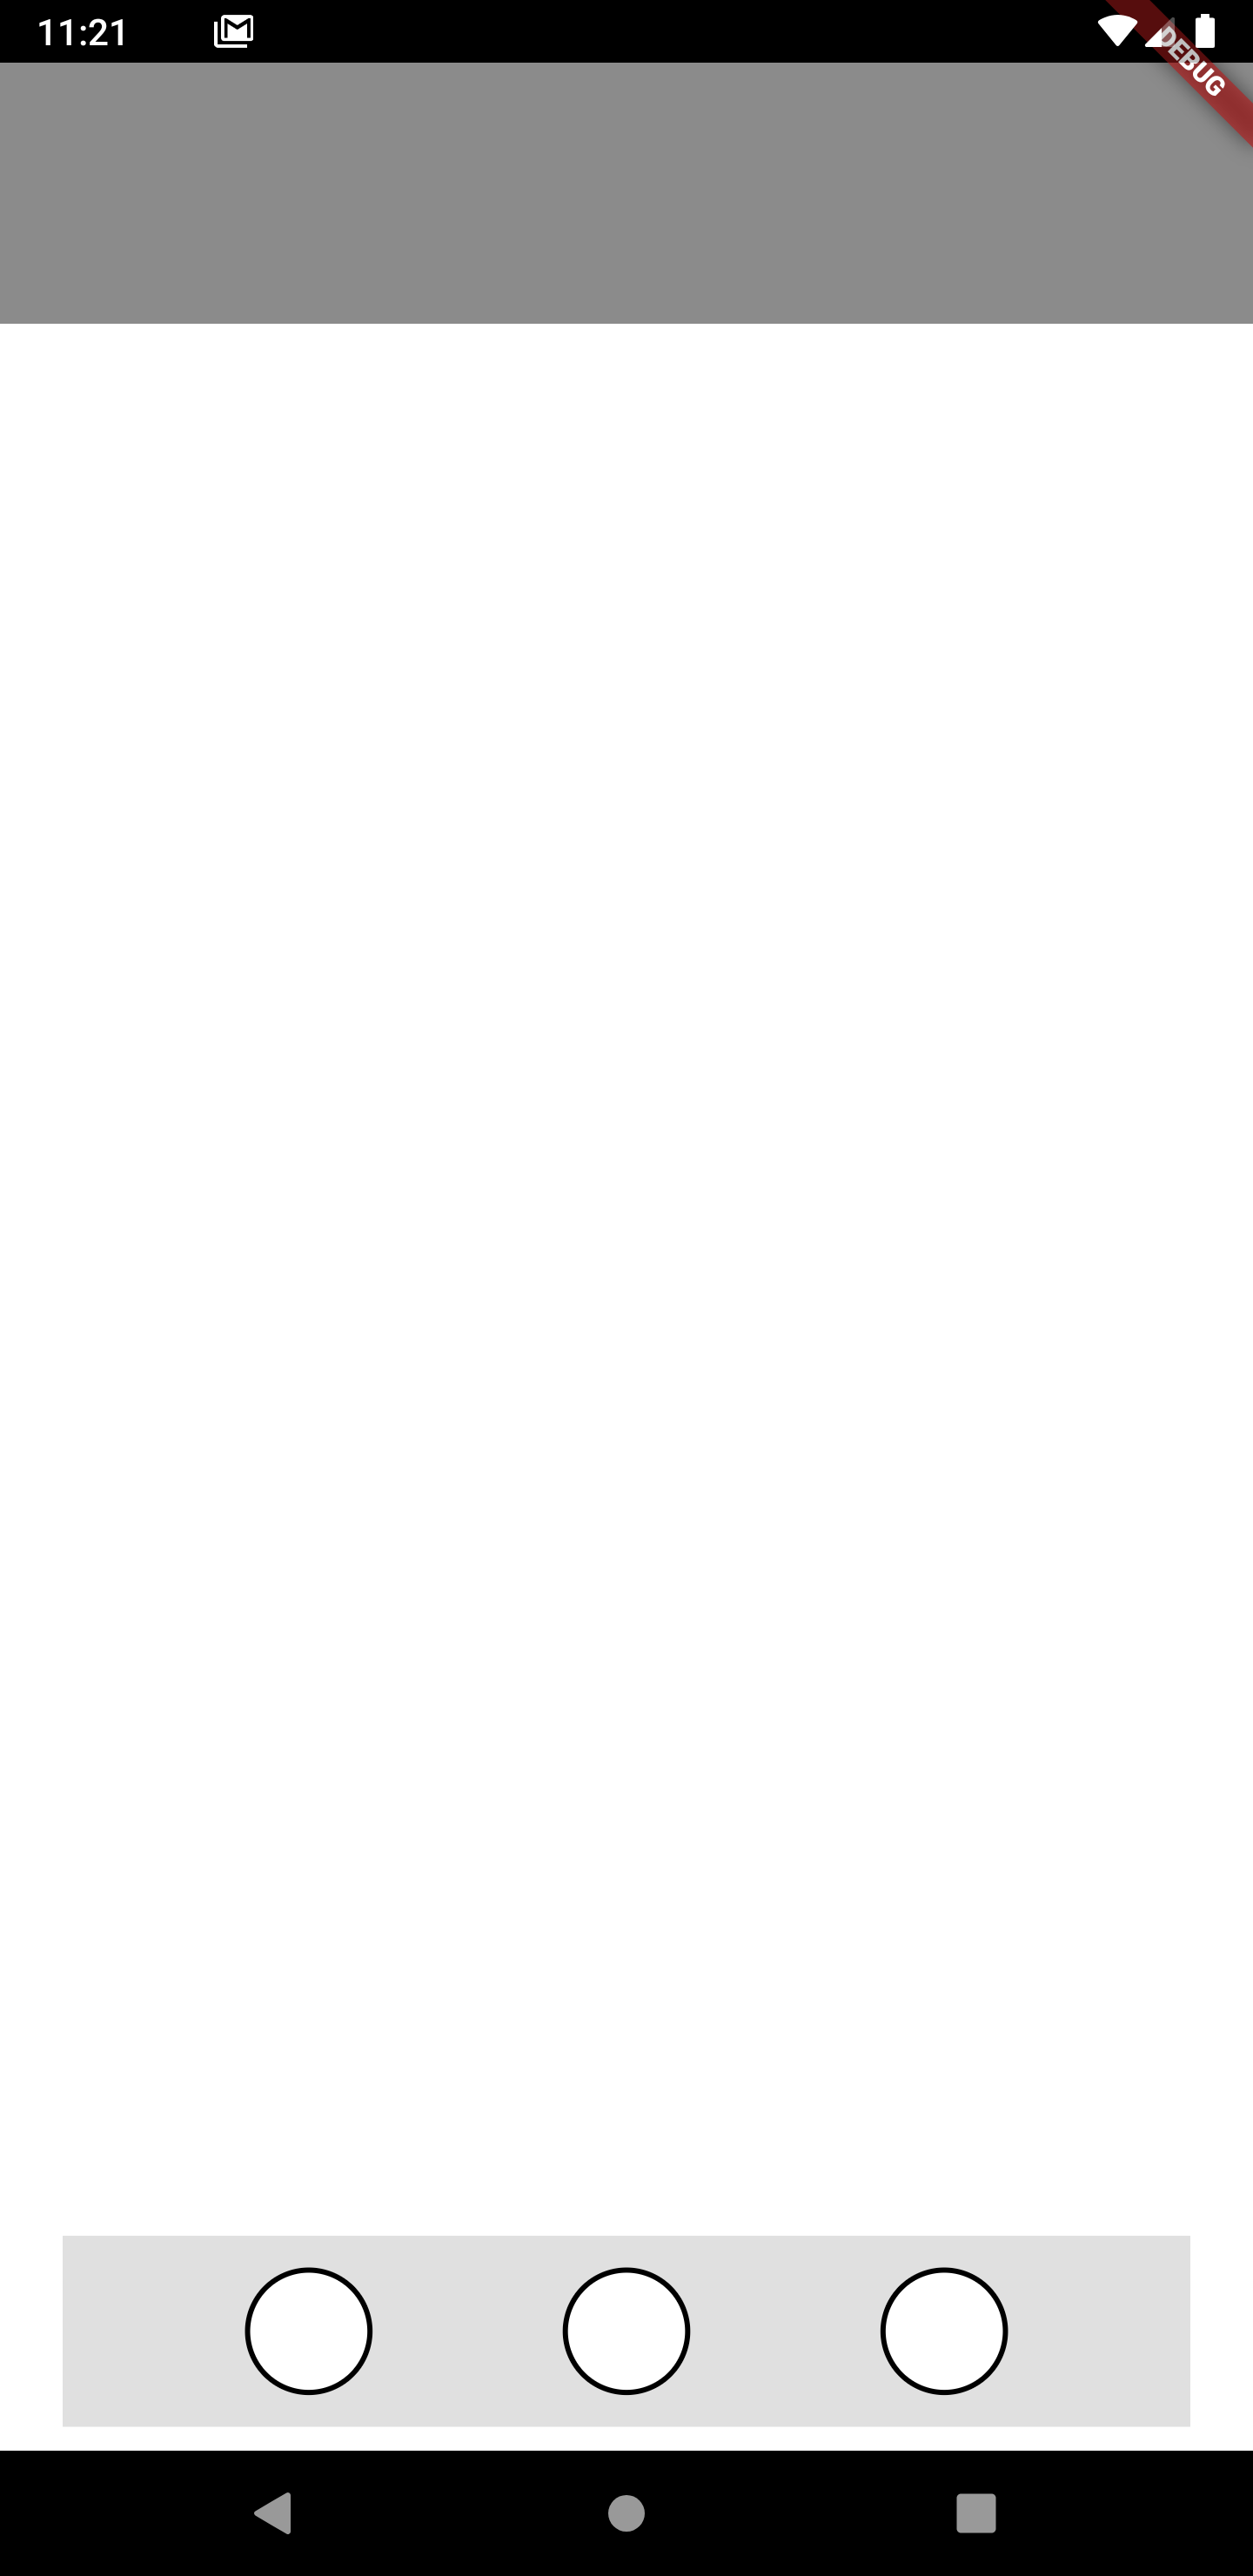
\includegraphics[width=5cm]{Images/App/ymove.png}
        \caption{Value e (4,2) = 100}
        \label{fig:ymove}
    \end{subfigure}
    \caption{Moving the space}
    \label{fig:moving}
\end{figure}

\begin{figure}[b]
    \begin{subfigure}{0.4\textwidth}
        \centering
        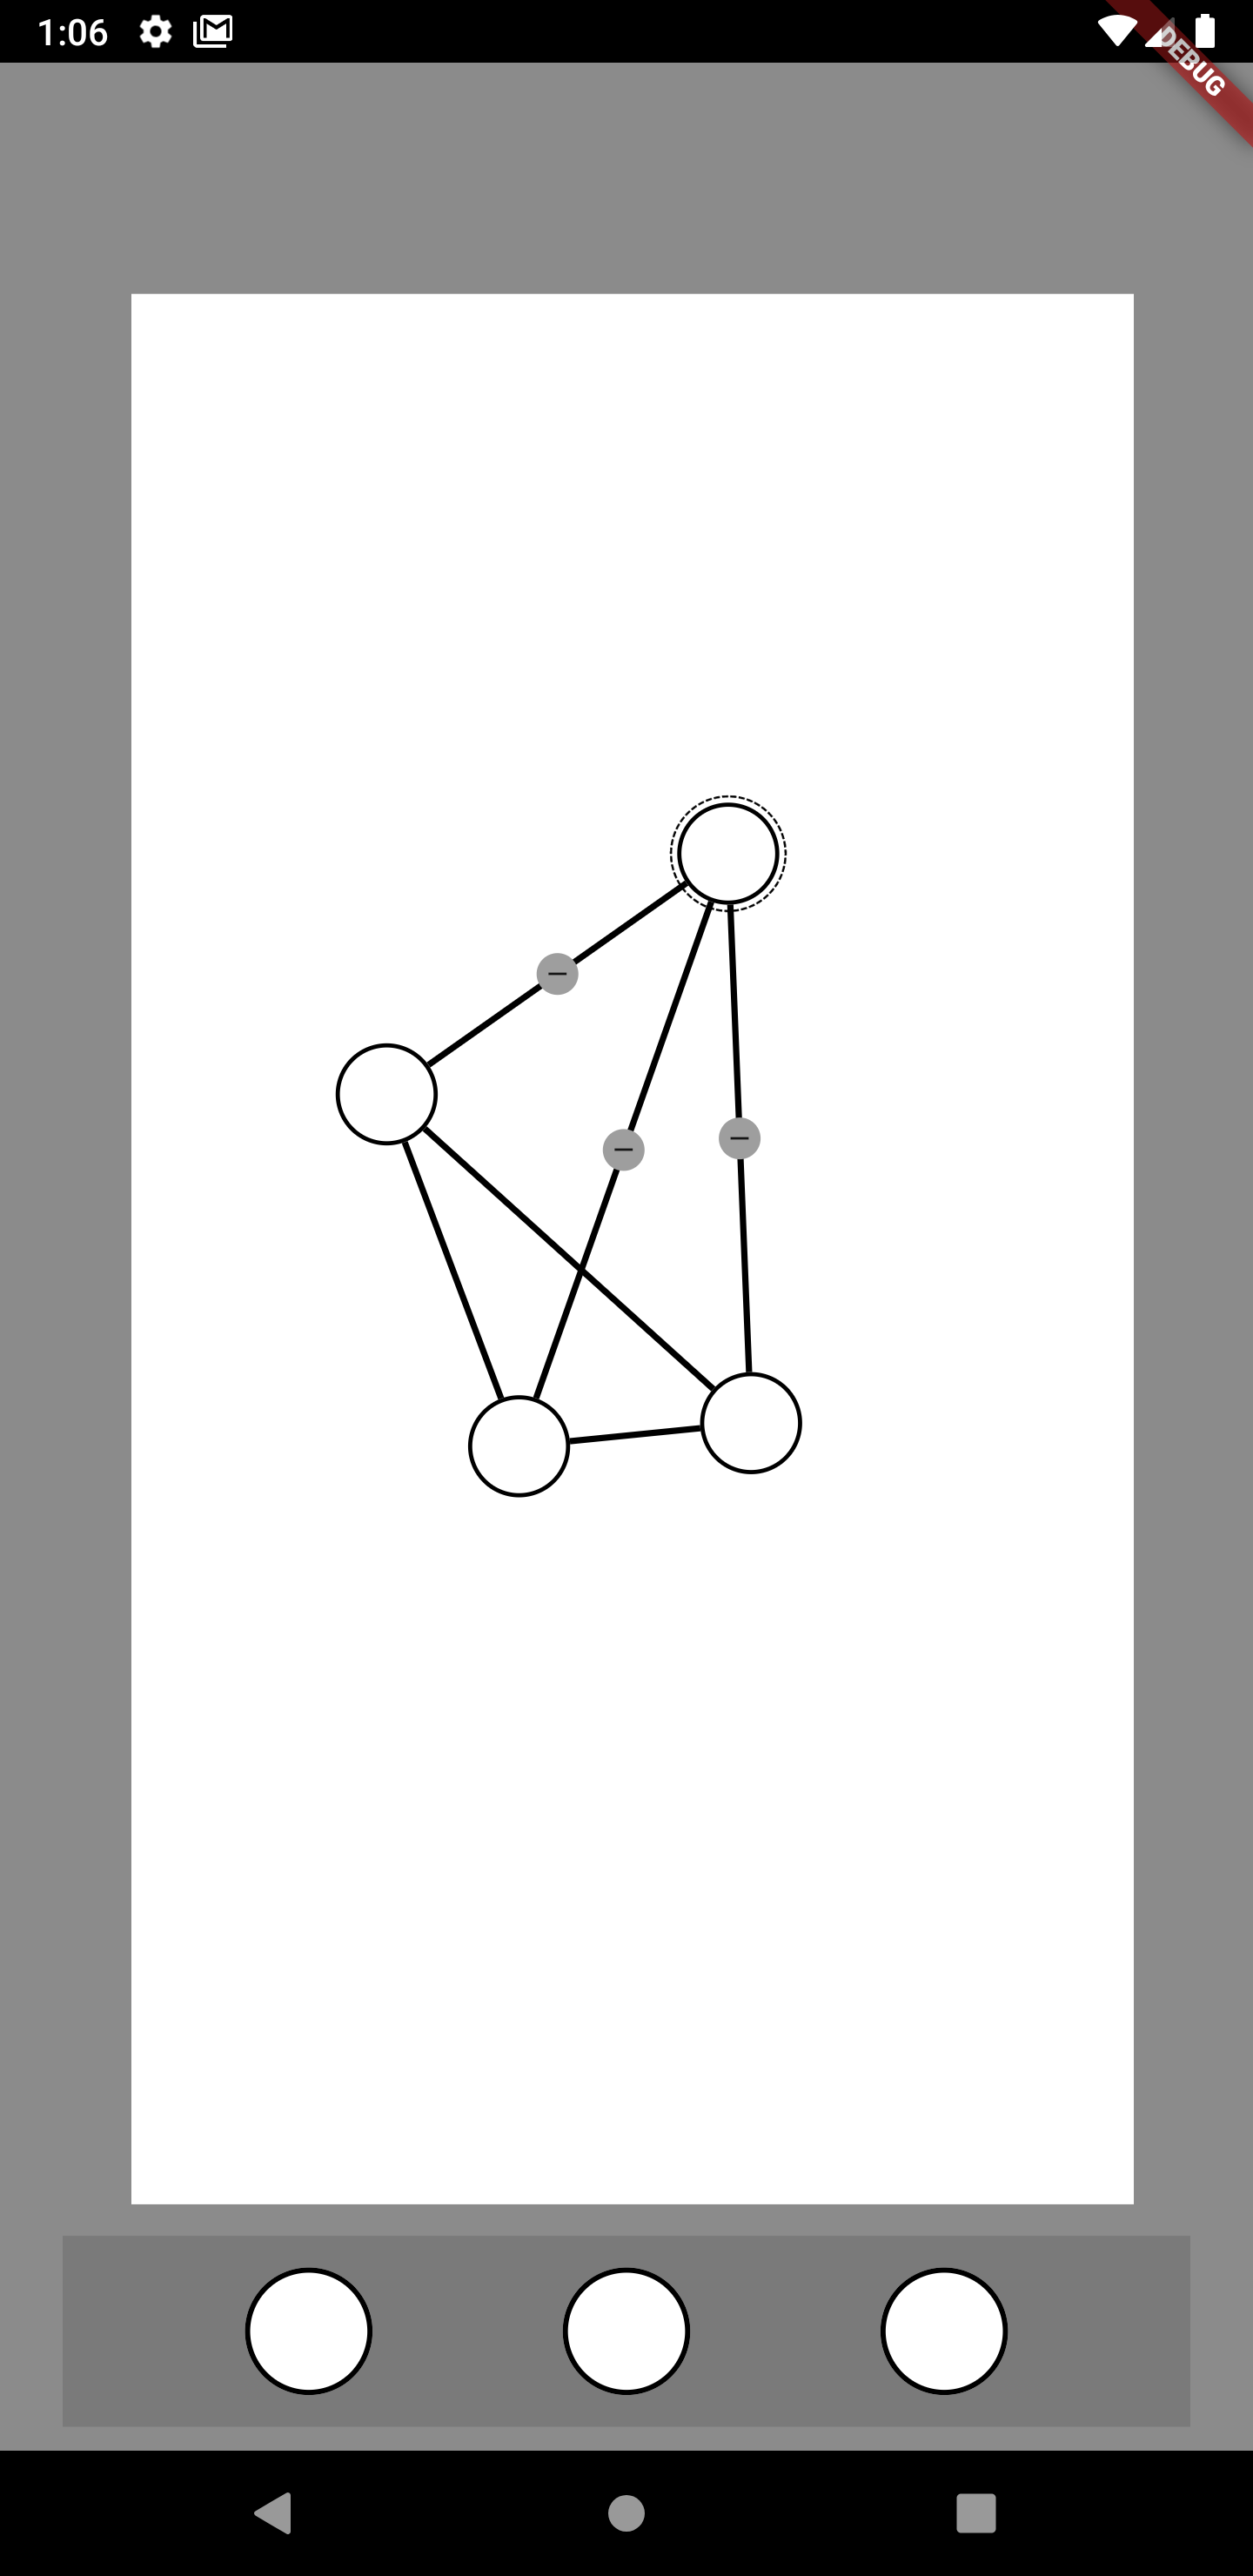
\includegraphics[width=4cm]{Images/App/AppDemo1.png}
        \label{fig:demo1}
    \end{subfigure}
    \hfill
    \begin{subfigure}{0.4\textwidth}
        \centering
        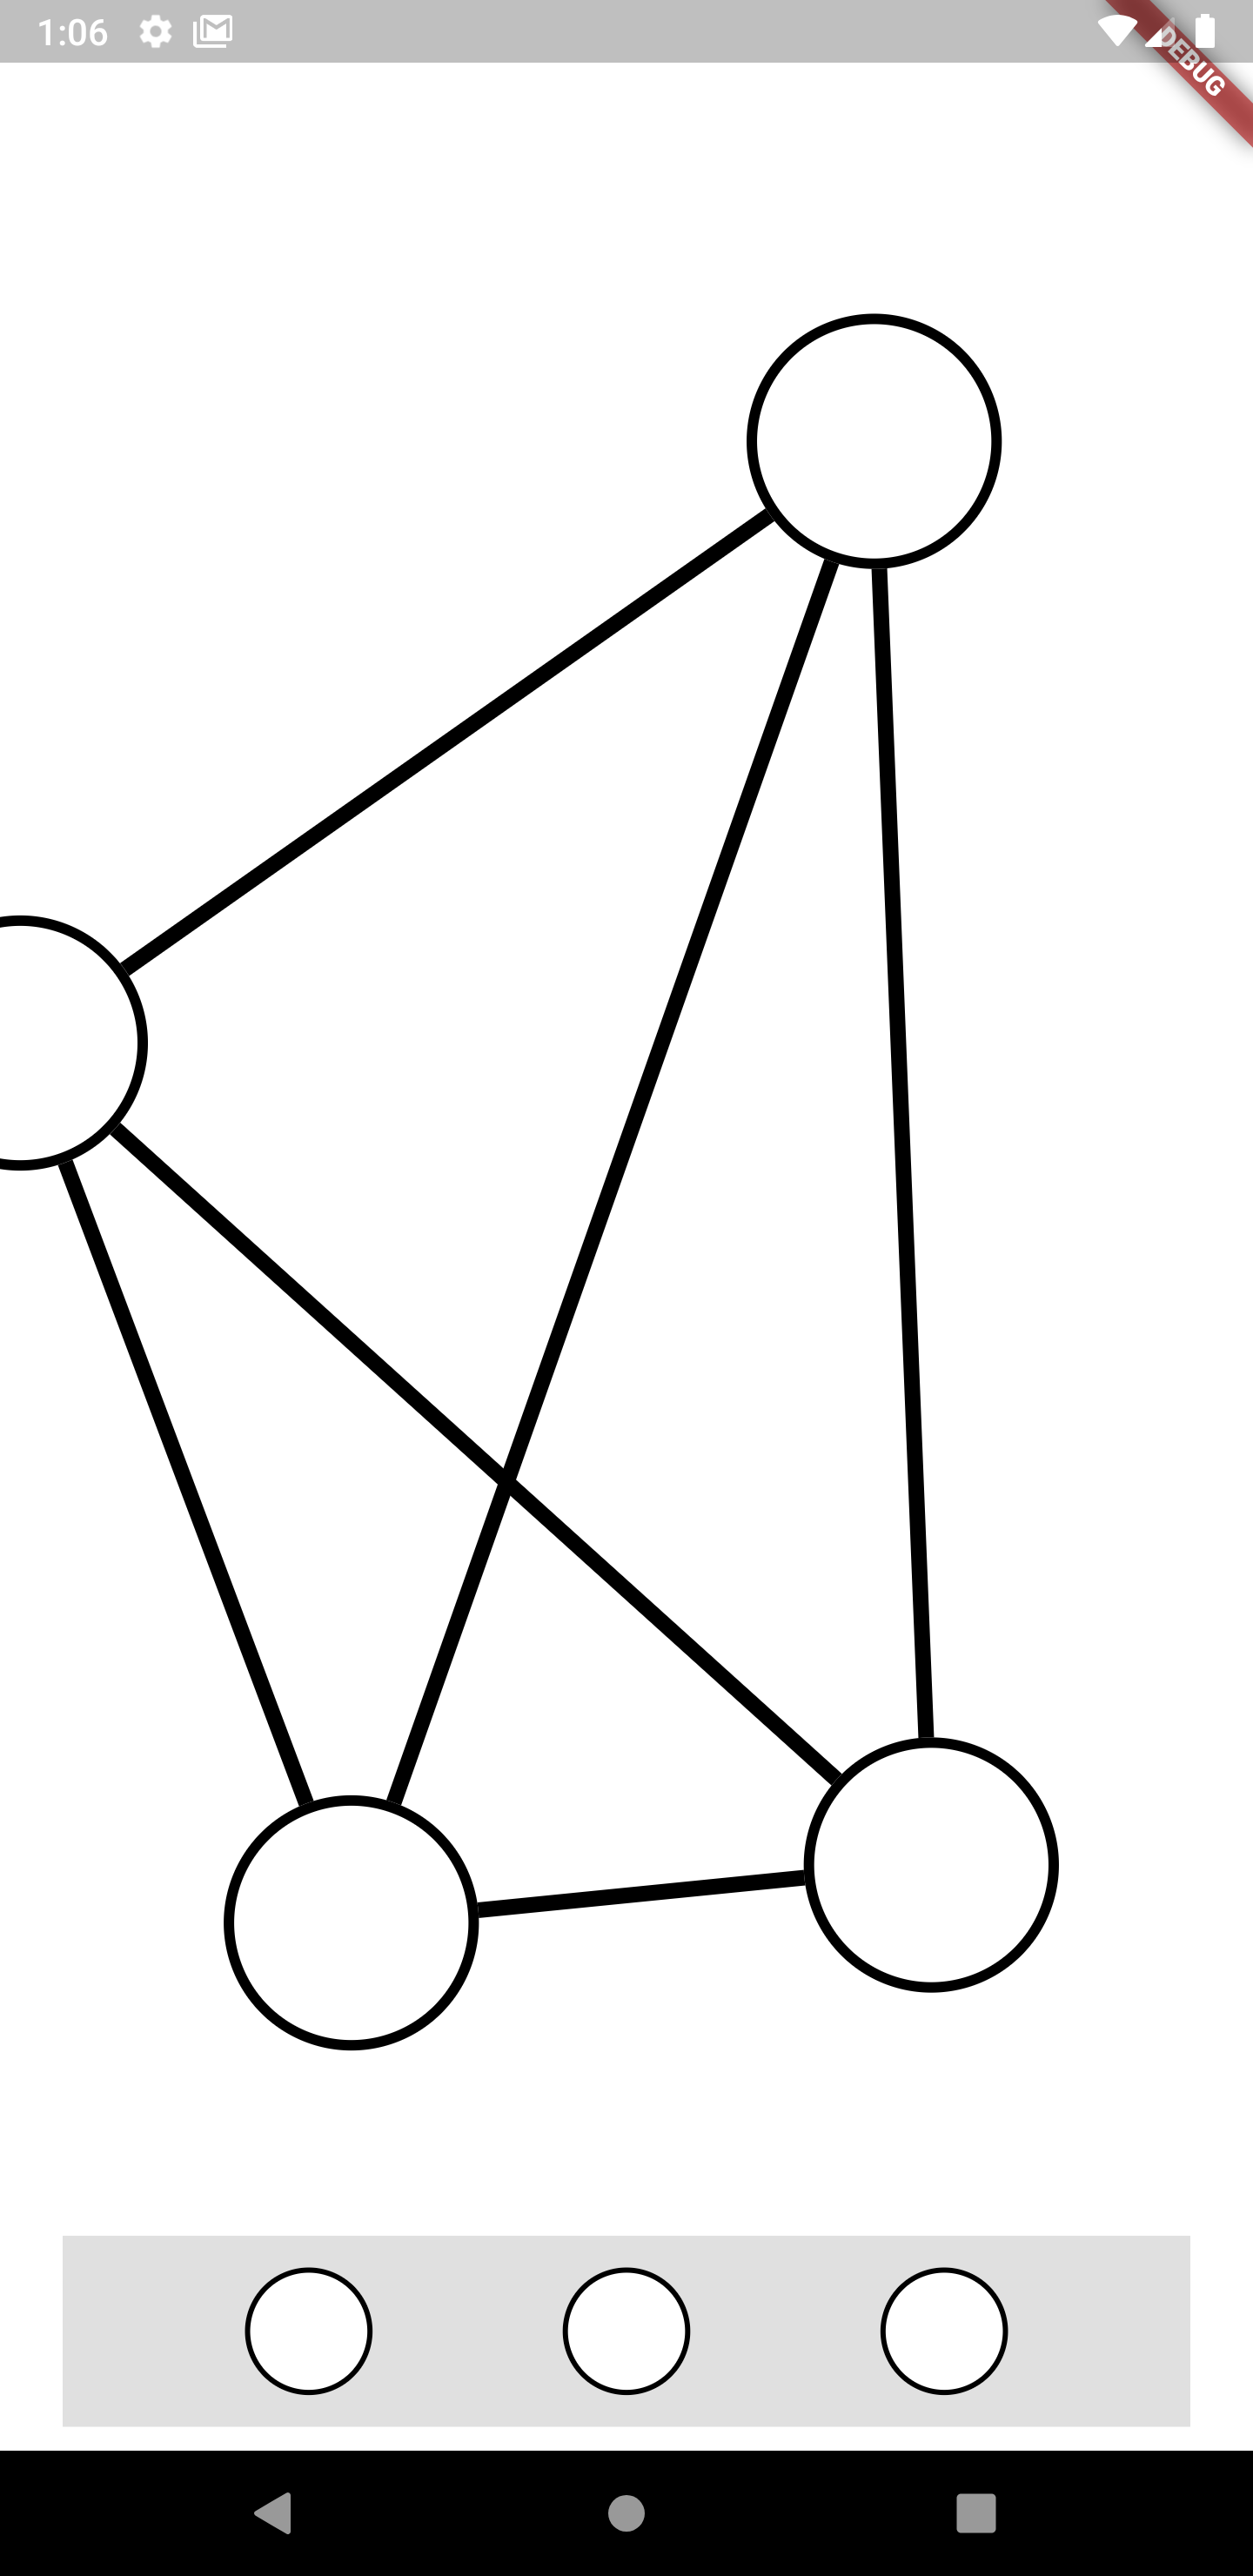
\includegraphics[width=4cm]{Images/App/AppDemo2.png}
        \label{fig:demo2}
    \end{subfigure}
    \caption{Diagram display result}
    \label{fig:result}
\end{figure}


\chapter{Conclusion and Future Work} \label{chap:conclusion}

% \section{conclusion}
% The field diagram detection is an interesting and complex study domain. Although there are many research about on-line diagram, there is still less research about recognizing off-line diagram. With this thesis proposal, we have achieved new background knowledge about the computer vision. We are able to access each procedures in image processing which is also a new field for us. We finds many approaches for handwriting flowchart recognition and we select the suitable approaches using Faster R-CNN, YOLO v4 and RefineDet.\\
% During the research process, our group still had many problems in teamwork, lack of time management skills which affects negatively our result. This problems may become a wall in our work in the future, which we need to overcome and improve our working process.

% \section{Challenges}
% \begin{itemize}
%     \item One of the biggest problem with server-client system is scaling or the amount of customers serving at the same time. Most of our experiment is conducted in the local machine so that there is a need to find a way to provide more stable service in the final product.
%     \item The target is to support a wide range of products so as many devices can install this app as possible. Then it can lead to performance issues and the need to find a balance between stable functioning and feature variety.
%     \item Security is also important since many of these data can be very crucial. All of the information sent or receive by the app and the server need to be secured in order to prevent data leak.
% \end{itemize}

% \section{Future work}
% In the future, we are going to implement the flowchart recognition system and also evaluate the capabilities of the programming languages and the support framework to reduce the constraints of our proposed system while solving all of the listed challenges.

\renewcommand{\bibname}{References}
\bibliography{refs}
\bibliographystyle{unsrt}


\end{document}
